% !TEX root = ../Thesis.tex
\newcommand{\JMu}{\ensuremath{\jpsi\rightarrow\mu\mu}}
\newcommand{\ZMu}{\ensuremath{Z\rightarrow\mu\mu}}
\newcommand{\errt}[2]{\ensuremath{\pm\num{#1}\,\textrm{#2}}}
\newcommand{\fulleff}[4]{\ensuremath{(\num{#1}\errt{#2}{(bkg.)}\,\errt{#3}{(sig.)}\,\errt{#4}{(stat.)})\si{\percent}}}
\newcommand{\Nyield}[2]{\ensuremath{ N^{ \textrm{#1} }_{\textrm{#2}} } }

\chapter[Calibration of the soft muon tagger]{Calibration of the soft muon tagger for 2012 ATLAS data}\label{ch:Calibration}

High-energy physics relies heavily on the use of simulated data to inform the development of analysis techniques. It is paramount that the simulation describe nature as closely as possible. However, the simulation cannot perfectly recreate conditions within the detector and some kinematic variables are not accurately simulated. This includes the quality of matching between ID and MS tracks which are fundamental for the SMT tagger.

Selection and reconstruction techniques are said to be calibrated when the discrepancy between simulation and collision data is quantified. This process has to be repeated on new collision data and/or when simulation is changed in a relevant and significant way.

The difference in efficiency between collision data and simulation of the muon reconstruction procedure and the \xsm\ tagger selection are accounted for by a scale factor (SF),

\begin{equation}
  \textrm{SF} = \frac{\epsilon^{\textrm{Data}}}{\epsilon^{\textrm{MC}}}
\end{equation}
%
which is used to rescale the simulation so that it matches the data more closely. 

One of the advantages of using the \xsm\ tagger over other forms of $b$-tagging is that the presence of a jet is not required to measure the \xsm\ of a muon. This means that the calibration can be performed on isolated muons such as those from \JMu\ or \ZMu\ using the so called tag and probe method. This calibration relies on muons with low \pt\ from \jpsi\ decays. Within ATLAS, the nominal calibration of the reconstruction efficiency is performed on \ZMu\ due to the smaller uncertainty using high \pt\ muons. The SF at low \pt\ are obtained by extrapolating back into the low momentum range.

The tag and probe method is implemented as follows: a STACO combined muon is designated as the \emph{tag}, this muon must pass a stringent set of cuts implying that it is indeed a muon from a \jpsi. The second muon, which is designated as the \emph{probe}, is simply an ID track. To ensure that the probe is the second muon from the \jpsi\ decay, the invariant mass of the combined tag and probe system is required to be in a window centred around the \jpsi\ mass. The complete selection used in the calibration is detailed in Section~\ref{sec:CalibrationSelection}. These probes are used to measure the reconstruction efficiency and the \xsm\ tagger efficiency by using a fit to their invariant mass distribution as described in Section~\ref{sec:CalibrationFitting}. This procedure is performed in various bins of kinematic variables such as transverse momentum and angular position. The binning is described in more detail in Section~\ref{sec:CalibrationBinning}. The results of this analysis are then presented in Section~\ref{sec:CalibrationEfficiencies}.

The procedure used here is based on a previous calibration of the \xsm\ tagger performed on 2011 ATLAS collision data detailed in~\cite{Calibration:MattThesis}. It differs from the 2011 calibration in several ways which will be highlighted and explained.

\subsection*{Software, collision data and simulated samples}

The dataset used is made of those luminosity blocks selected by the recommended standard \emph{good runs list} (GRL) which corresponds to all $pp$ collision periods in 2012. The GRL selects only those luminosity blocks where detector conditions are appropriate for physics data-taking. This requires that all relevant detector components are operational, and that stable beam conditions have been achieved. In total this represents an integrated luminosity of \SI{20.1}{\per\femto\barn}. 

The efficiency scale factor is measured against a sample containing almost 10 million \JMu\ events. At event generation, filters are applied so the sample only contains events where both truth muons have a momentum of at least \SI{4}{\GeV} and they must lie within the pseudorapidity range $|\eta|<2.5$. This selection matches the object selection used by most analyses. 

\section{Tag and probe selection}\label{sec:CalibrationSelection}

The tag and probe procedure is as follows: first, require the presence of a STACO CB muon which passes a very stringent selection. This strongly implies that this is a real muon and thus is labelled as the tag. A very loose selection is then applied to all ID tracks to construct a pool of candidate probes. Pairs of tag and probes are formed by requiring that the combined invariant mass lie within a \jpsi\ mass window and the pair pass additional pairing cuts. This then implies that the probe is likely the other muon from the \jpsi\ decay and as such is a suitable test-bed to measure the performance of the muon reconstruction algorithm. All selection criteria are detailed and explained in Section~\ref{sec:CalibrationSelectionCuts}.

Probes which are reconstructed into STACO CB muons are labelled as muon probes. The reconstruction performance is quantified by the portion of probes, which are likely to be real muons, that are reconstructed into muons. The performance of the \xsm\ tagger is estimated in a similar way, by measuring the proportion of muon probes which are selected by the \xsm\ algorithm.

\subsection{Trigger requirements}\label{sec:CalibrationTriggerRequirement}

In order for an event to be included in the analysis it must have fired at least one of the trigger chains listed in Appendix~\ref{app:CalibrationTrigger}. Only the primary trigger, EF\_mu6\_Trk\_Jpsi\_loose which contributes the majority of events, is described here.

As stated in the trigger name, this is an EF trigger which requires the presence of a muon with a momentum of at least \SI{6}{GeV} and an ID track with a combined invariant mass in the range $\SI{2.6}{GeV}<m_{\textrm{inv}}<\SI{3.6}{GeV}$. This mass window is loose enough to   contain the entirety of the \jpsi\ peak and side-bands that allow for background removal. Double muon triggers are not used to avoid introducing a bias by requiring the presence of two good muons. 

While all triggers are operational in all periods, most are heavily prescaled by a factor which is period dependent. This does not have a first-order effect on the efficiency as only ratios of event yields are compared between collision data and simulation. However, the effective integrated luminosity is reduced to approximately \SI{200}{\per\nano\barn} as a result of the prescale. A short study was carried out to examine the effects of multiple prescaled triggers on the scale factors. The measurement was carried out using only the primary trigger and the results were compared to the nominal calibration which included all the triggers, no significant discrepancy between the two was observed.

\subsection{Selection cuts}\label{sec:CalibrationSelectionCuts}

The selection criteria for tags, probes, muon probes and SMT muons are listed and detailed below. All cuts are applied on the kinematic properties as measured in the ID due to its better resolution. Also note that all objects must pass a set of track quality criteria as recommended by the ATLAS \emph{muon combined performance} (MCP) group. These cuts require a certain number of detector elements be active to ensure good quality track reconstruction. The selection criteria are listed in Appendix~\ref{app:CalibrationMCPCuts}.

The tag selection is summarized in Table~\ref{tab:CalibrationTagSelection}. The tag is a STACO combined muon with a pseudorapdity and transverse momentum that allow for reliable reconstruction. The requirements on the impact parameter variables are in place to remove spurious muons from pile-up events and the decay-in-flight of long-lived hadrons. Finally, the tag muon is required to have fired at least one of the triggers under which the event was recorded. This is done by matching the reconstructed trigger object to the tag muon via a $\Delta R$ cut of less than \num{0.01}.

\begin{table}
  \centering
    \begin{tabular}{@{}ll@{}}
    \toprule
    \multicolumn{2}{c}{Tag selection} \\
    \midrule
    \multirow{3}{*}{Reconstruction cuts} & STACO combined muon \\
                                      & $|\eta|<2.5$ \\
                                      & $\pt>\SI{4}{\GeV}$ \\
    \multirow{4}{*}{Pileup reduction} & $|d_{0}|<\SI{0.3}{\mm}$ \\ 
                                      & $|z_{0}|<\SI{1.5}{\mm}$ \\
                                      & $|d_{0}/\sigma_{d_{0}}|<3$ \\
                                      & $|z_{0}/\sigma_{z_{0}}|<3$ \\
    \bottomrule  
    \end{tabular}
    \caption{Tag selection criteria.}\label{tab:CalibrationTagSelection}
\end{table}

The probe selection is a subset of the tag selection and only requires an ID track with $|\eta|<2.5$ and $\pt>\SI{4}{\GeV}$. 

The pairing selection, summarized in Table~\ref{tab:CalibrationPairingSelection}, is designed to construct pairs tag and probe candidates which likely come from the same \jpsi\ decay. The main component of the selection is the invariant mass window cut. The tag and the probe are required to be well separated in $\eta$-$\phi$ space to prevent the objects from entering each others isolation cones.

\begin{table}[htbp]
  \centering
    \begin{tabular}{@{}ll@{}}
      \toprule
      \multicolumn{2}{c}{Pairing criteria} \\
      \midrule
      Opposite charge   & $q_{\textrm{tag}} \neq q_{\textrm{probe}}$ \\
      Mass window       & $|m_{\jpsi}-m_{\textrm{tag, probe}}|\leq\SI{2}{\GeV}$ \\
      Overlap reduction & $0.2<\Delta R^{\textrm{tag}}_{\textrm{probe}}<3.5$ \\
      Pileup reduction  & $\Delta z_{0}<\SI{0.2}{\mm}$ \\
      \bottomrule
    \end{tabular}
    \caption{Pairing criteria.}\label{tab:CalibrationPairingSelection}
\end{table}

In the 2011 calibration analysis, the track of the tag and the probe were refitted to a common vertex and the quality of the refit, expressed by a $\chi^2$, was part of the pairing criteria. This cut is meant to reduce the effects of pile-up on the measurement by ensuring both objects have a common origin. Due to operational reasons it is not possible to perform the refitting in this case. Instead, a cut on $\Delta z_{0}=|z_{0,\textrm{ tag}}-z_{0,\textrm{ probe}}|$ is applied. If several pairings are made for a single tag, the pair with the smallest $\Delta z_{0}$ is used.

The STACO CB reconstruction efficiency is not measured by applying the algorithm on the probe collection but rather a probe is said to be a muon probe if it matches a combined muon from the STACO collection. This is done by requiring the \DeltaR\ between the probe and the STACO CB muon be less than \num{0.01}. Probes which are matched become the numerator of the reconstruction efficiency and the denominator is defined as the number of probes:

\begin{equation}
  \epsilon_{\textrm{reco}} = \frac{N_{\textrm{muon probe}}}{N_{\textrm{probe}}}
\end{equation}

A muon probe is said to be an SMT muon if it passes the selection listed in Table~\ref{tab:CalibrationSMTSelection} that matches the cuts defined in Section~\ref{sec:DetectorSLT}. The \xsd\ distribution of muon probes is shown in Figure~\ref{fig:CalibrationMatchChi2Dist}.

\begin{table}[htbp]
  \centering
    \begin{tabular}{@{}ll@{}}
      \toprule
      \multicolumn{2}{c}{SMT selection} \\
      \midrule
      \multirow{2}{*}{Pileup reduction} & $|d_{0}|<\SI{3}{\mm}$ \\
                            & $|z_{0}\sin(\theta)|<\SI{3}{\mm}$ \\
      Match quality         & $\xsm/\ndof<3.2$ \\
      \bottomrule
    \end{tabular}
    \caption{SMT criteria.}\label{tab:CalibrationSMTSelection}
\end{table}

\begin{figure}[htbp]
  \centering
    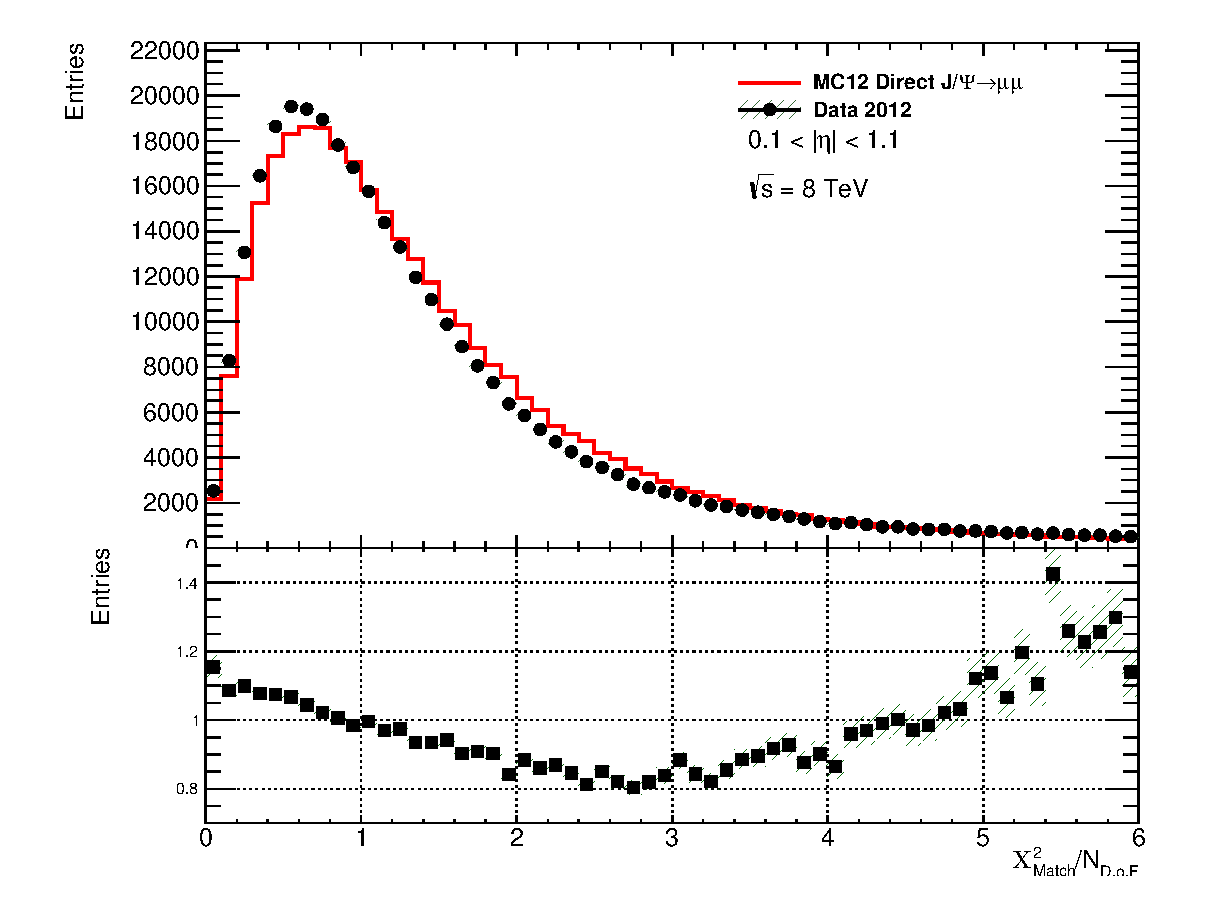
\includegraphics[width=0.75\textwidth]{PartCalibration2012/Plots/Kinematics/h_muonprobe_matchchi2_ndof_Nominal.eps}
    \caption[The distribution of \xsd\ for all muon probes for ATLAS collision data and prompt simulated \jpsi.]{The distribution of \xsd\ for all muon probes for ATLAS collision data (solid dots) and simulated prompt \jpsi\ (dotted line). Note that the collision data distribution includes sources of background.}\label{fig:CalibrationMatchChi2Dist}
\end{figure}

The denominator of the SMT efficiency is the number of muon probes and the numerator is the number of muon probes which pass the SMT selection:

\begin{equation}
  \epsilon_{\textrm{SMT}} = \frac{N_{\textrm{SMT}}}{N_{\textrm{muon probe}}}
\end{equation}

\section{Invariant mass fitting}\label{sec:CalibrationFitting}

The pairing criteria are very effective at selecting \jpsi\ events, however non-\jpsi\ background events also pass the selection. These include combinatorial background where the wrong tag and probe pair is constructed, and Drell-Yan which appears as a continuum below the \jpsi\ peak.

The number of probes is extracted from a fit to the invariant mass of the dimuon system. The invariant mass is fitted with the sum of a quadratic polynomial, for the background; and a Gaussian function, for the signal. The yield is obtained by subtracting the integral of the background function from the binned data, this is used instead of relying on an accurate fit to the signal peak.

The integration is performed in a window with a width three times larger than the width of the fitted Gaussian, denoted as $3\sigma$ in Figure~\ref{fig:CalibrationFittingExample}. The composite fit line, the background-only distribution and the implied signal Gaussian peak are also shown.

\begin{figure}[htbp]
  \centering
    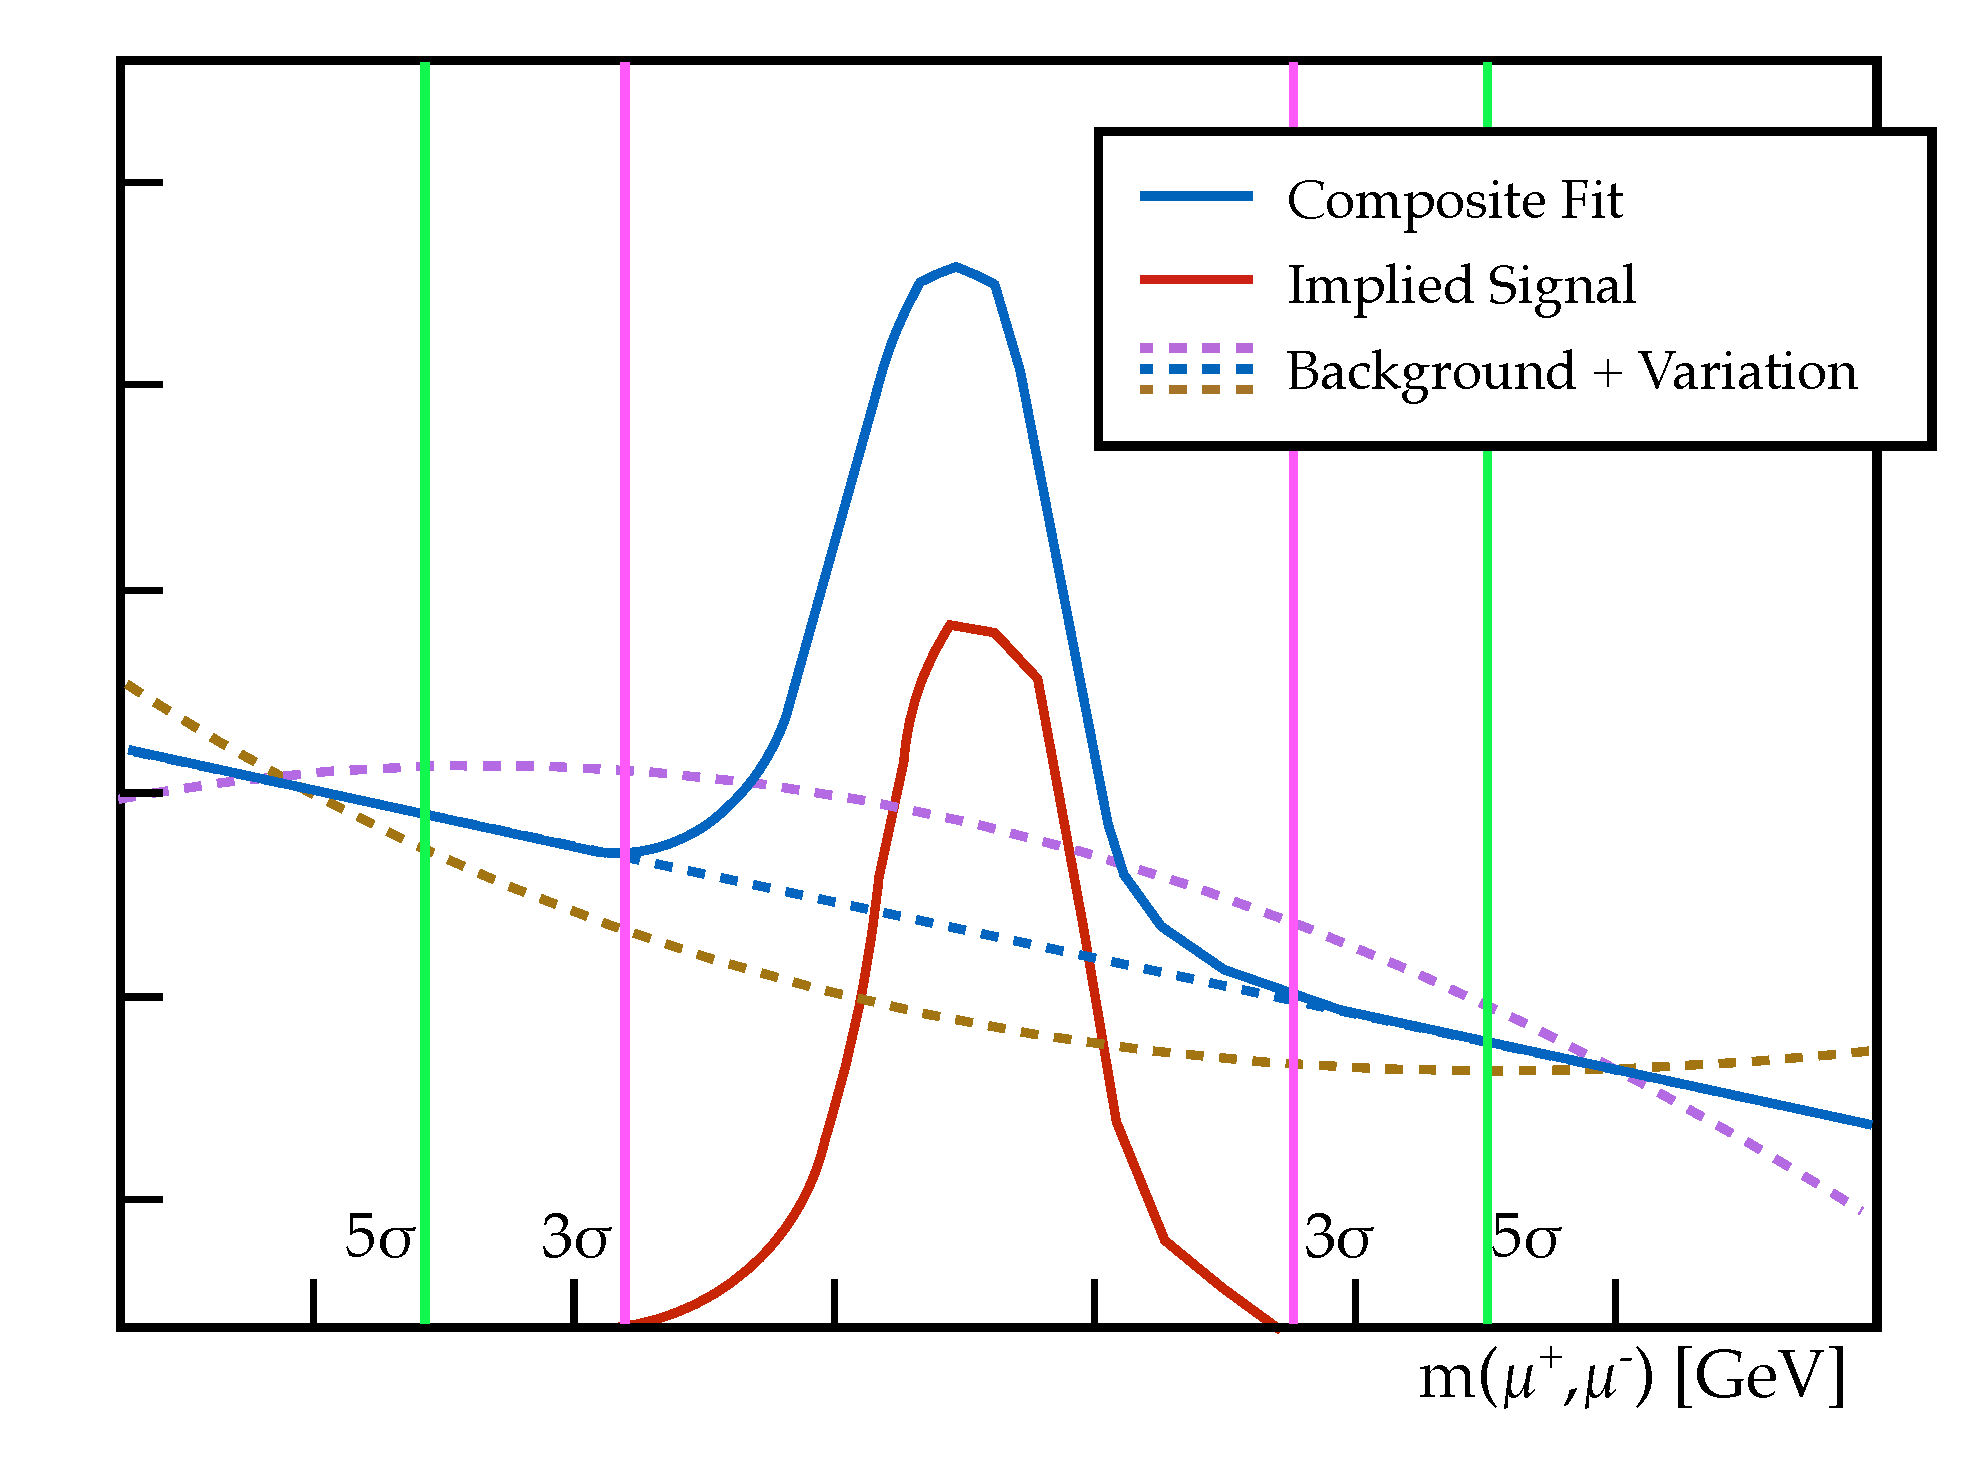
\includegraphics[width=0.75\textwidth]{PartCalibration2012/Plots/FittingExample.pdf}
    \caption[Drawing of the components of the fitting procedure.]{Drawing of the components of the fitting procedure. The composite fit is shown along with the corresponding implied signal and background. The two variations of the background shape are also shown, these are exaggerated for illustration purposes.}\label{fig:CalibrationFittingExample}
\end{figure}

The \jpsi\ peak does not follow a Gaussian shape exactly, but rather the best fit is obtained by the so-called Crystal Ball function shown in Figure~\ref{fig:CalibrationCBDist}. This is a convolution of a Gaussian function with a power tail at low invariant mass to account for the energy loss due to photon emission.

\begin{figure}[htbp]
  \centering
  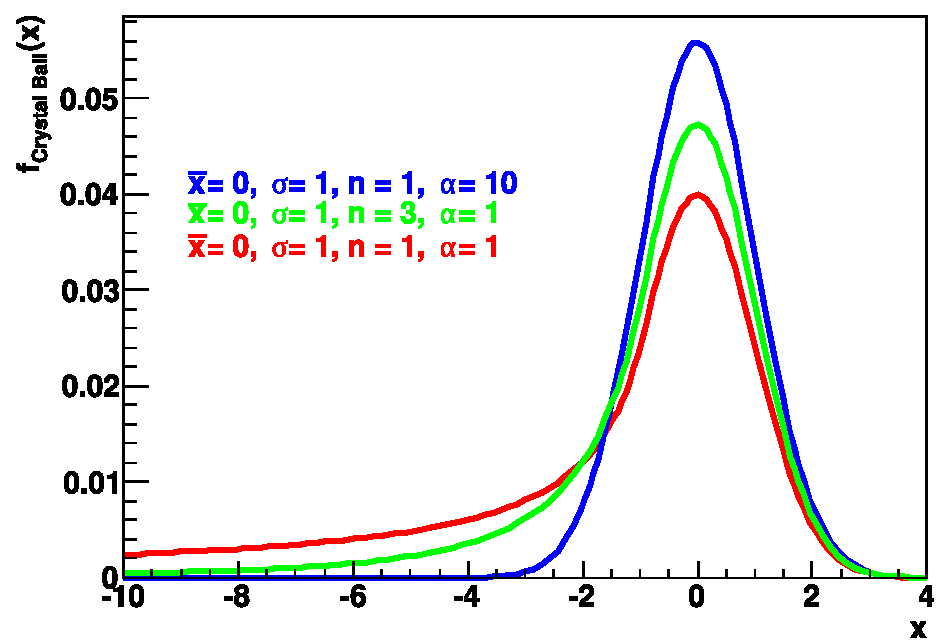
\includegraphics[width=0.75\textwidth]{PartCalibration2012/Plots/CrystalBallFunction.pdf}
  \caption[Diagram of crystal ball distributions with varying tail sizes.]{Diagram of crystal ball distributions with varying tail sizes~\cite{Calibration:CBFunction}. The parameters $\bar{x}$ and $\sigma$ are the mean and width of the Gaussian, while $\alpha$ and $n$ respectively determine the start and shape of the power-tail.}\label{fig:CalibrationCBDist}
\end{figure}

Different combinations of signal and background functions were tested to determine the most stable combination. For the signal, the sum of two Gaussian functions was tested, while for the background a linear function, an exponential function, and the sum of two exponential functions were tried. It was found that none of these yielded good stable fits in the entire pseudorapidity range. For example, the linear function resulted in a mismodelling of the background at the probe level which led to negative efficiencies or extremely large uncertainties. 

From an operational perspective, using a Gaussian function allowed for good stable fits over the hundreds of bins used, and simplified the fitting procedure as a whole. Any mismodelling of the background because of the choice of a Gaussian in lieu of the Crystal Ball fit, is taken into account by the background uncertainty described in the next section.

Several different sets of initial fit conditions were tested and those which yielded the best and most stable fits across the entire $\eta$ and \pt\ range were used. 

The width at the probe level is obtained from the fit and is then used in the fits to the muon probe and SMT distributions. The mean is obtained independently from the fit to each individual distributions. The mean is expected to lie very close to the true \jpsi\ mass, however this is not forced in the fitting procedure. Instead the fit is allowed to set the mean in a window with a width of approximately \SI{1.2}{\GeV}. 

\subsection{Uncertainty measurement}\label{sec:CalibrationUncertainty}

The uncertainty on the efficiency is made up of three components: the statistical uncertainty on the efficiency is estimated as a binomial error,
%
\begin{equation}
  \sigma_{\textrm{stat.}} = \sqrt{\frac{\epsilon(1-\epsilon)}{N}}
\end{equation}
%
where $\epsilon$ is the measured efficiency and $N$ is, in this case the denominator of the efficiency measured.

The second component of the efficiency uncertainty quantifies the error in the background fit. The uncertainty is determined by constructing two functions that denote the maximum upward and downward fluctuation of the background fit. The efficiency is measured using one of these fluctuations and the result is compared to the nominal efficiency.

After the fit of the composite function is carried out, a downward variation of the background is defined as:
%
\begin{equation}
  f^{\textrm{down}}(x) = a_{\min}x^{2} + b_{\max}x + c_{\min}
\end{equation}
%
where the maximum and minimum the parameters ($X_{\min/\max}$) are obtained by varying the central value by the uncertainty obtained from the fit,
%
$X_{\max/\min}=X_{\textrm{central}}\pm\sigma_{X}$

The upward variation of the background fit is defined as the opposite:
%
\begin{equation}
  f^{\textrm{up}}(x) = a_{\max}x^{2} + b_{\min}x + c_{\max}
\end{equation}

These background variations result in the maximum deviation from the nominal integral (Figure~\ref{fig:CalibrationFittingExample}). The uncertainty on the efficiency is determined by obtaining the maximum efficiency in both directions. If the nominal efficiency is defined as
%
\begin{equation}
  \epsilon_{\textrm{nominal}} = \frac{\Nyield{nominal}{numerator}}{\Nyield{nominal}{denominator}}
\end{equation}
%
then the variations are defined as,
%
\begin{equation}
  \epsilon_{\textrm{up}} = \frac{\Nyield{up}{numerator}}{\Nyield{down}{denominator}}%
  \textrm{,}\qquad%
  \epsilon_{\textrm{down}} = \frac{\Nyield{down}{numerator}}{\Nyield{up}{denominator}}
\end{equation}
%
where \Nyield{up/down}{}\ are the yields obtained from the integration of the upward/downward variations of the background function.

Finally the uncertainty on the background is given by the average of the differences between $\epsilon_{\textrm{up}}$ and $\epsilon_{\textrm{down}}$, and the nominal efficiency:
%
\begin{equation}
  \sigma_{\textrm{bkg}} = \frac{1}{2}(|\epsilon_{\textrm{up}}-\epsilon_{\textrm{nominal}}| + |\epsilon_{\textrm{down}}-\epsilon_{\textrm{nominal}}|)
\end{equation}

The final component of the uncertainty is obtained by varying the integration window. The nominal value is defined as $3\sigma_{\textrm{gaus}}$ away from the centre of the fitted Gaussian. An uncertainty is constructed by measuring the efficiency with a wide integration window corresponding to $5\sigma$. The integration window uncertainty is defined as:
%
\begin{equation}
  \sigma_{\textrm{sig.}} = |\epsilon_{5\sigma}-\epsilon_{3\sigma}|
\end{equation}

The total uncertainty on the efficiency is given by the sum in quadrature of all the uncertainty components. The uncertainty on the efficiency is then carried over to the scale factor determination.
As expected the invariant mass distribution for all probes contains a large amount of background, particularly in data (Figure~\ref{fig:CalibrationFittingResult}). The ``shoulders'' at each side of the \jpsi\ peak are the result of the main \jpsi\ trigger which includes a mass window cut more stringent than that required by the pairing selection. Requiring that the probe match a STACO CB muon greatly reduces the amount of background. Applying the SMT requirements also reduces the background though not as substantially.

\begin{figure}[thbp]
  \centering
    \begin{subfigure}[b]{0.80\textwidth}
    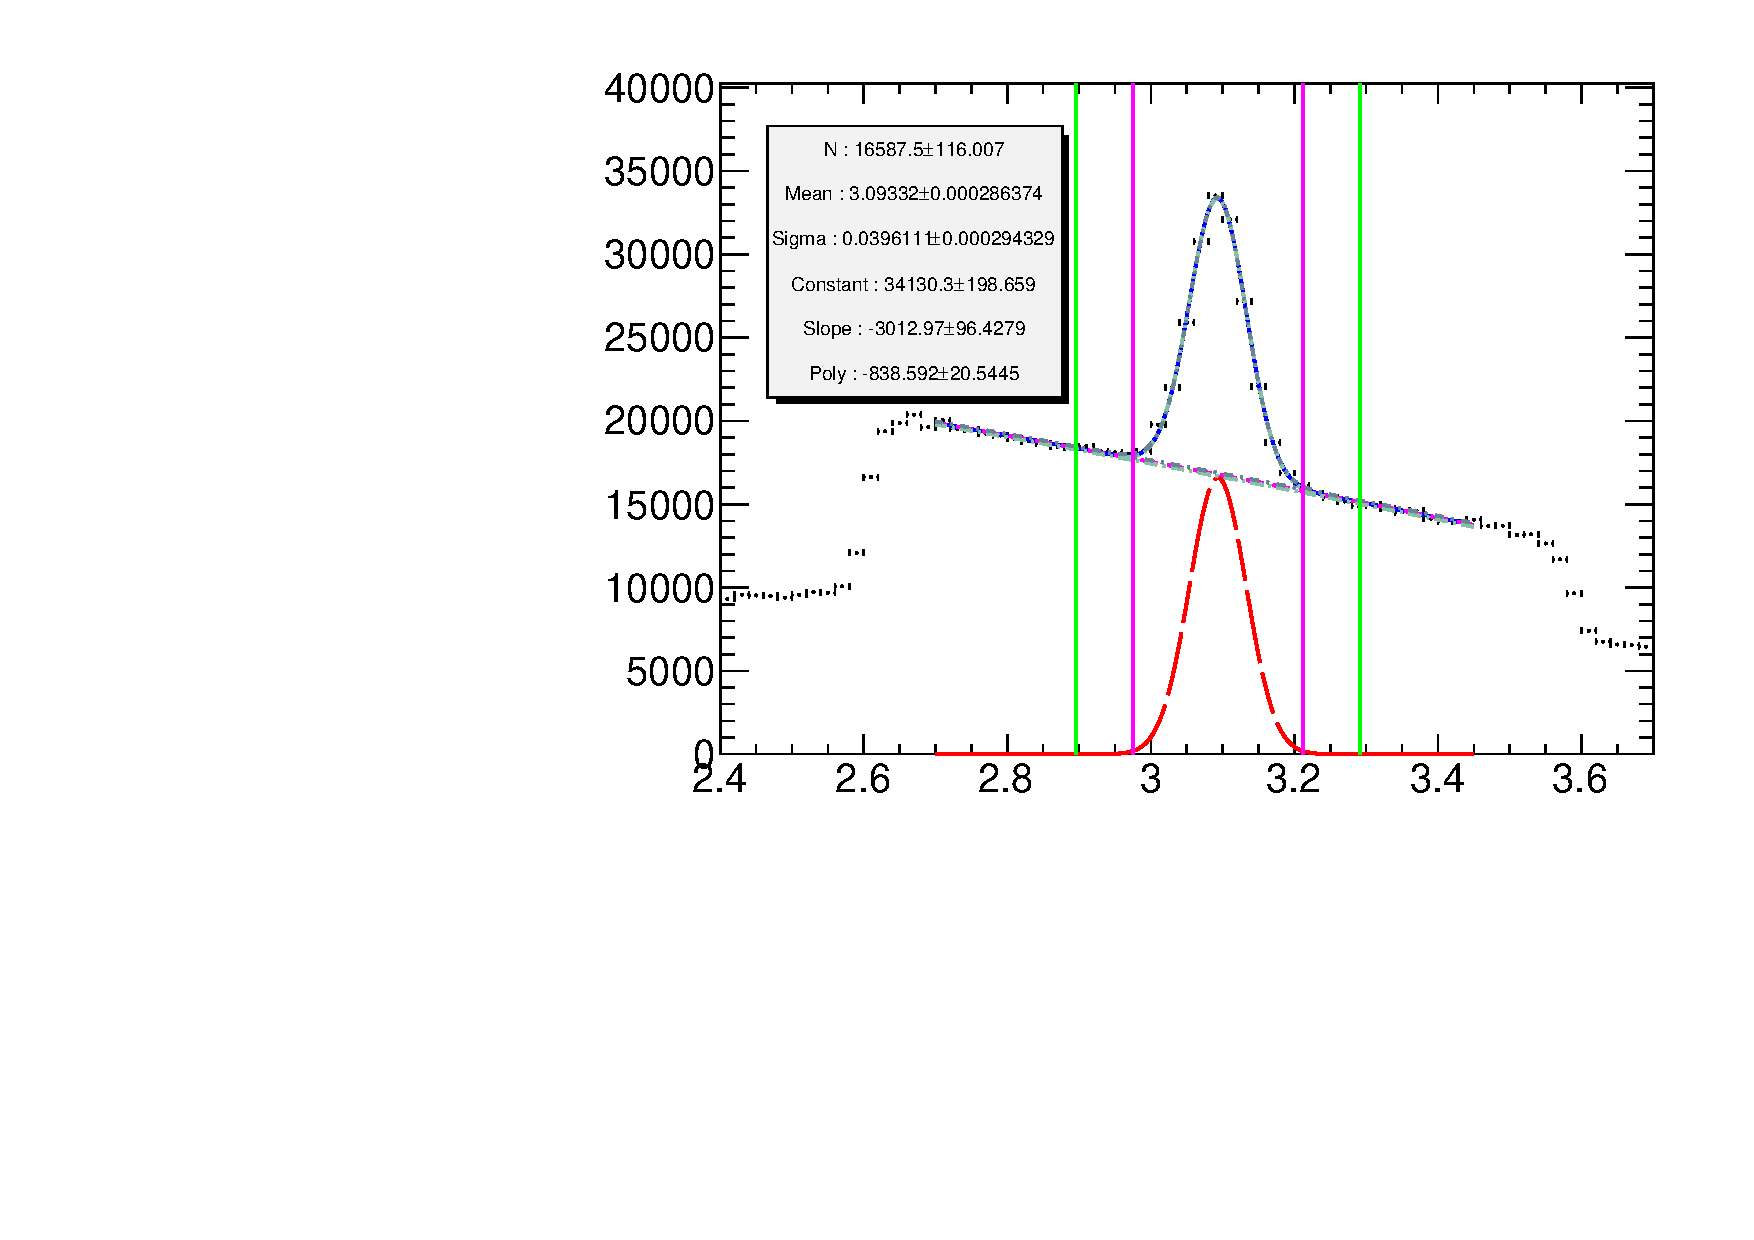
\includegraphics[width=\textwidth]{PartCalibration2012/Plots/Kinematics/Data_InvMass_pt_5_6_barrel_probe.pdf}
      \caption{Probe level}\label{fig:CalibrationInvMassProbe}
    \end{subfigure}

    \begin{subfigure}[b]{0.80\textwidth}
      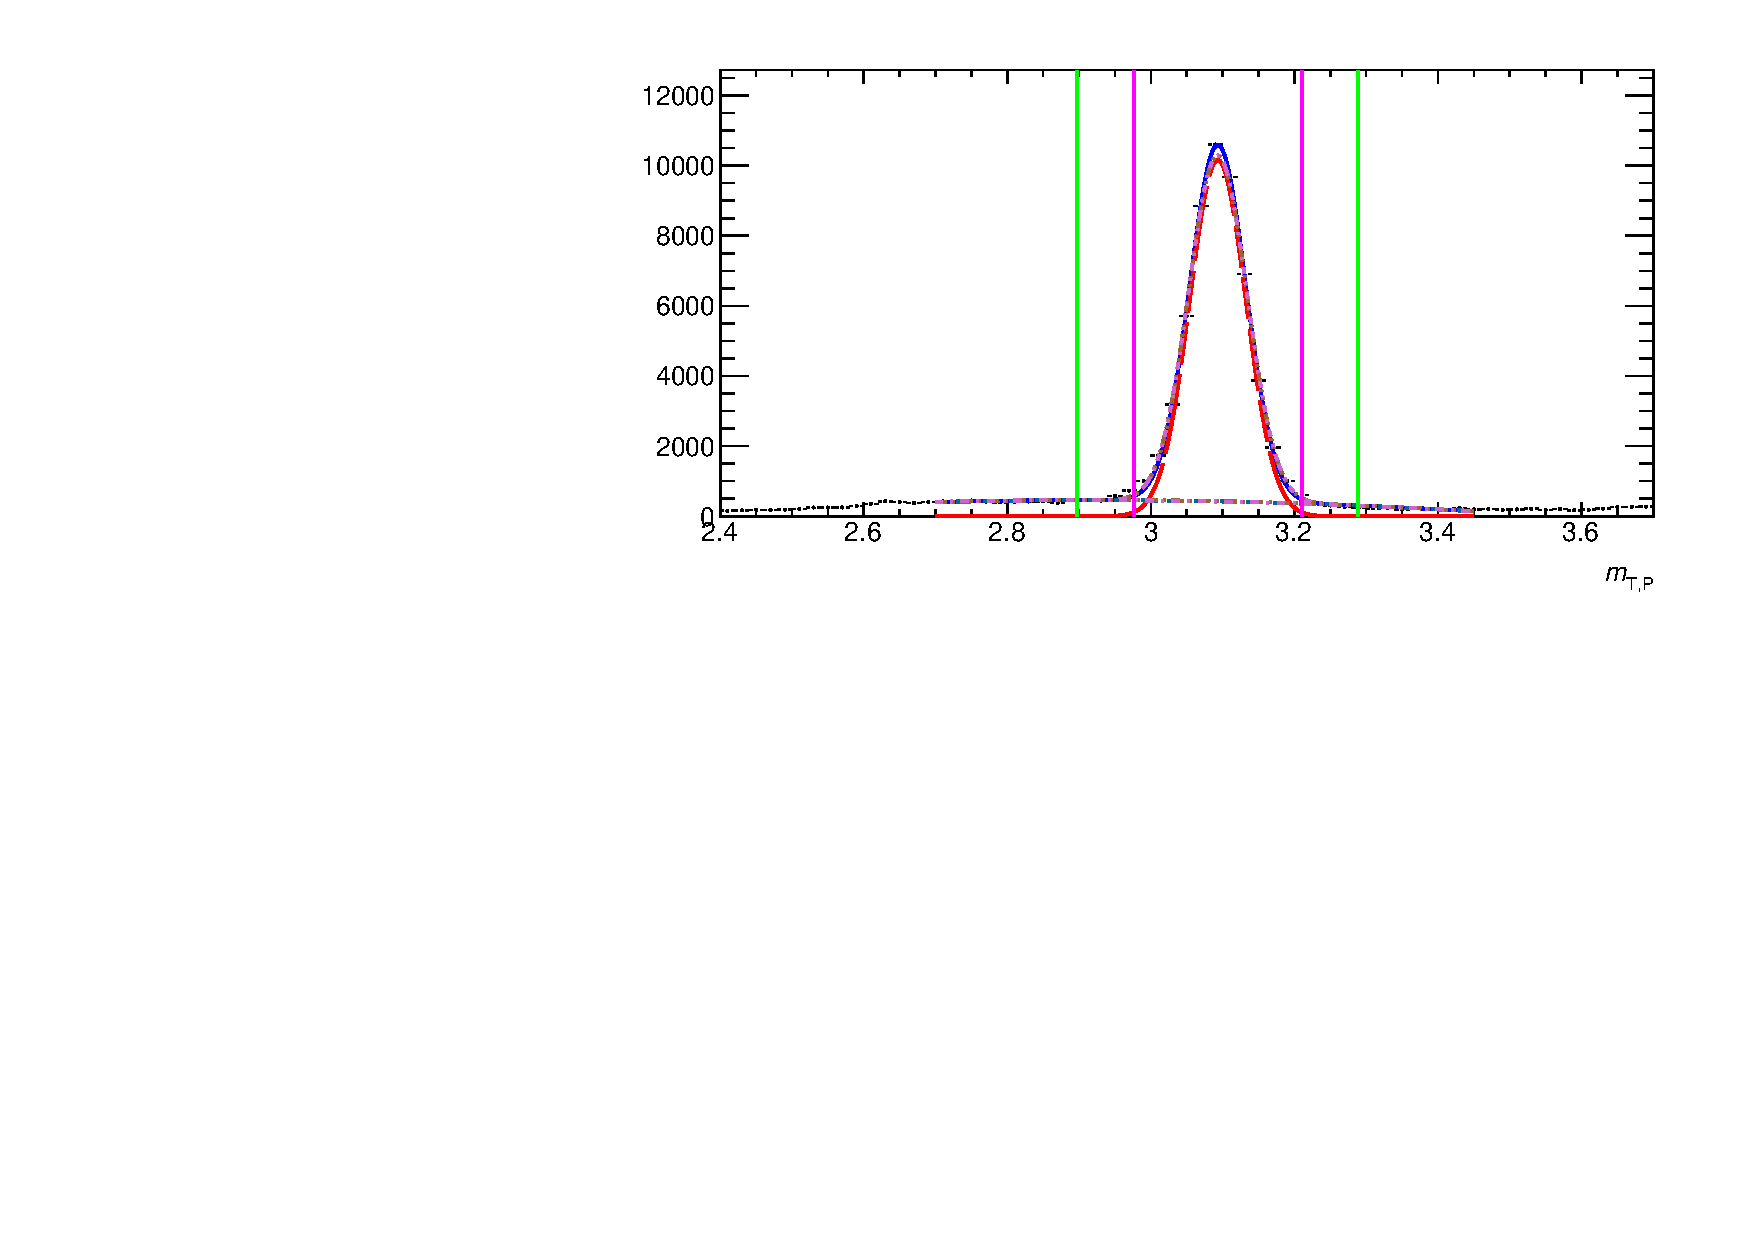
\includegraphics[width=\textwidth]{PartCalibration2012/Plots/Kinematics/Data_InvMass_pt_5_6_barrel_muonprobe.pdf}
      \caption{Muon probe level}\label{fig:CalibrationInvMassMuonProbe}
    \end{subfigure}

    \begin{subfigure}[b]{0.80\textwidth}
      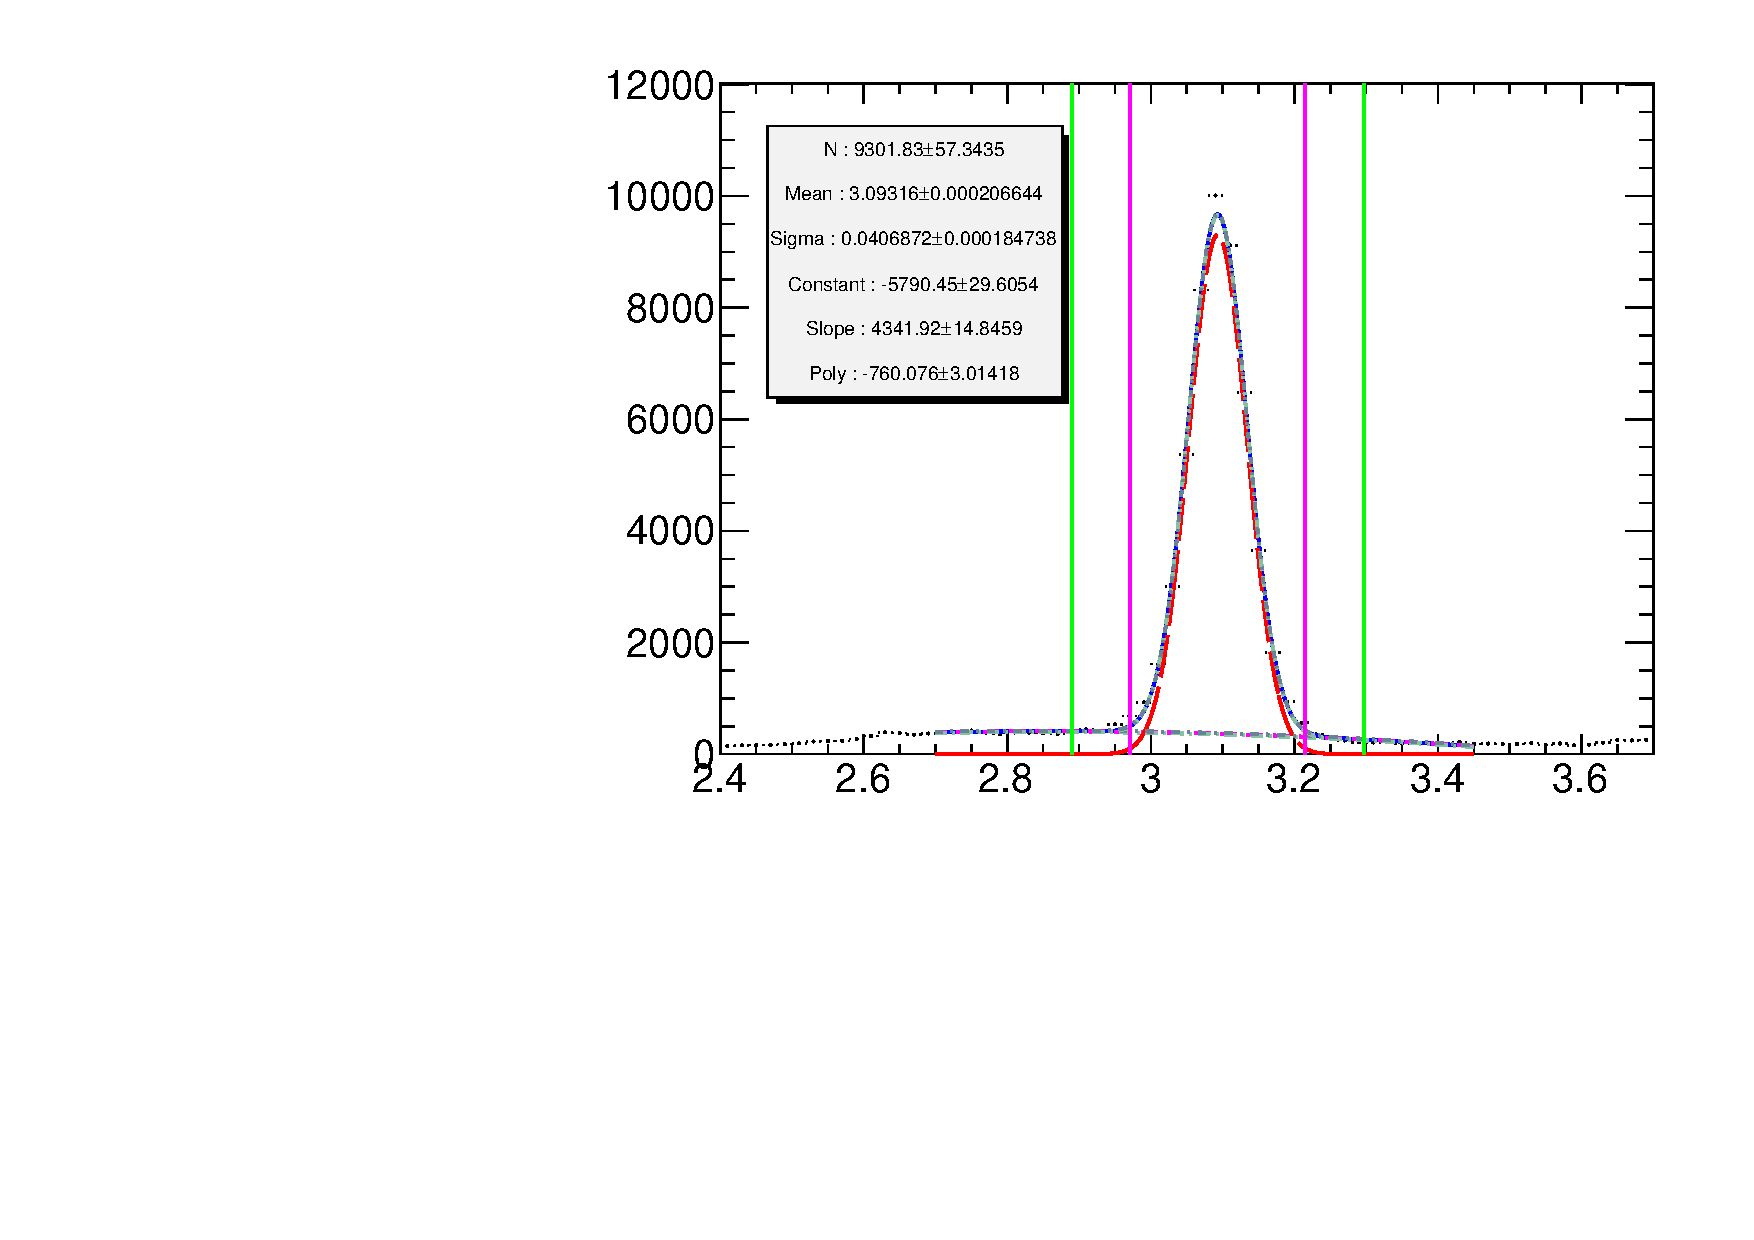
\includegraphics[width=\textwidth]{PartCalibration2012/Plots/Kinematics/Data_InvMass_pt_5_6_barrel_smt.pdf}
      \caption{SMT probe level}\label{fig:CalibrationInvMassSMT}
    \end{subfigure}
    \caption[Invariant mass distributions of tag and probe pairs at probe level, muon probe level, and SMT level in collision data for probes in barrel A with a \pt\ of {\SIrange[range-units=single]{5}{6}{\GeV}}.]{Invariant mass distributions of tag and probe pairs at~\subref{fig:CalibrationInvMassProbe} probe level,~\subref{fig:CalibrationInvMassMuonProbe} muon probe level, and~\subref{fig:CalibrationInvMassSMT} SMT level in collision data for probes in barrel A with a \pt\ of \SIrange[range-units=single]{5}{6}{\GeV}. Shown are all the components of the fit including: composite nominal fit (solid curve), nominal background (dashed curve), background variations (dashed-dot curves), implied \jpsi\ peak (long dashed red curve), the $3\sigma$ and $5\sigma$ integration windows used for systematics (vertical lines).}\label{fig:CalibrationFittingResult}
\end{figure}

\section{Efficiencies}\label{sec:CalibrationEfficiencies}

The efficiency is monitored as a function of a variety of kinematic variables, including the isolation, transverse momentum, azimuthal angle, and the pseudorapidity of the probe.

\subsection{The 2011 calibration}

The selection and fitting procedure used for this calibration are based on the 2011 analysis~\cite{Calibration:MattThesis}. In that calibration, the efficiencies measured exhibited no dependence on $\phi$, an asymmetric dependence on $\eta$ particularly in the forward regions of the detector, and a dependence on \pt. The scale factors were close to unity within their uncertainty across the entire $\eta$ and $\pt$ range examined as shown in Table~\ref{tab:Calibration2011SF}.

\begin{table}[bhtp]
  \centering
  \tabcolsep=0.11cm
  \ra{1.3}
  \sisetup{range-phrase=--}
  \begin{tabular}{@{}%
                    l%
                    *{5}{S[table-format=1.3(3)]}%
                    @{}}
    \toprule
    \pt\ range [\si{\GeV}]   & \multicolumn{5}{c}{Scale Factor in} \\
    \midrule
    \textbf{Side A}          & {Crack}   & {Barrel} & {Transition} & {End-cap} & {Forward} \\
    \tabin\numrange{4}{5}   & 0.974(9)  & 0.981(3) & 0.987(7)     & 0.981(3) & 0.991(5)  \\
    \tabin\numrange{5}{6}   & 0.996(8)  & 0.983(3) & 0.987(8)     & 0.988(4) & 0.980(6)  \\
    \tabin\numrange{6}{7}   & 0.990(9)  & 0.984(3) & 0.960(10)    & 0.984(5) & 0.981(6)  \\
    \tabin\numrange{7}{8}   & 0.966(13) & 0.987(4) & 0.978(8)     & 0.990(6) & 0.982(7)  \\
    \tabin\numrange{8}{10}  & 0.983(11) & 0.981(3) & 1.005(9)     & 0.988(5) & 0.954(8)  \\
    \tabin\numrange{10}{12} & 0.928(19) & 0.979(4) & 1.002(9)     & 0.991(6) & 0.984(11) \\
    \midrule
    \textbf{Side C}          & {Crack}   & {Barrel} & {Transition} & {End-cap} & {Forward} \\
    \tabin\numrange{4}{5}   & 0.984(8)  & 0.978(3) & 0.992(7)     & 0.979(3) & 1.005(6)  \\
    \tabin\numrange{5}{6}   & 0.992(7)  & 0.991(2) & 0.982(9)     & 0.986(4) & 1.012(7)  \\
    \tabin\numrange{6}{7}   & 0.989(8)  & 0.981(3) & 0.980(8)     & 0.990(5) & 1.003(10) \\
    \tabin\numrange{7}{8}   & 0.931(17) & 0.983(3) & 0.970(53)    & 0.985(6) & 1.047(10) \\
    \tabin\numrange{8}{10}  & 0.981(17) & 0.987(3) & 0.968(9)     & 0.990(5) & 1.100(8)  \\
    \tabin\numrange{10}{12} & 0.974(15) & 0.976(4) & 0.970(11)    & 1.002(6) & 1.083(10) \\
    \bottomrule
  \end{tabular}
  \caption[Data/MC Scale Factors for 2011 Data in all five regions of the detector as a function of \pt.]{Data/MC Scale Factors for 2011 Data in all five regions of the detector as a function of \pt. The uncertainties include systematic and statistical components as described in~\cite{Calibration:MattThesis}.}\label{tab:Calibration2011SF}
\end{table}

\subsection{Efficiency binning}\label{sec:CalibrationBinning}
\sisetup{range-phrase=--}
The binning in most variables is governed by the amount of data required to produce stable, good quality fits. The binning in pseudorapidity, summarized in Table~\ref{tab:CalibrationEtaRegions}, corresponds with different regions of the ATLAS detector and differentiates between the positive and negative sides. The chosen \pt\ binning is shown in Table~\ref{tab:Calibration2012SF}.

\begin{table}[thbp]
  \centering
  \begin{tabular}{@{}lc@{}}
    \toprule
    Name       & $|\eta|$ range \\
    \midrule
    Crack      & \numrange{0.0}{0.1} \\
    Barrel     & \numrange{0.1}{1.1} \\
    Transition & \numrange{1.1}{1.3} \\
    End-cap    & \numrange{1.3}{2.0} \\
    Forward    & \numrange{2.0}{2.5} \\
    \bottomrule
  \end{tabular}
  \caption{Pseudorapidity regions of the ATLAS detector.}\label{tab:CalibrationEtaRegions}
\end{table}

\section{Results}

The reconstruction and \xsm\ tagging efficiencies are presented in the following pages as a function of $\eta$, $\phi$ and \pt. The STACO CB reconstruction efficiencies and scale factors as measured in side A and C of the detector are shown in Figure~\ref{fig:RecoEffSideA} and Figure~\ref{fig:RecoEffSideC} respectively. The efficiencies exhibit a strong dependence on transverse momentum and pseudorapidity.

The reconstruction efficiency for muons in the crack region appears to suffer from low data particularly in the high-\pt\ range, this is expected due to the MS being only partially equipped in the region around $\eta=0$. In the transition region the MS coverage in $\phi$ is not uniform due to some chambers not being installed.

\begin{figure}[htbp]
  \centering
    \begin{subfigure}[b]{0.45\textwidth}
      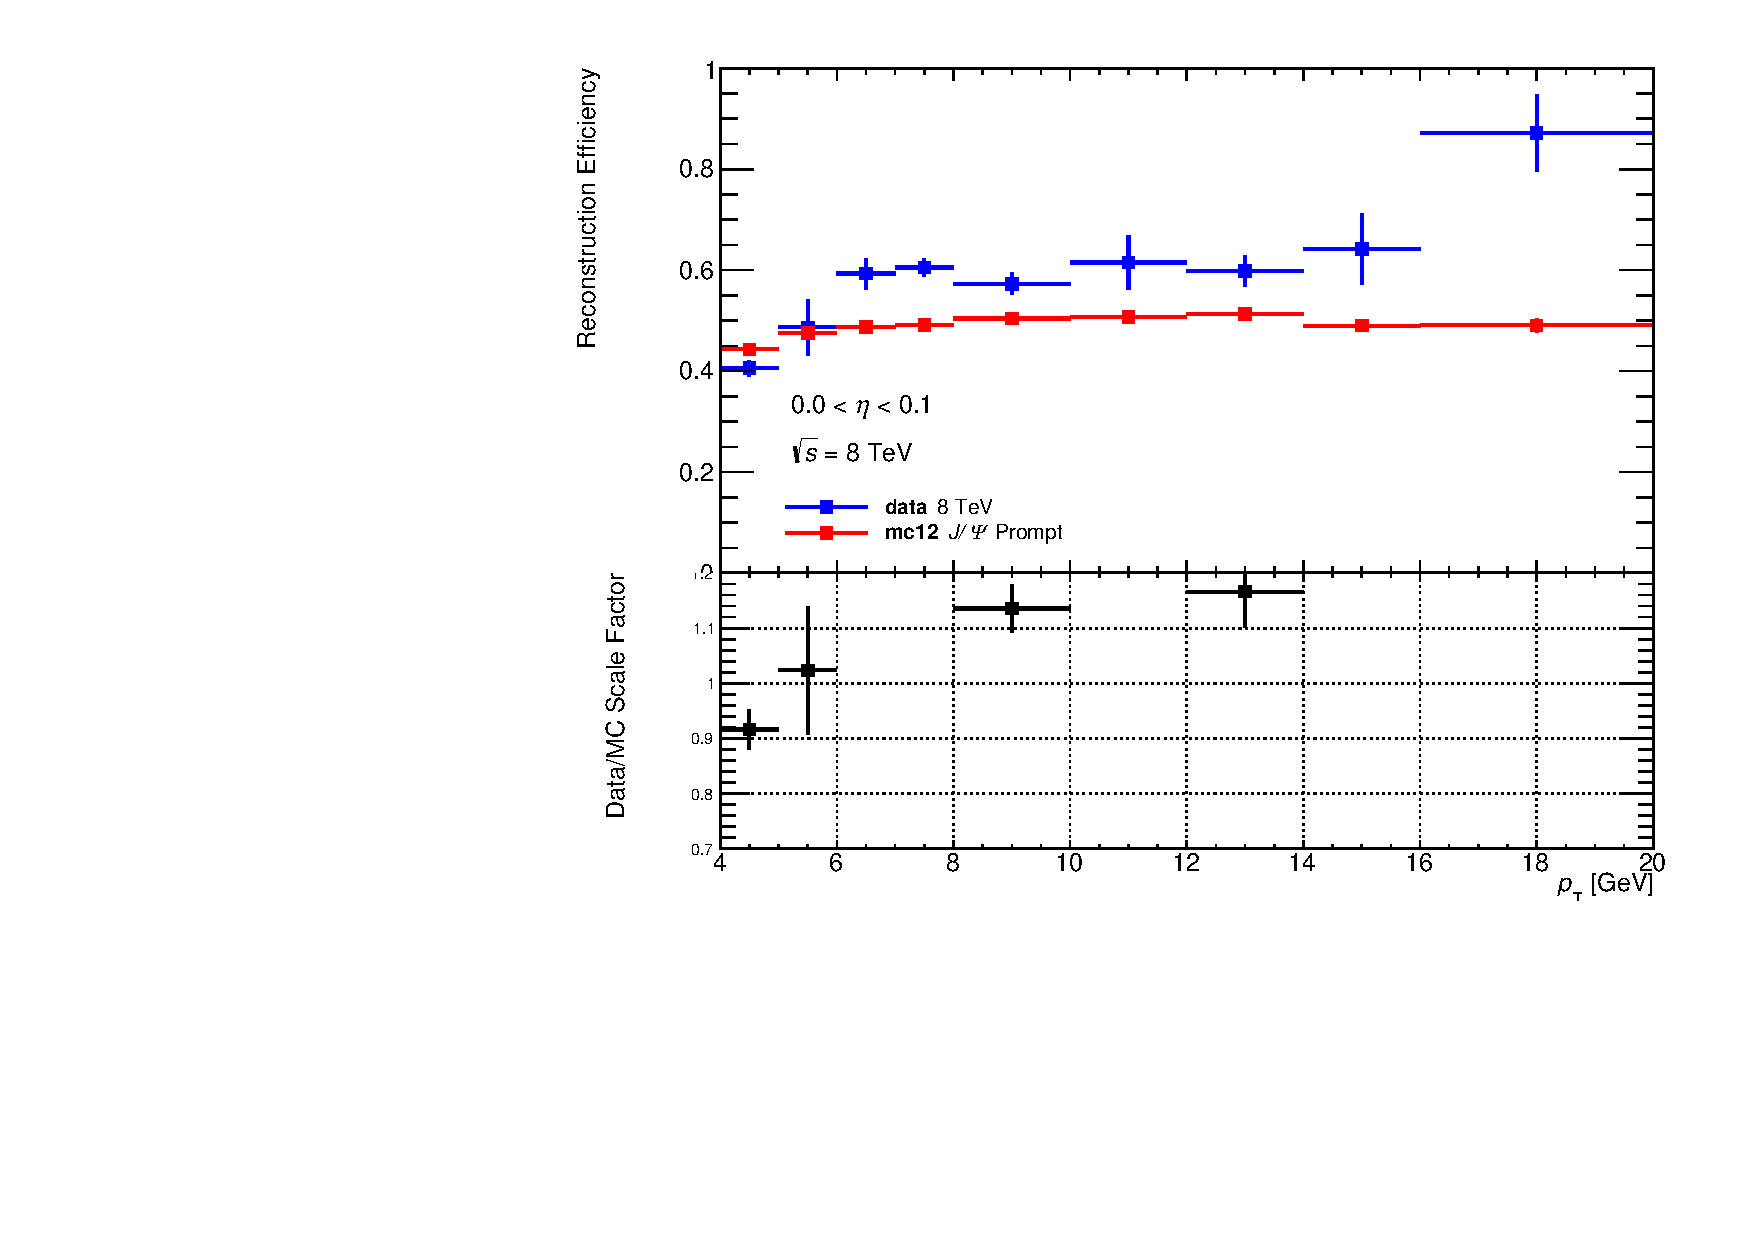
\includegraphics[width=\textwidth]{PartCalibration2012/Plots/SFPlots/Crack_A_reco.pdf}
      \caption{Crack A.}\label{fig:CalibrationRecoSFCrackA}
    \end{subfigure}
    \hfill
    \begin{subfigure}[b]{0.45\textwidth}
      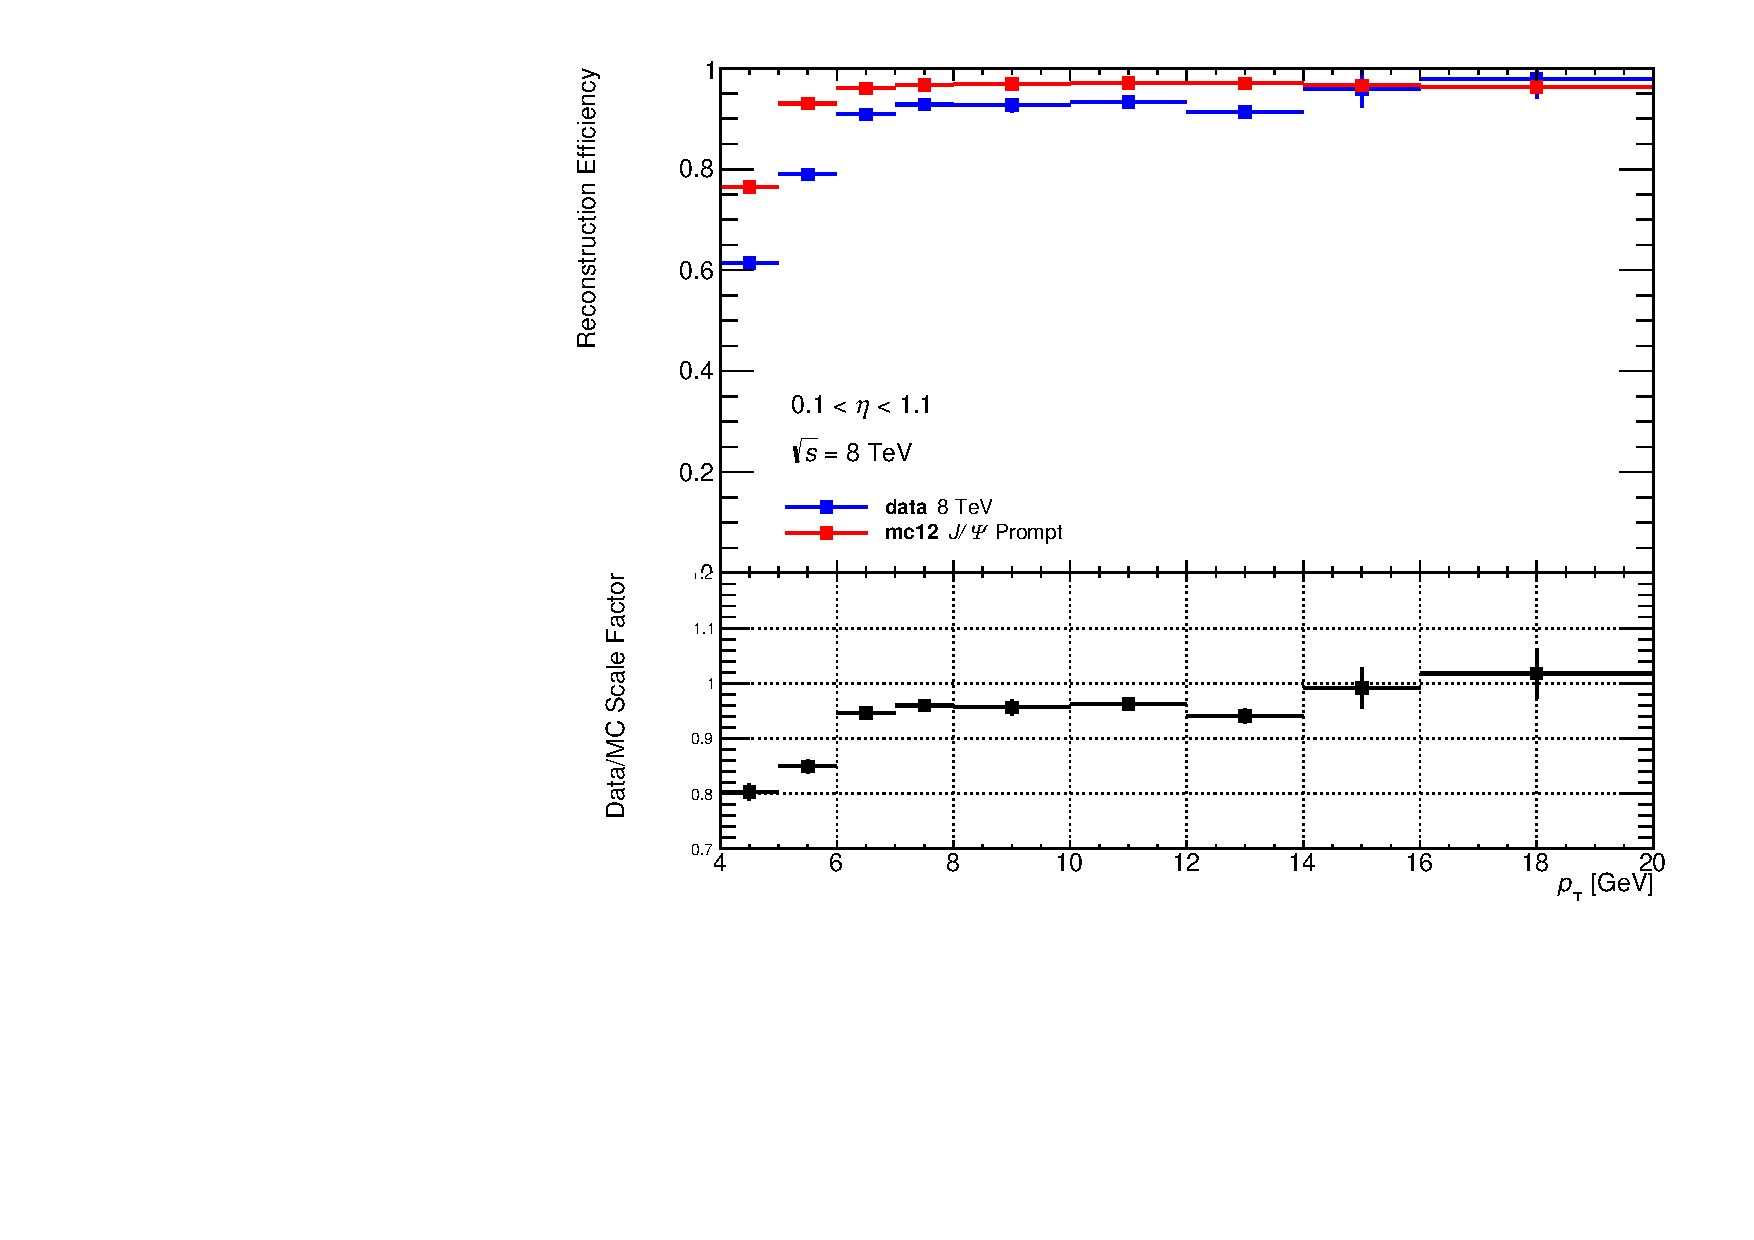
\includegraphics[width=\textwidth]{PartCalibration2012/Plots/SFPlots/Barrel_A_reco.pdf}
      \caption{Barrel A.}\label{fig:CalibrationRecoSFBarrelA}
    \end{subfigure}

    \begin{subfigure}[b]{0.45\textwidth}
      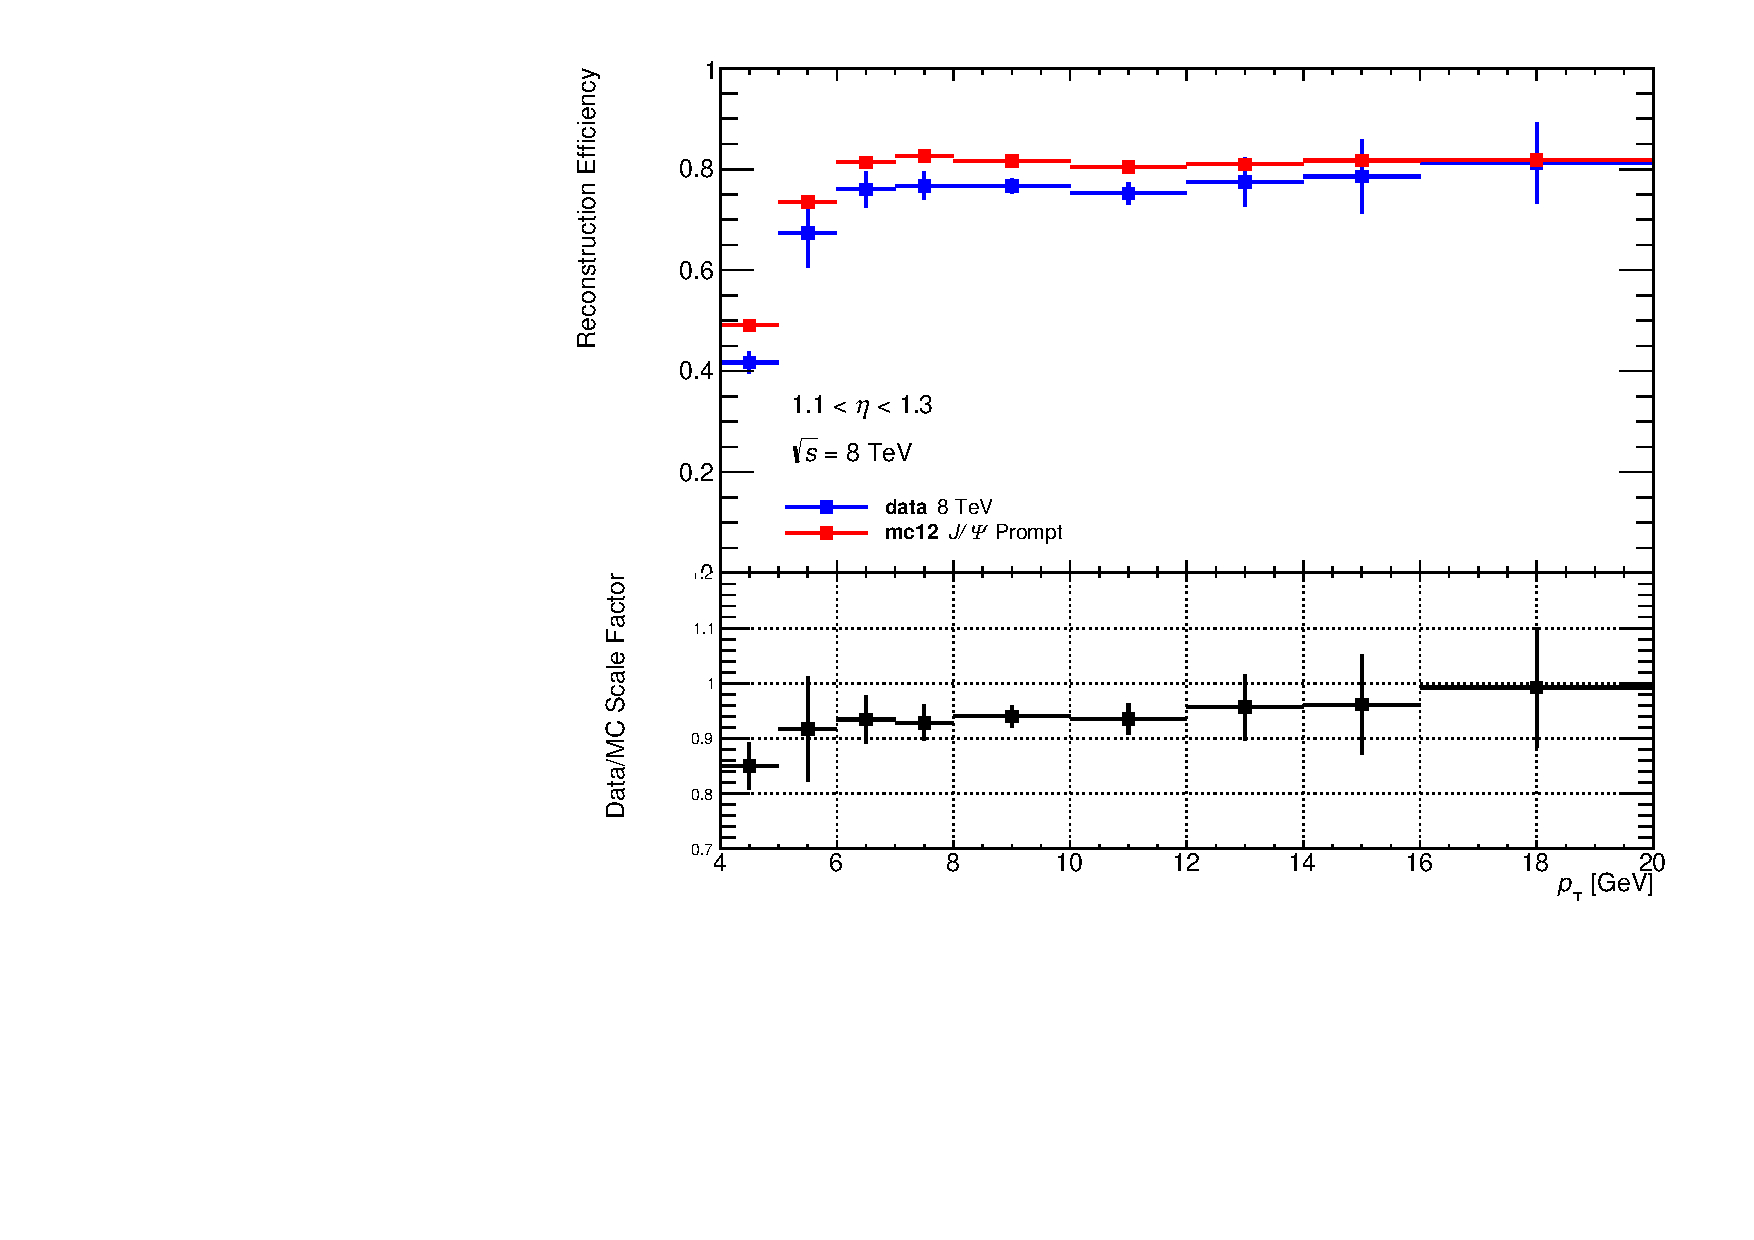
\includegraphics[width=\textwidth]{PartCalibration2012/Plots/SFPlots/Transition_A_reco.pdf}
      \caption{Transition A.}\label{fig:CalibrationRecoSFTransitionA}
    \end{subfigure}
    \hfill
    \begin{subfigure}[b]{0.45\textwidth}
      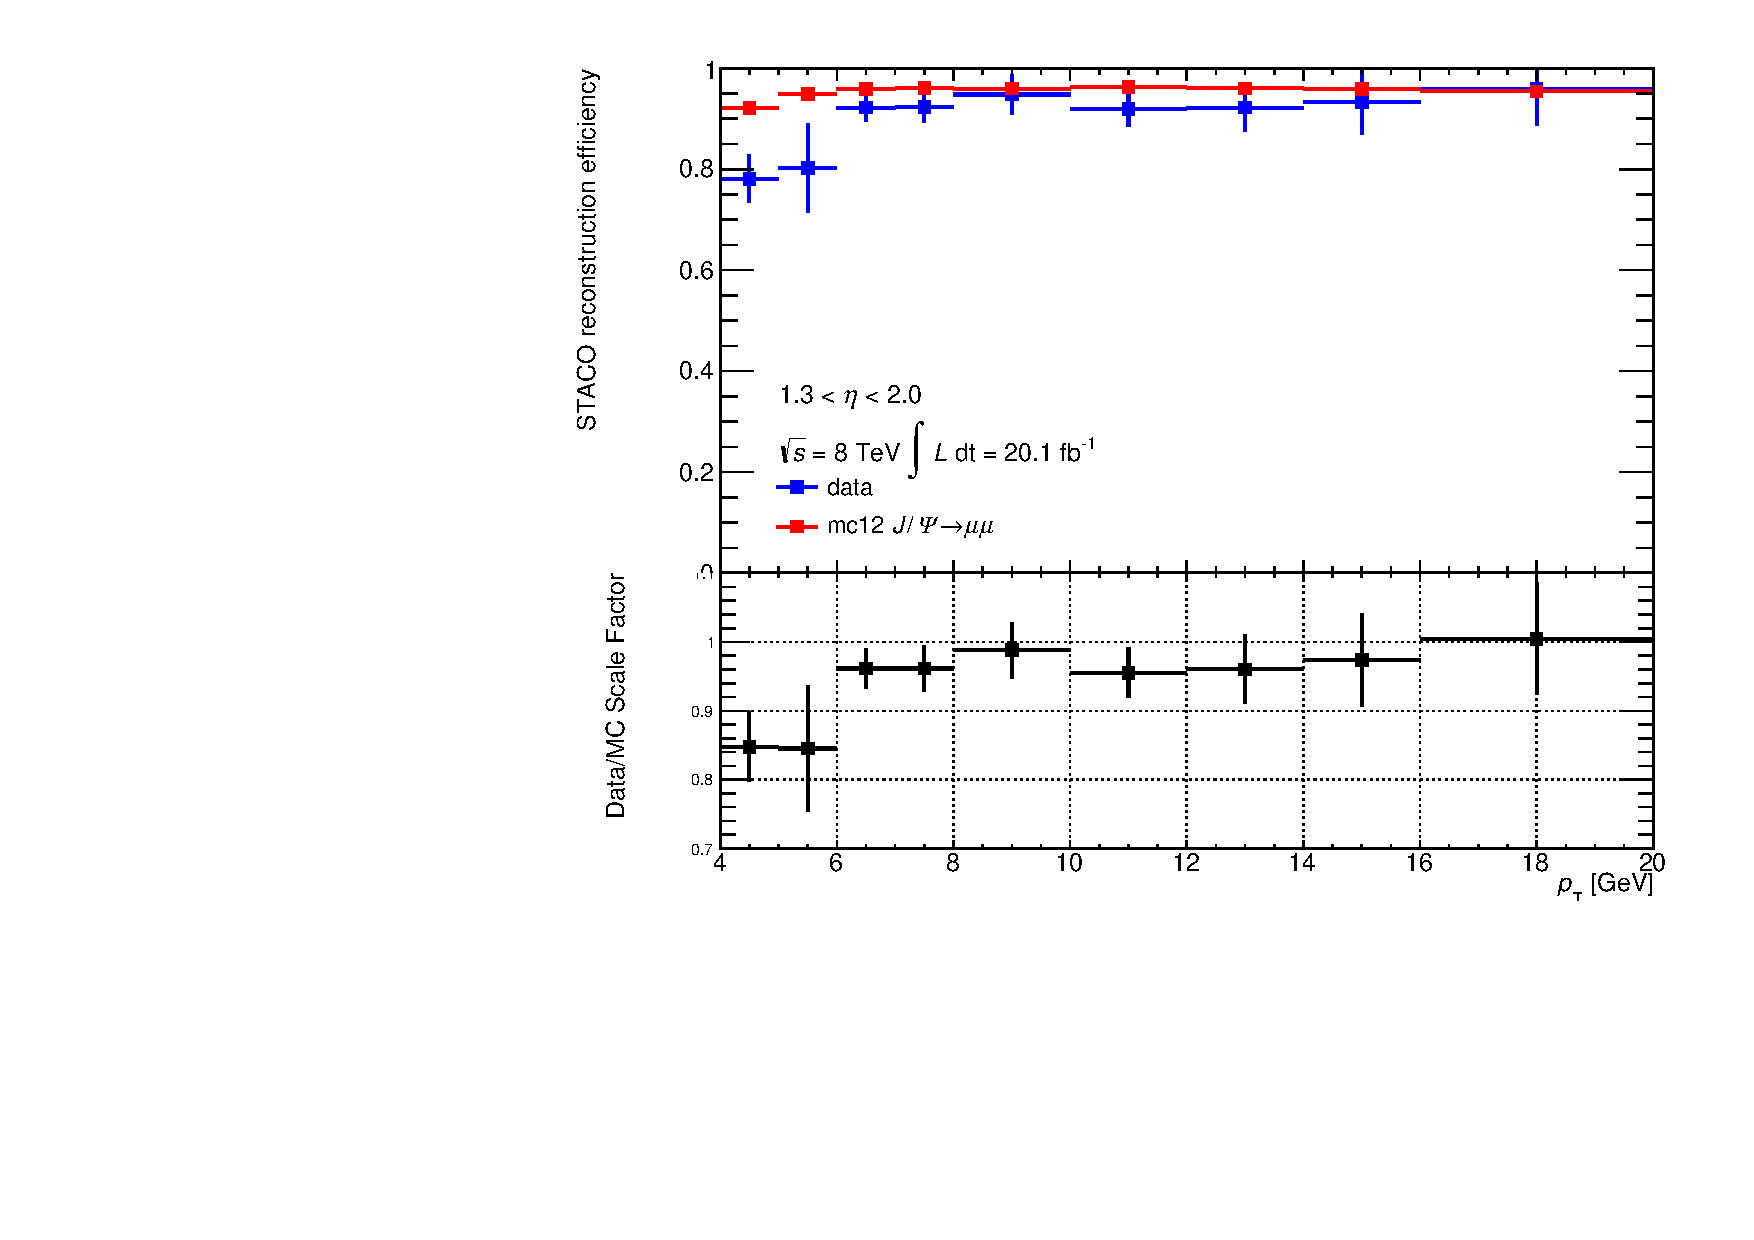
\includegraphics[width=\textwidth]{PartCalibration2012/Plots/SFPlots/Endcap_A_reco.pdf}
      \caption{End-cap A.}\label{fig:CalibrationRecoSFEndcapA}
    \end{subfigure}

    \begin{subfigure}[b]{0.45\textwidth}
      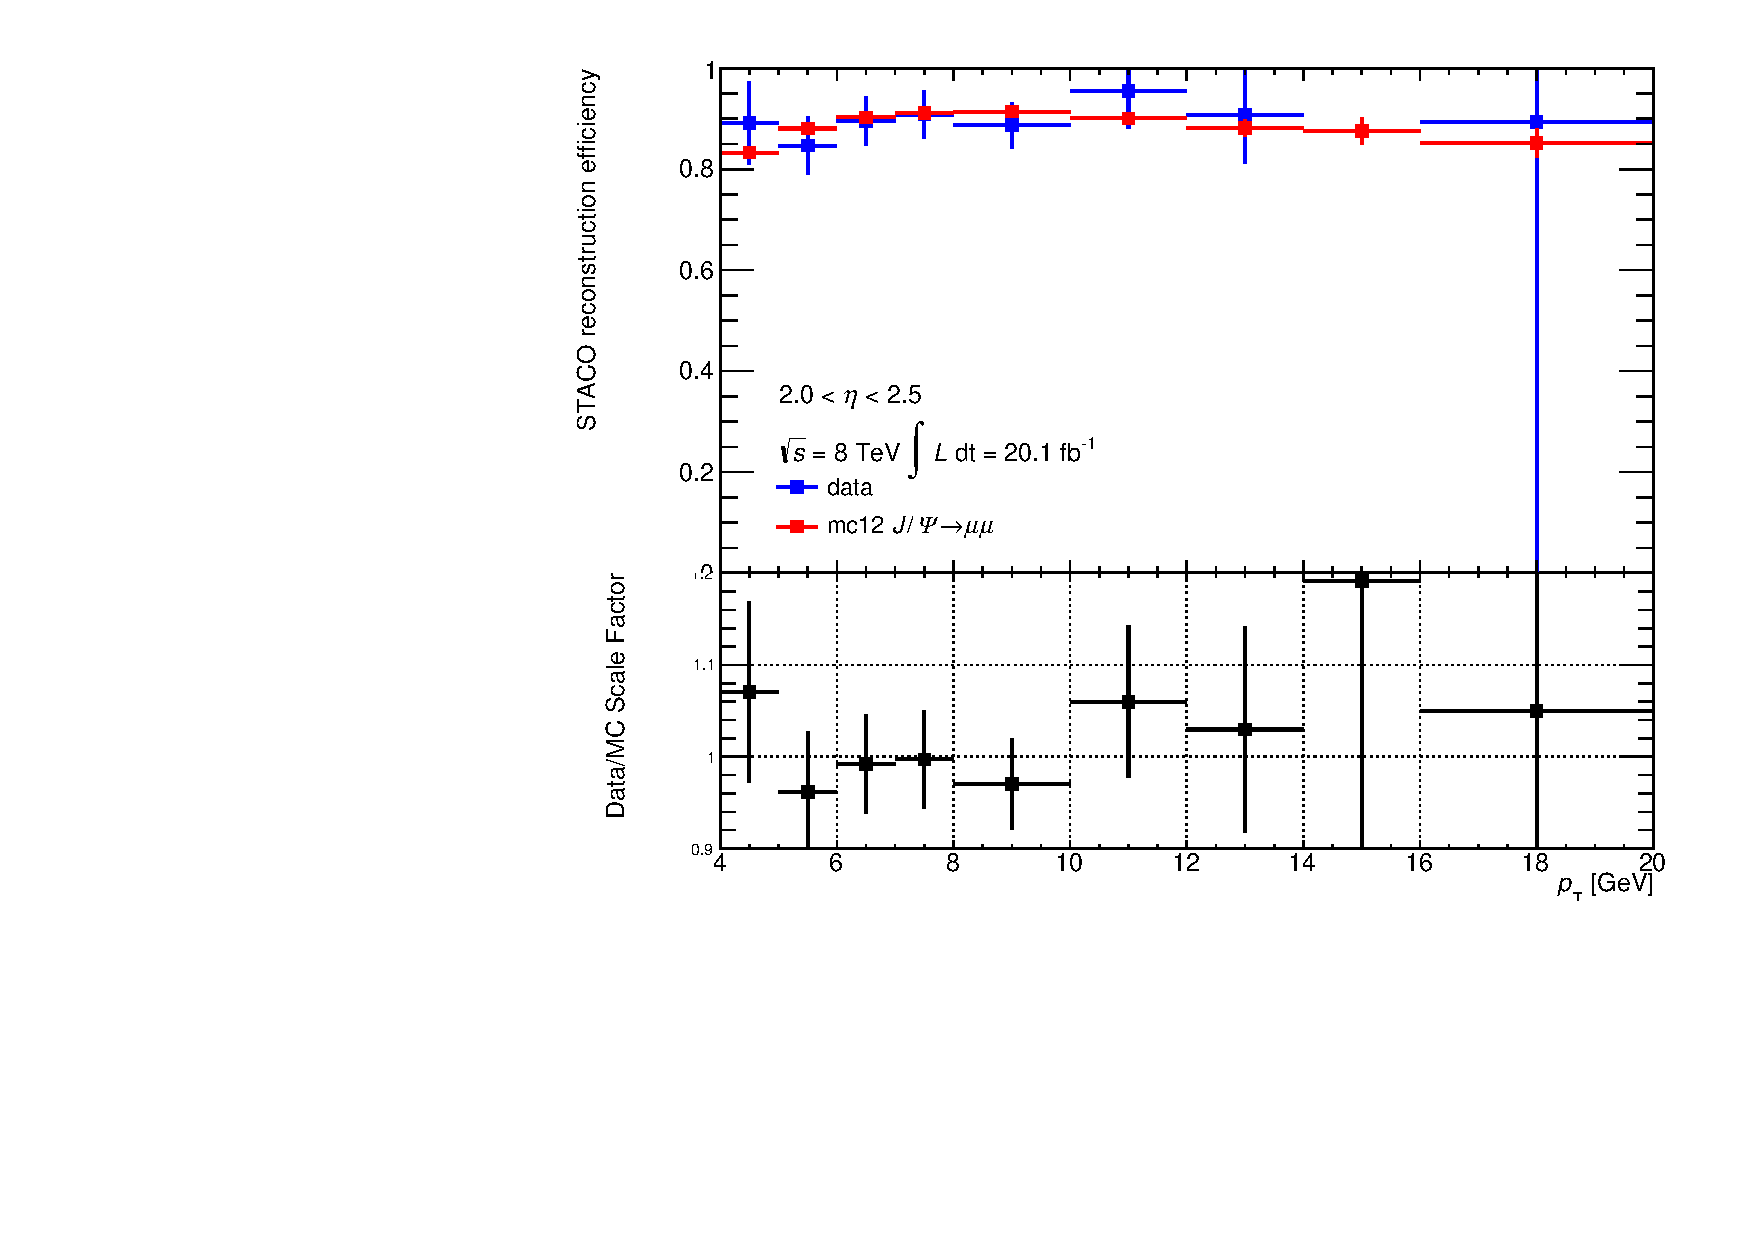
\includegraphics[width=\textwidth]{PartCalibration2012/Plots/SFPlots/Forward_A_reco.pdf}
      \caption{Forward A.}\label{fig:CalibrationRecoSFForwardA}
    \end{subfigure}
    \caption{Distribution of the STACO CB reconstruction efficiency as measured in data and MC, and the associated scale factor as a function of the probe \pt\ measured in side A for all detector regions.}\label{fig:RecoEffSideA}
\end{figure}

\begin{figure}[htbp]
  \centering
    \begin{subfigure}[b]{0.45\textwidth}
      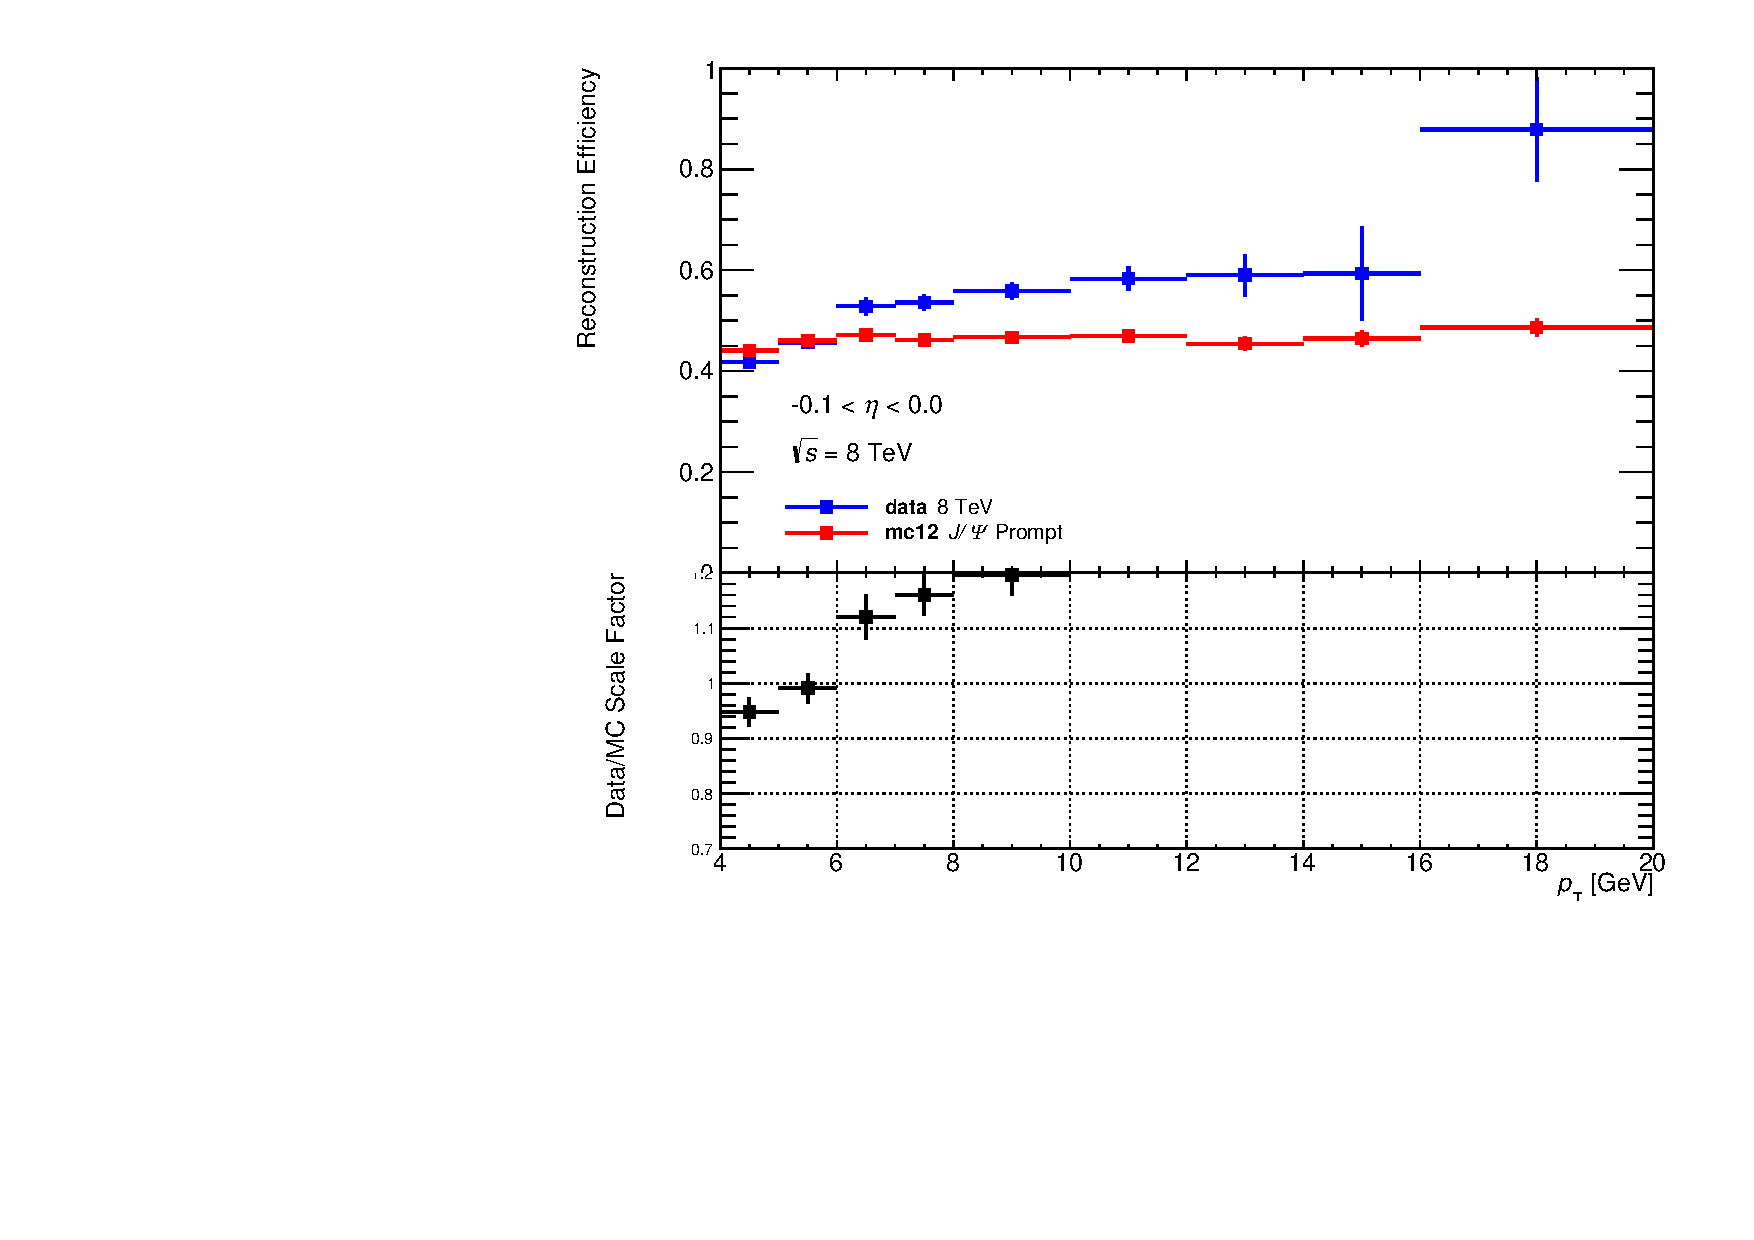
\includegraphics[width=\textwidth]{PartCalibration2012/Plots/SFPlots/Crack_C_reco.pdf}
      \caption{Crack C.}\label{fig:CalibrationRecoSFCrackC}
    \end{subfigure}
    \hfill
    \begin{subfigure}[b]{0.45\textwidth}
      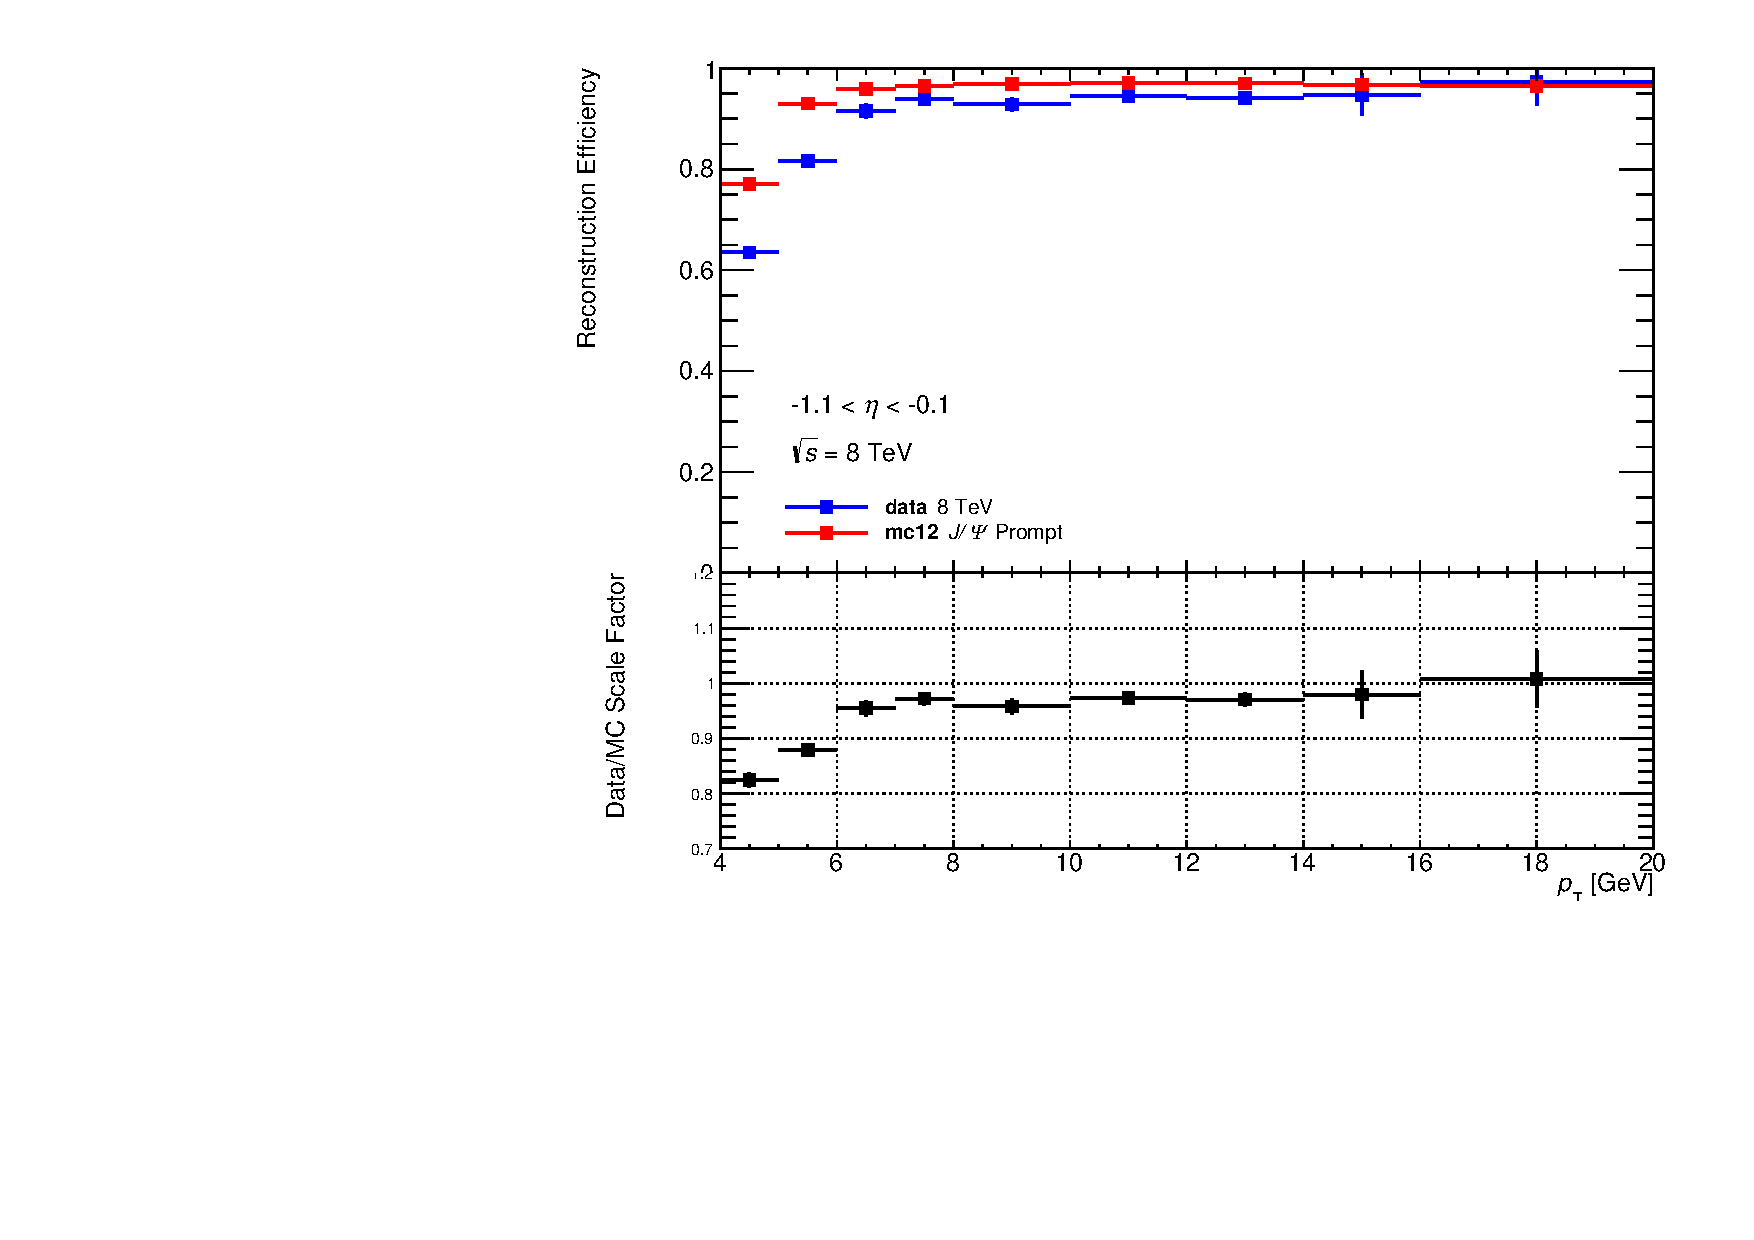
\includegraphics[width=\textwidth]{PartCalibration2012/Plots/SFPlots/Barrel_C_reco.pdf}
      \caption{Barrel C.}\label{fig:CalibrationRecoSFBarrelC}
    \end{subfigure}

    \begin{subfigure}[b]{0.45\textwidth}
      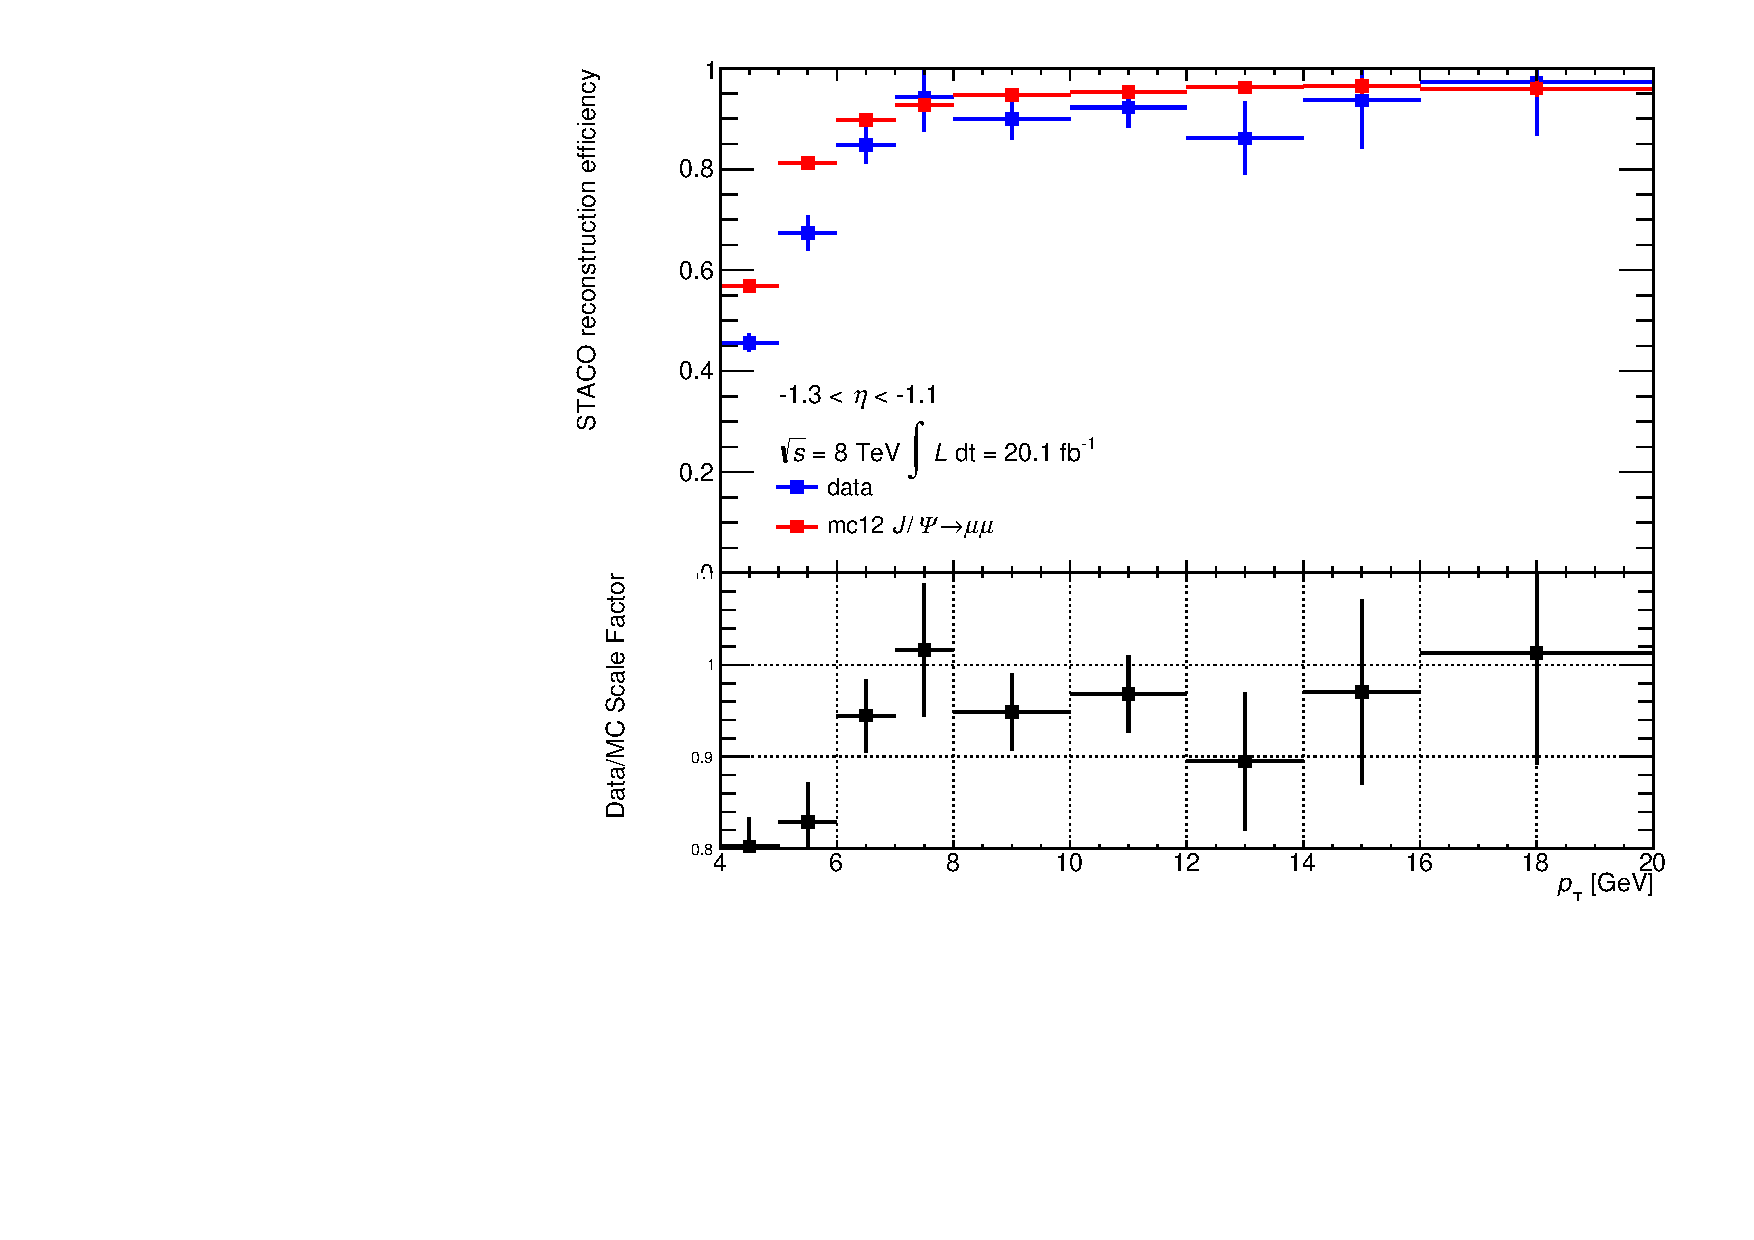
\includegraphics[width=\textwidth]{PartCalibration2012/Plots/SFPlots/Transition_C_reco.pdf}
      \caption{Transition C.}\label{fig:CalibrationRecoSFTransitionC}
    \end{subfigure}
    \hfill
    \begin{subfigure}[b]{0.45\textwidth}
      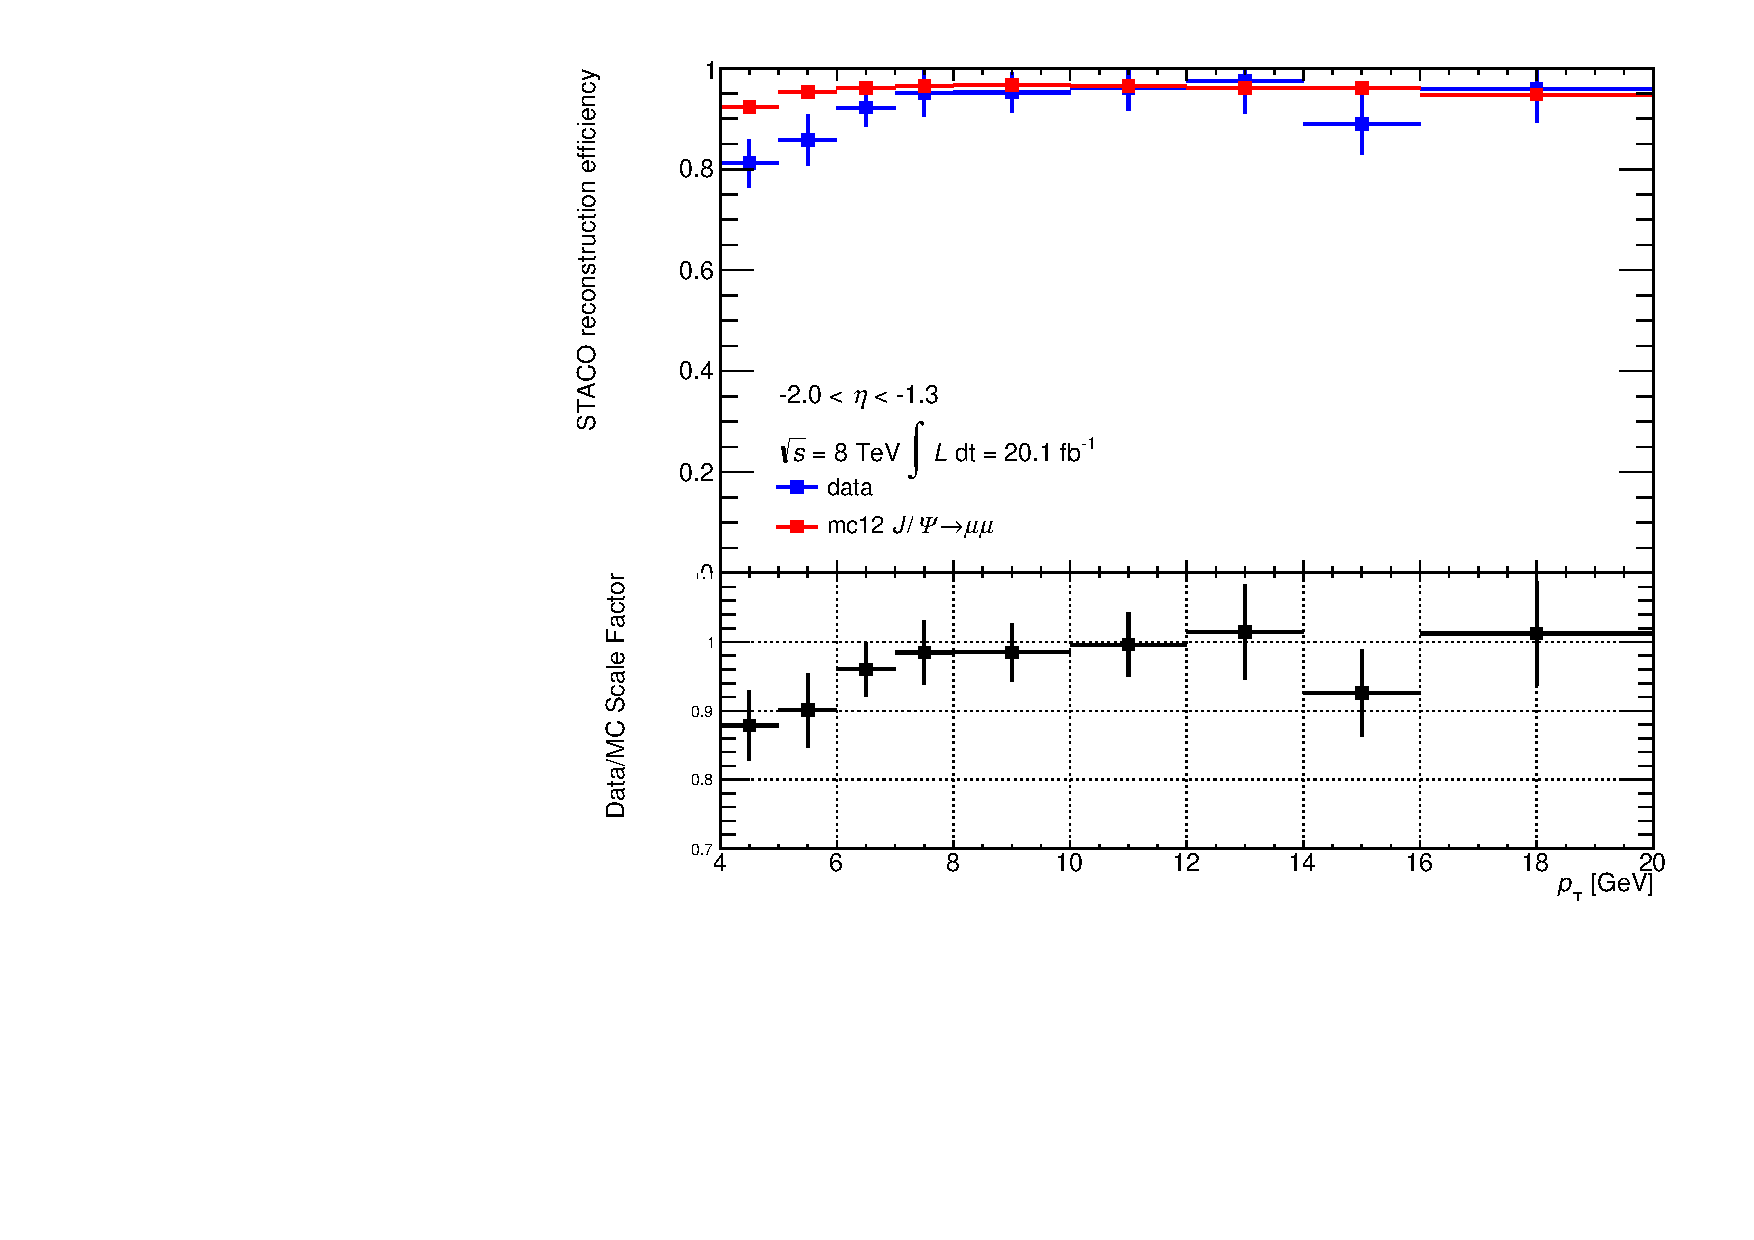
\includegraphics[width=\textwidth]{PartCalibration2012/Plots/SFPlots/Endcap_C_reco.pdf}
      \caption{End-cap C.}\label{fig:CalibrationRecoSFEndcapC}
    \end{subfigure}

    \begin{subfigure}[b]{0.45\textwidth}
      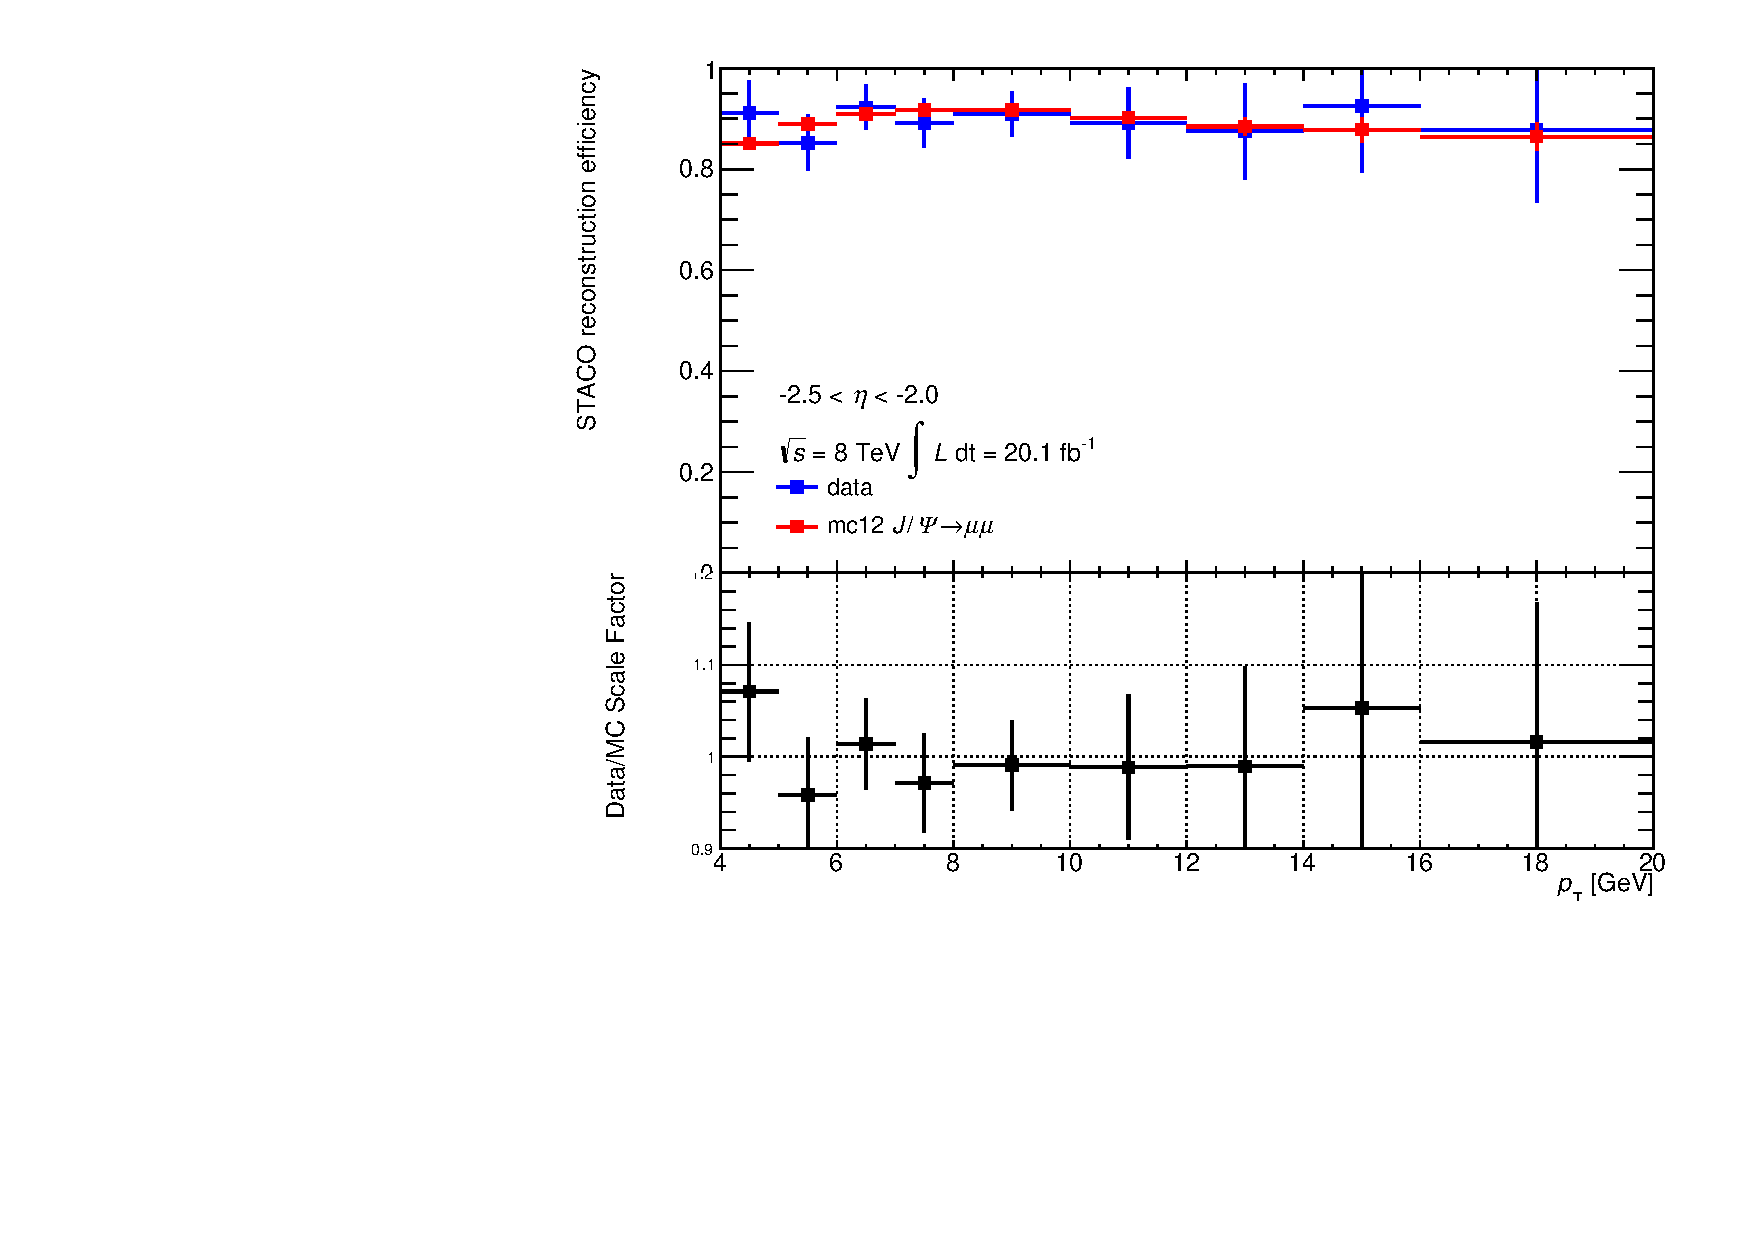
\includegraphics[width=\textwidth]{PartCalibration2012/Plots/SFPlots/Forward_C_reco.pdf}
      \caption{Forward C.}\label{fig:CalibrationRecoSFForwardC}
    \end{subfigure}
    \caption{Distribution of the STACO CB reconstruction efficiency as measured in data and MC, and the associated scale factor as a function of the probe \pt\ measured in side C for all detector regions.}\label{fig:RecoEffSideC}
\end{figure}

The \xsm\ tagging efficiency exhibits an asymmetric dependence on the muon probe pseudorapidity, but no dependence on the azimuthal angle $\phi$ (Figure~\ref{fig:CalibrationAngularResults}). As expected, there is a strong dependence on the transverse momentum of the muon probe (Figure~\ref{fig:CalibrationMomentumResults}). As in the 2011 analysis it was decided to bin the SF as a function of \pt\ and $\eta$, distinguishing between side A and C of the detector. The scale factor and efficiency distributions are presented in the next pages for the crack region (Figure~\ref{fig:CalibrationScaleFactorCrack}), the barrel region (Figure~\ref{fig:CalibrationScaleFactorBarrel}), the transition region (Figure~\ref{fig:CalibrationScaleFactorTransition}), the endcap region (Figure~\ref{fig:CalibrationScaleFactorEndcap}), and the forward region (Figure~\ref{fig:CalibrationScaleFactorForward}).

% SF vs Eta, Phi
\begin{figure}[htbp]
  \centering
  \begin{subfigure}[b]{0.75\textwidth}
      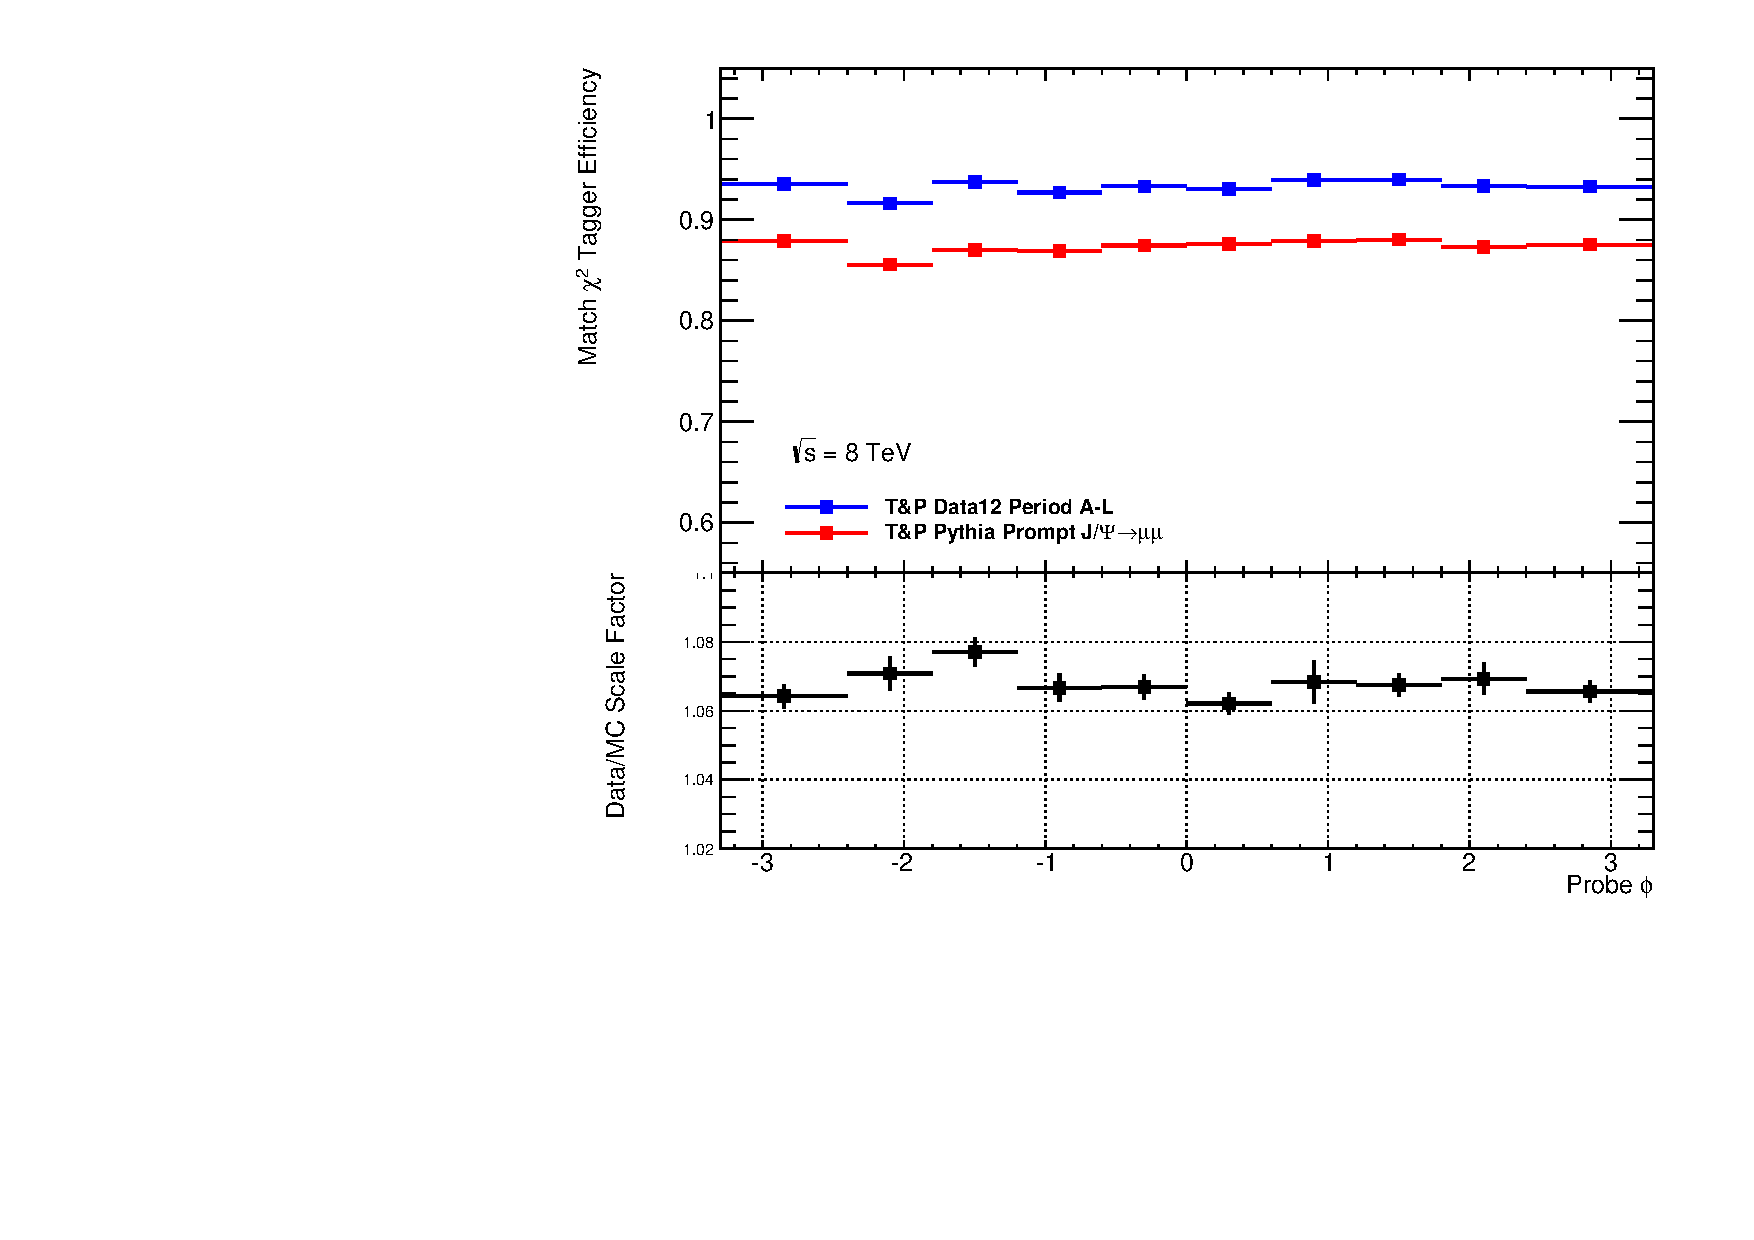
\includegraphics[width=\textwidth]{PartCalibration2012/Plots/SFPlots/phi_smt.pdf}
      \caption{\xsm\ efficiency and scale factor as a function of the azimuthal angle $\phi$ of the probe muon.}\label{fig:CalibrationPhi}
  \end{subfigure}

  \begin{subfigure}[b]{0.75\textwidth}
      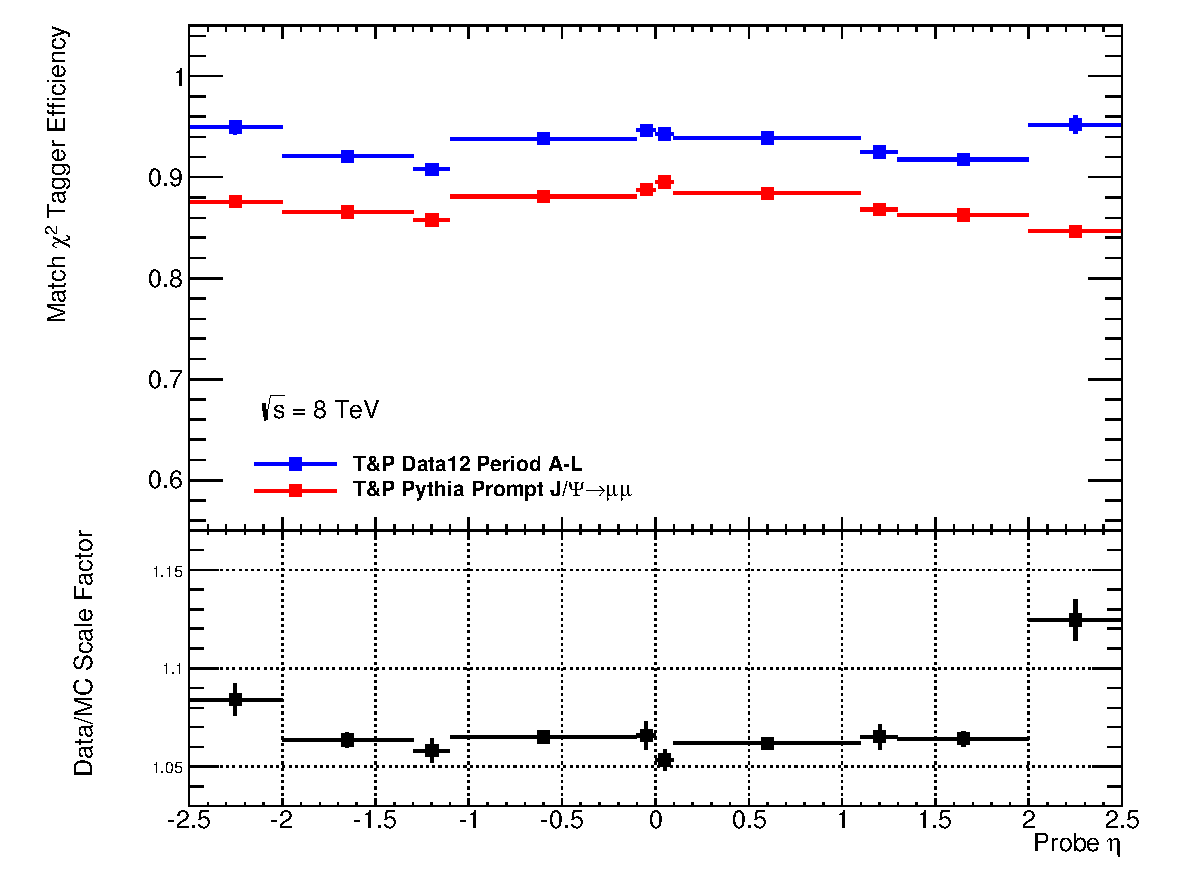
\includegraphics[width=\textwidth]{PartCalibration2012/Plots/SFPlots/eta_smt.pdf}
      \caption{\xsm\ efficiency and scale factor as a function of the pseudorapidity $\eta$ of the probe muon.}\label{fig:CalibrationEta}
  \end{subfigure}
  \caption[Distribution of the \xsm\ efficiency as measured in data and MC, and the associated scale factor with respect to the azimuthal angle $\phi$ and the pseudorapidity $\eta$ of the muon probe.]{Distribution of the \xsm\ efficiency as measured in data and MC, and the associated scale factor with respect to the~\subref{fig:CalibrationPhi} azimuthal angle $\phi$ and~\subref{fig:CalibrationEta} the pseudorapidity $\eta$ of the muon probe.}\label{fig:CalibrationAngularResults}
\end{figure}

% SF vs PT
\begin{figure}[htbp]
  \centering
    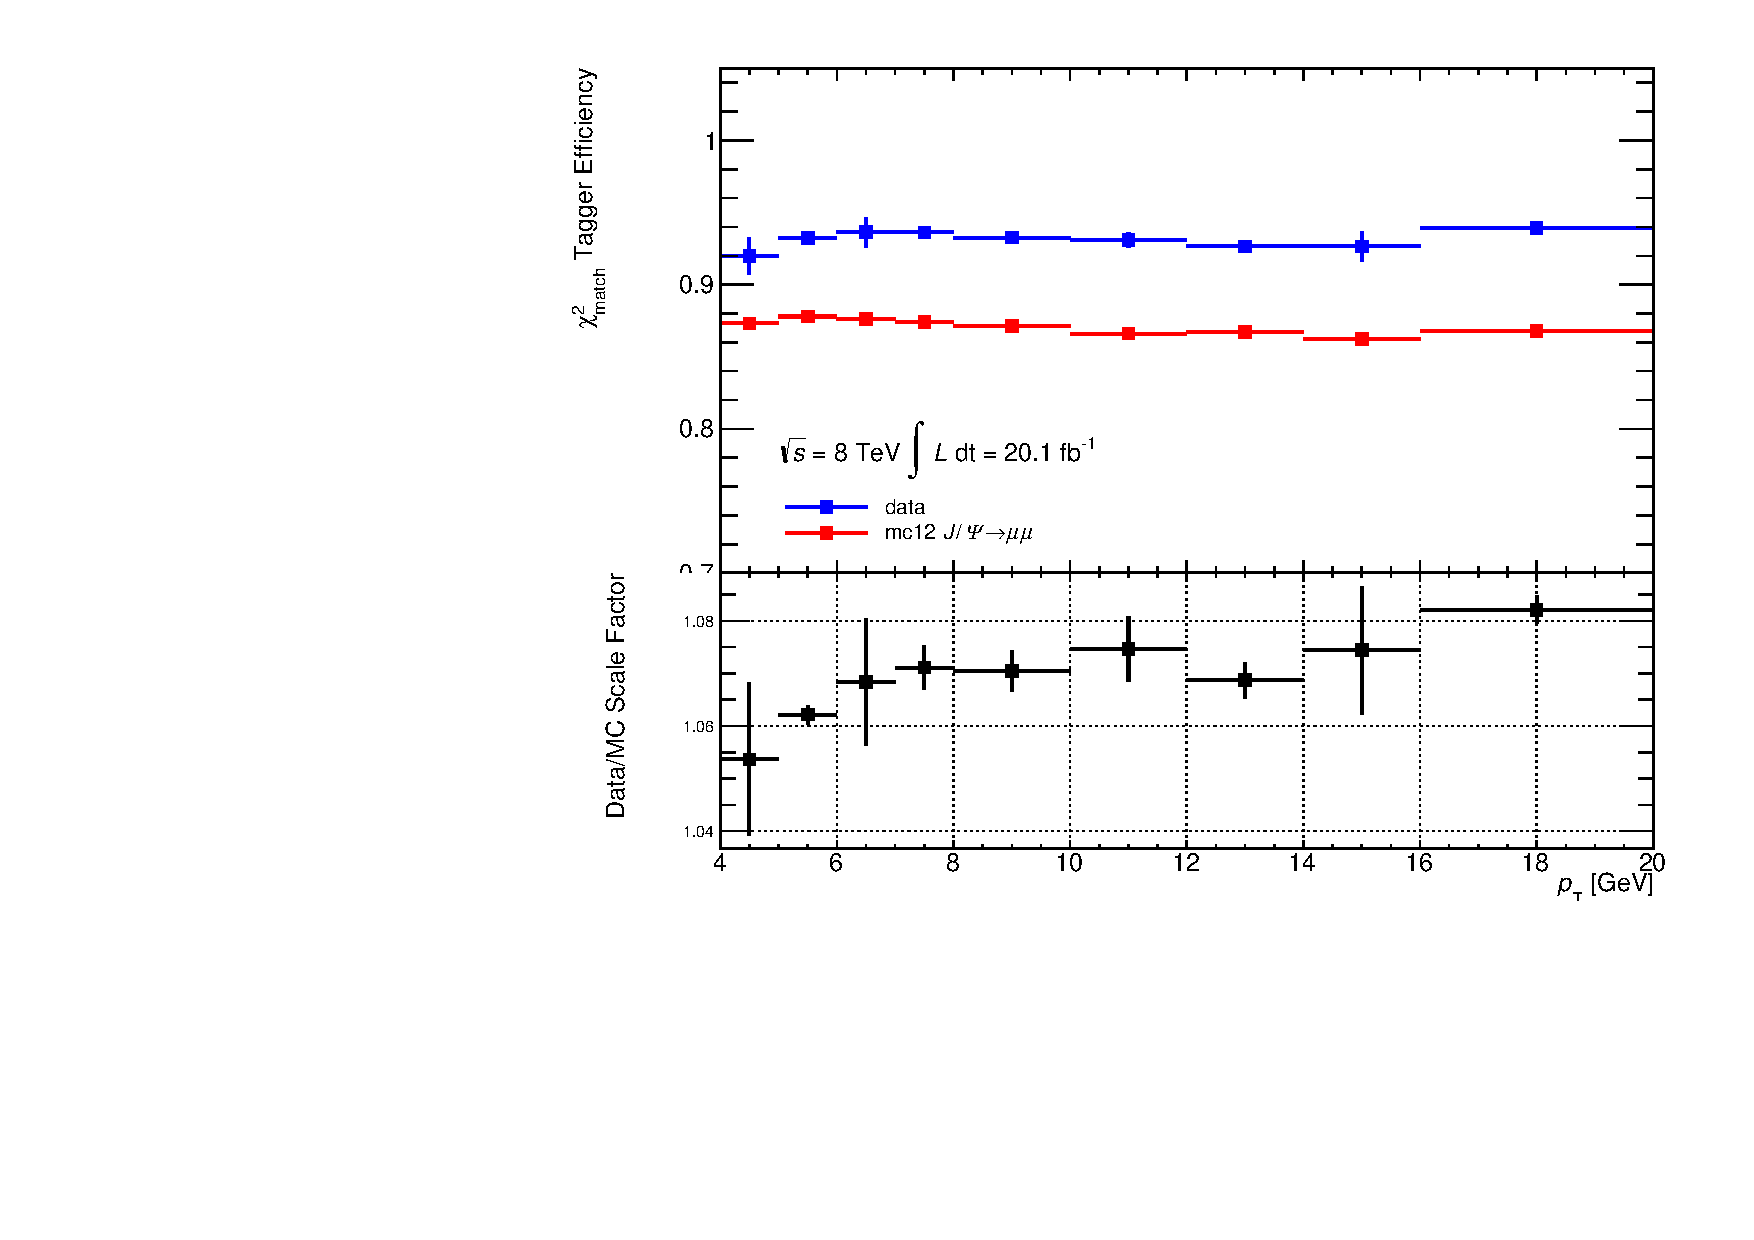
\includegraphics[width=0.75\textwidth]{PartCalibration2012/Plots/SFPlots/pt_smt.pdf}
    \caption{Distribution of the \xsm\ efficiency as measured in data and MC, and the associated scale factor with respect to the transverse momentum of the muon probe.}\label{fig:CalibrationMomentumResults}
\end{figure}

The SMT scale factors and their total uncertainties are summarized in Table~\ref{tab:Calibration2012SF}. As an example of the typical uncertainties obtained, the SMT efficiencies measured for muon probes with \pt\ in the range \SIrange[range-units=single]{5}{6}{\GeV} in the positive barrel region are
%
\begin{align*} 
  \epsilon_{\textrm{Data}} &= \fulleff{94.15}{0.32}{0.02}{0.10} \\
  \epsilon_{\textrm{MC}}   &= \fulleff{89.01}{0.01}{0.01}{0.07}
\end{align*}

As expected, the background uncertainty dominates in collision data while in simulation it represents the smallest source of uncertainty. The width of the \jpsi\ peak increases for forward probes, overwhelming the background distribution delimited by the trigger ``shoulders''. This is reflected in increased fit parameter uncertainties and a larger background uncertainty.

% Crack Region
\begin{figure}[htbp]
  \centering
    \begin{subfigure}[b]{0.85\textwidth}
        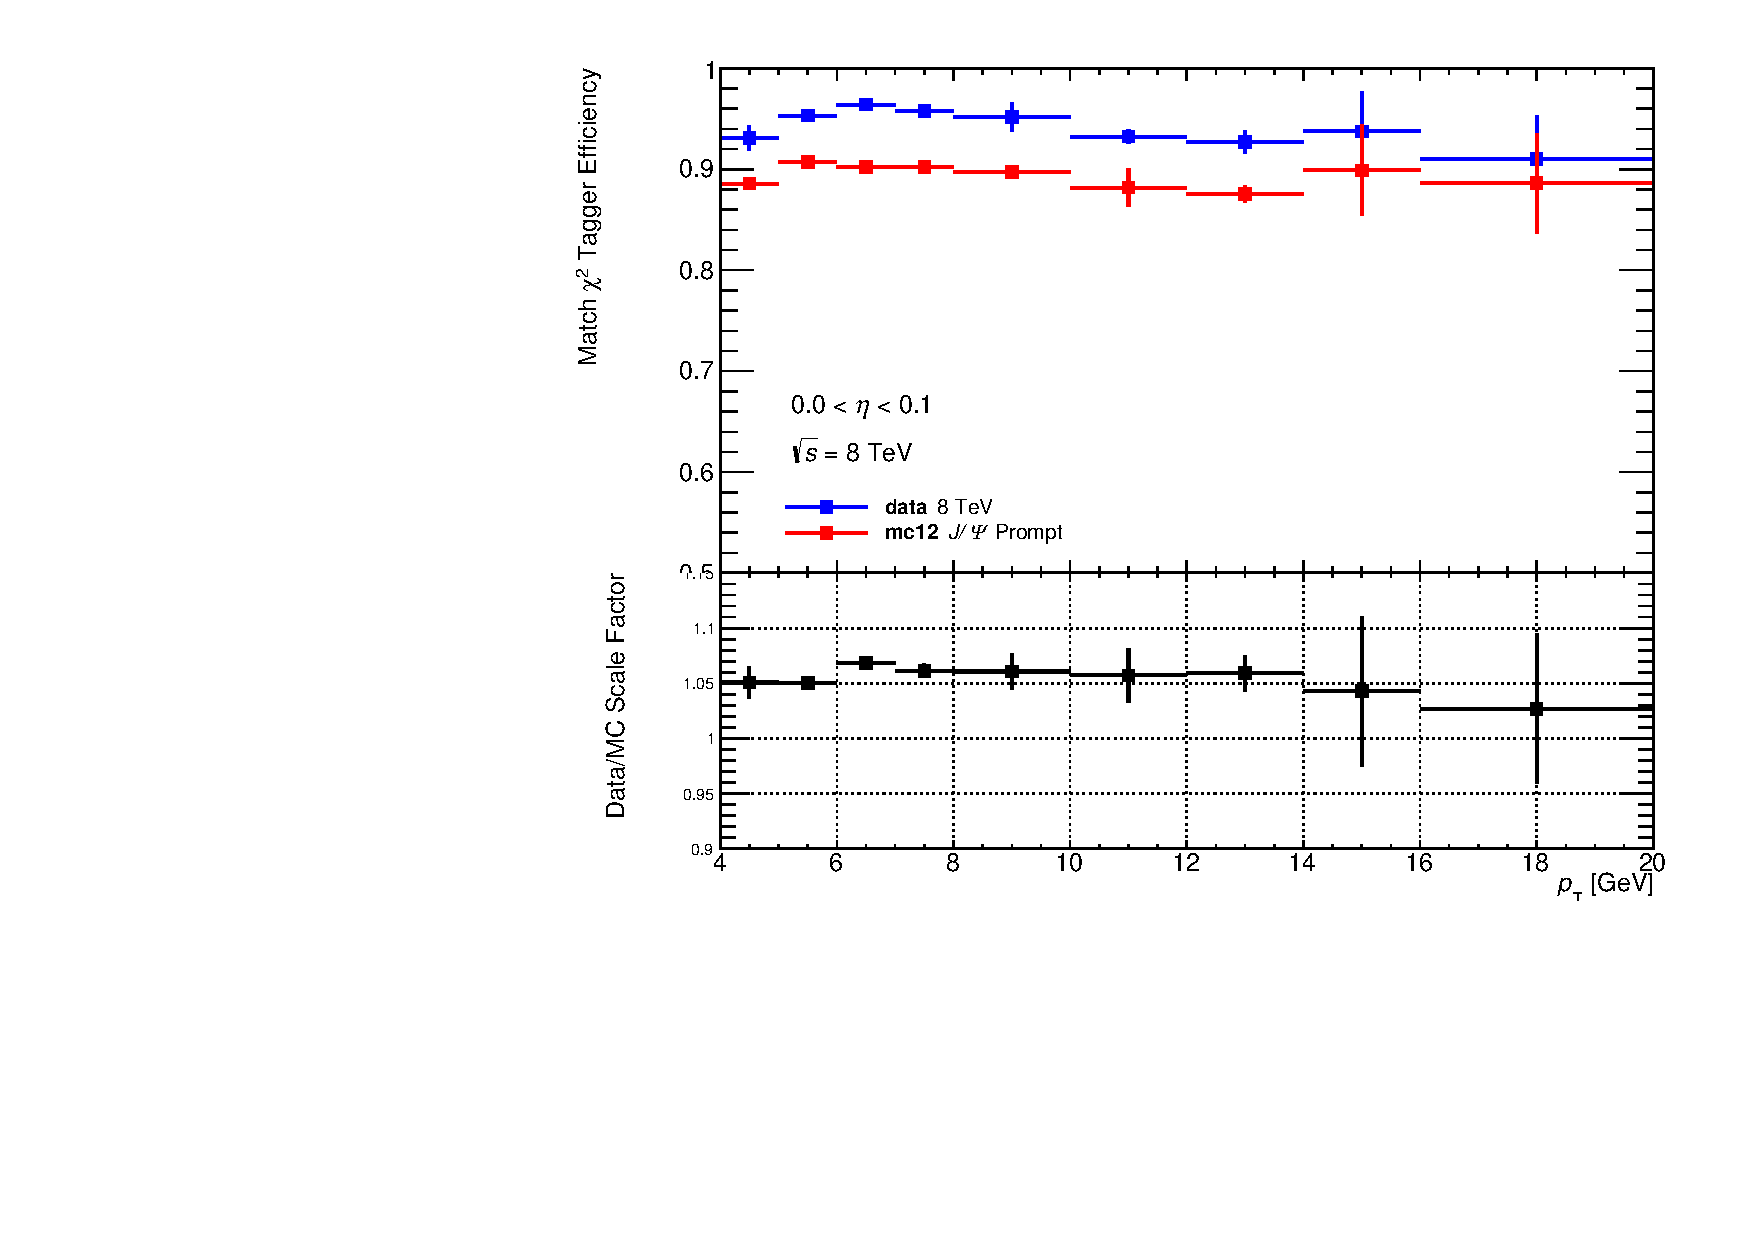
\includegraphics[width=\textwidth]{PartCalibration2012/Plots/SFPlots/Crack_A_smt.pdf}
        \caption{Crack A Region.}\label{fig:CalibrationScaleFactorCrackA}
    \end{subfigure}
  
    \begin{subfigure}[b]{0.85\textwidth}
        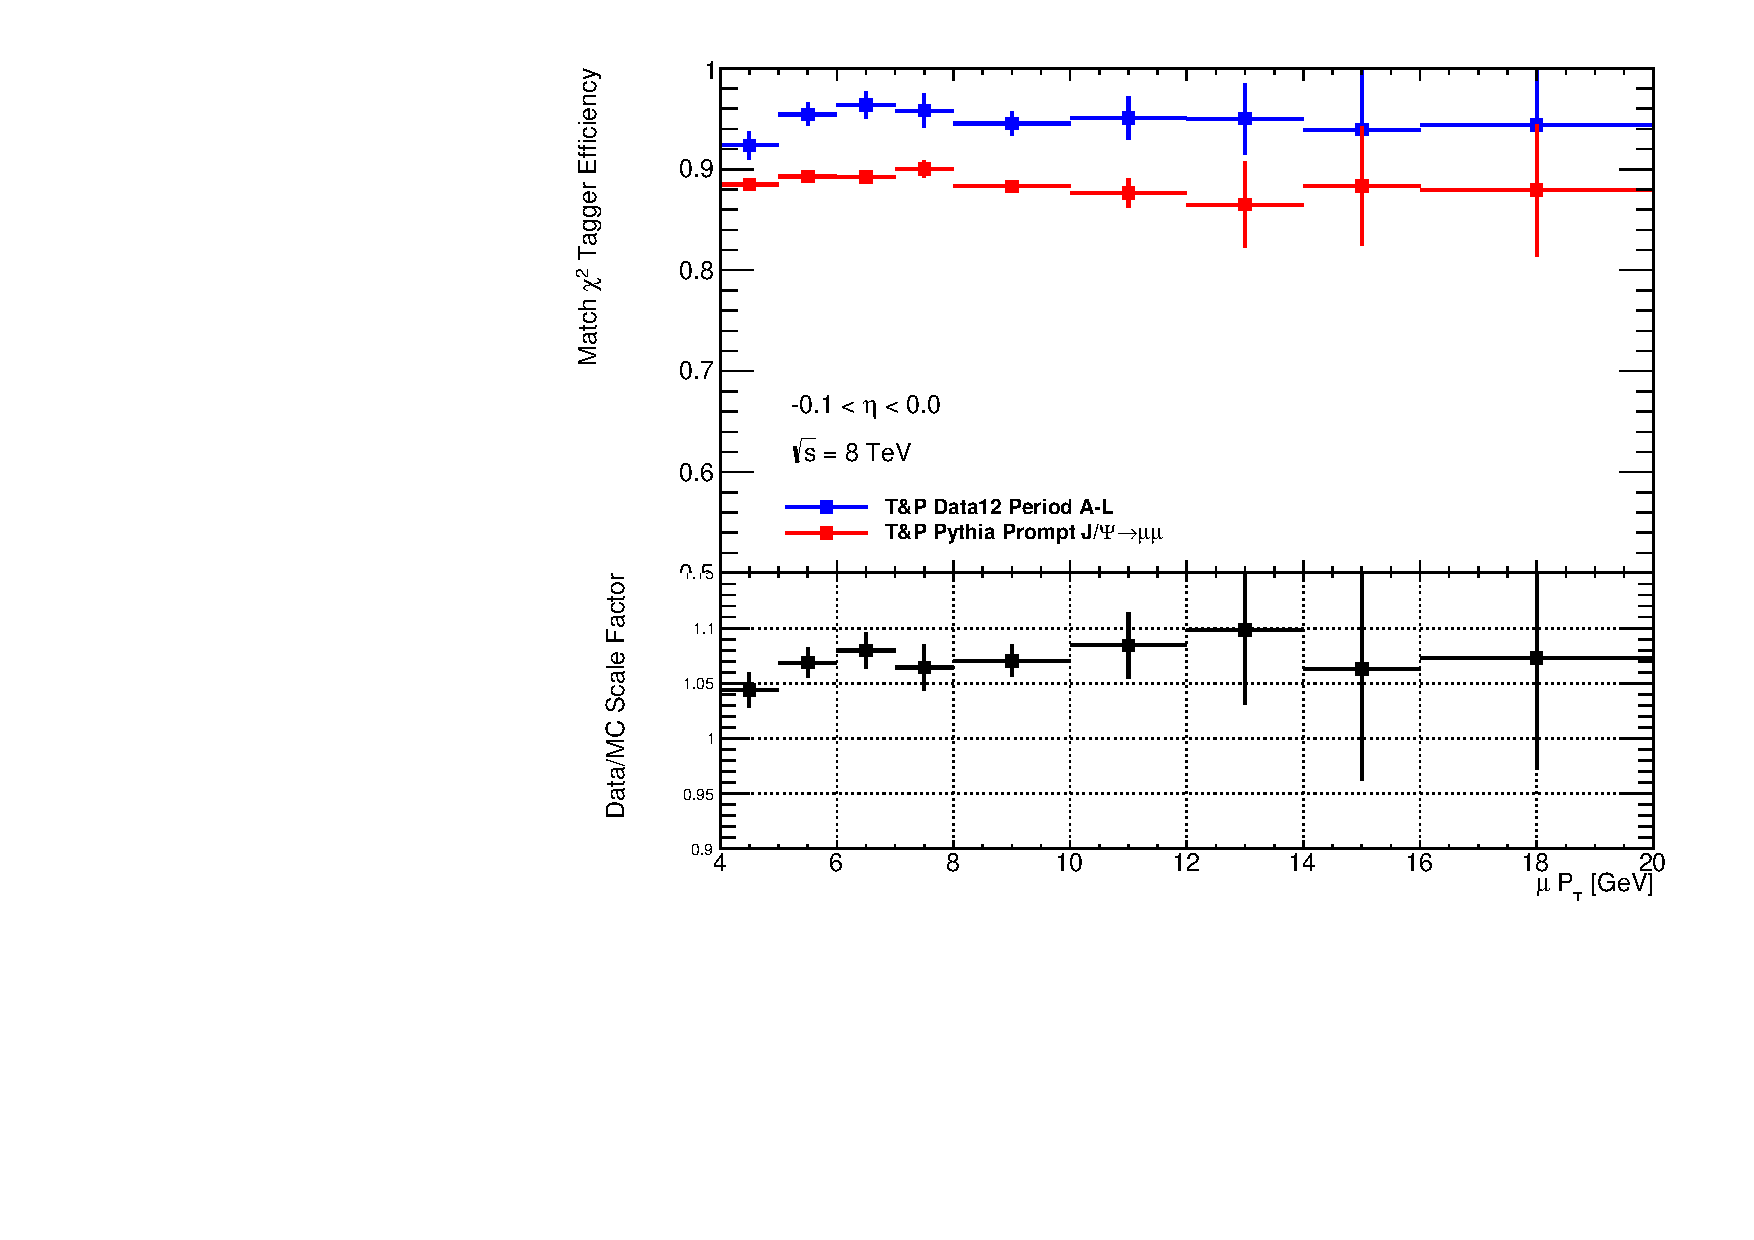
\includegraphics[width=\textwidth]{PartCalibration2012/Plots/SFPlots/Crack_C_smt.pdf}
        \caption{Crack C Region.}\label{fig:CalibrationScaleFactorCrackC}
    \end{subfigure}
    \caption[\xsm\ efficiencies and scale factors in the crack region of the detector for side A and C.]{\xsm\ efficiencies and scale factors in the crack region of the detector for side \subref{fig:CalibrationScaleFactorCrackA} A and \subref{fig:CalibrationScaleFactorCrackC} C.}\label{fig:CalibrationScaleFactorCrack}
\end{figure}

% Barrel Region
\begin{figure}[htbp]
  \centering
    \begin{subfigure}[b]{0.85\textwidth}
        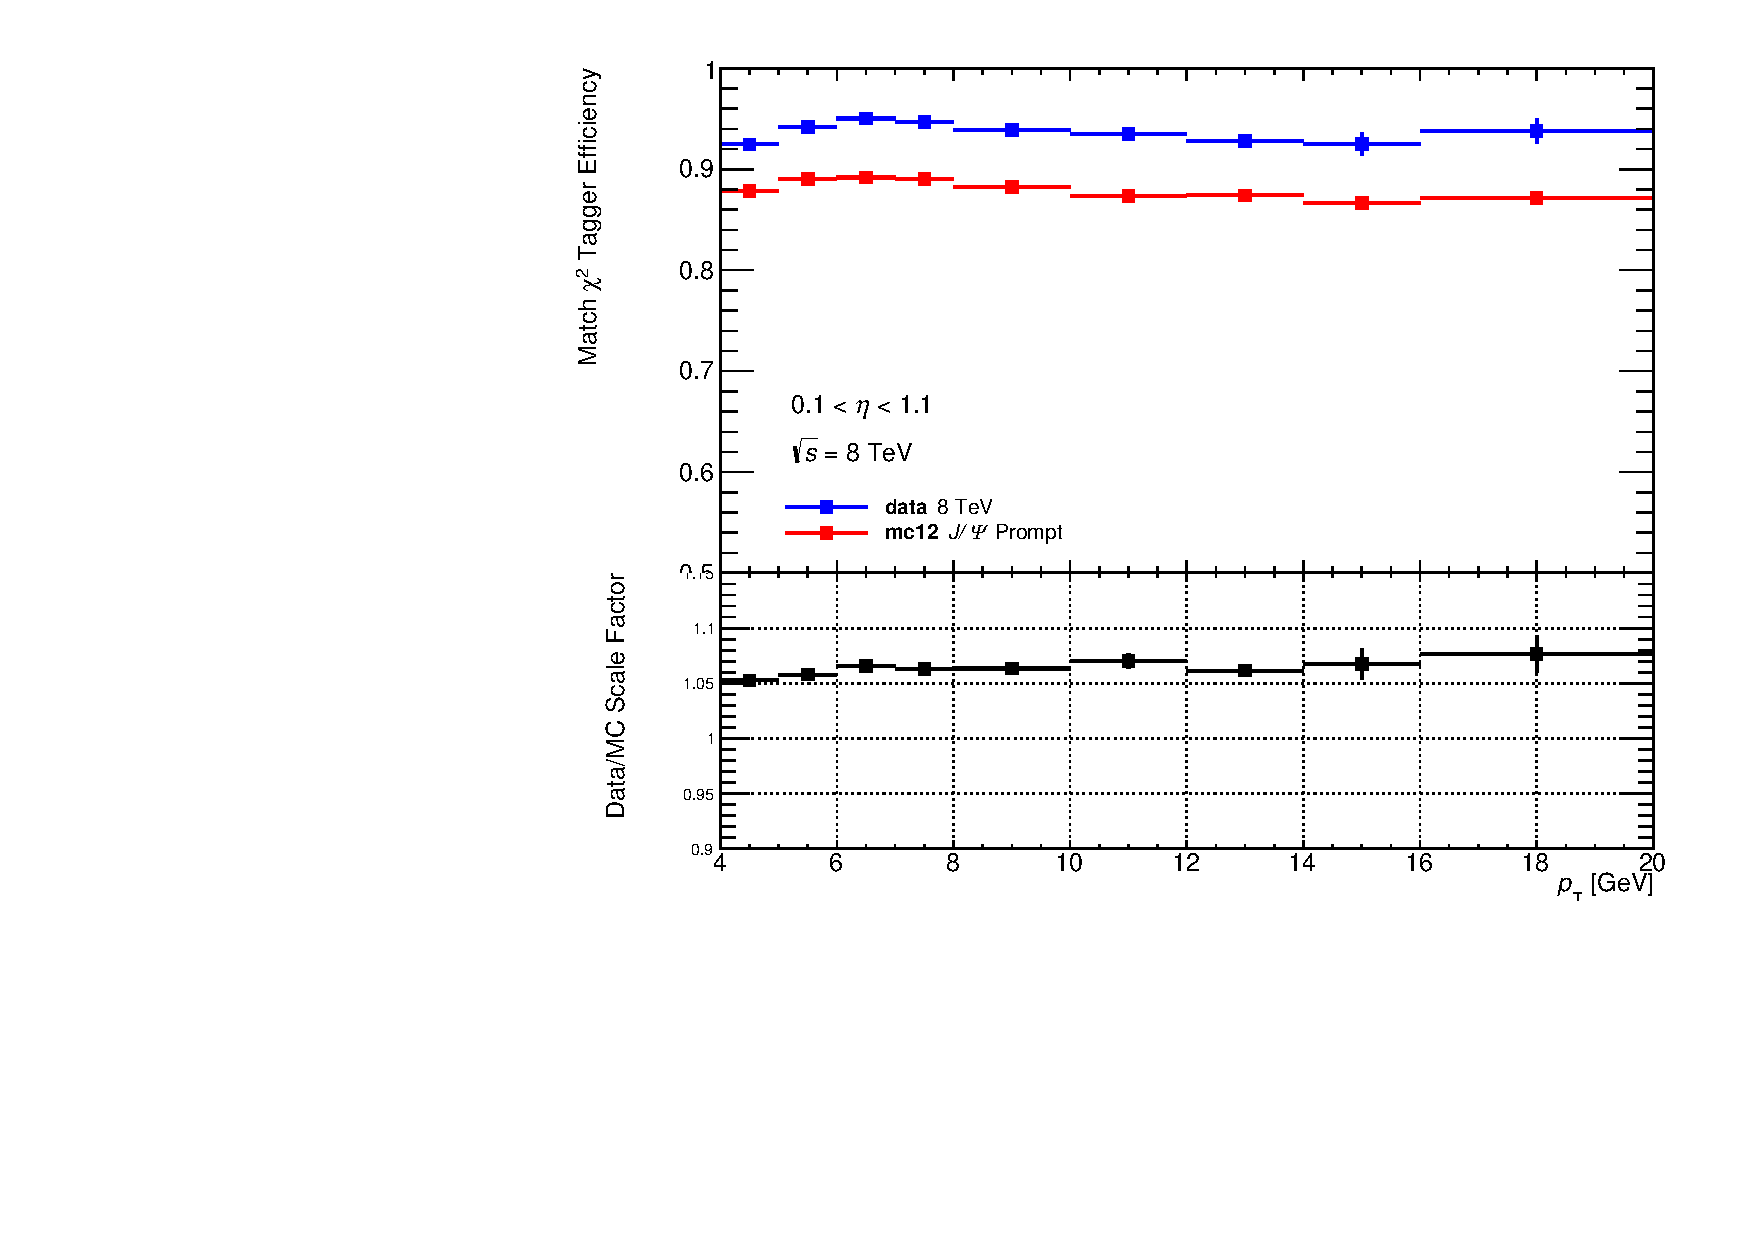
\includegraphics[width=\textwidth]{PartCalibration2012/Plots/SFPlots/Barrel_A_smt.pdf}
        \caption{Barrel A Region.}\label{fig:CalibrationScaleFactorBarrelA}
    \end{subfigure}
    
    \begin{subfigure}[b]{0.85\textwidth}
        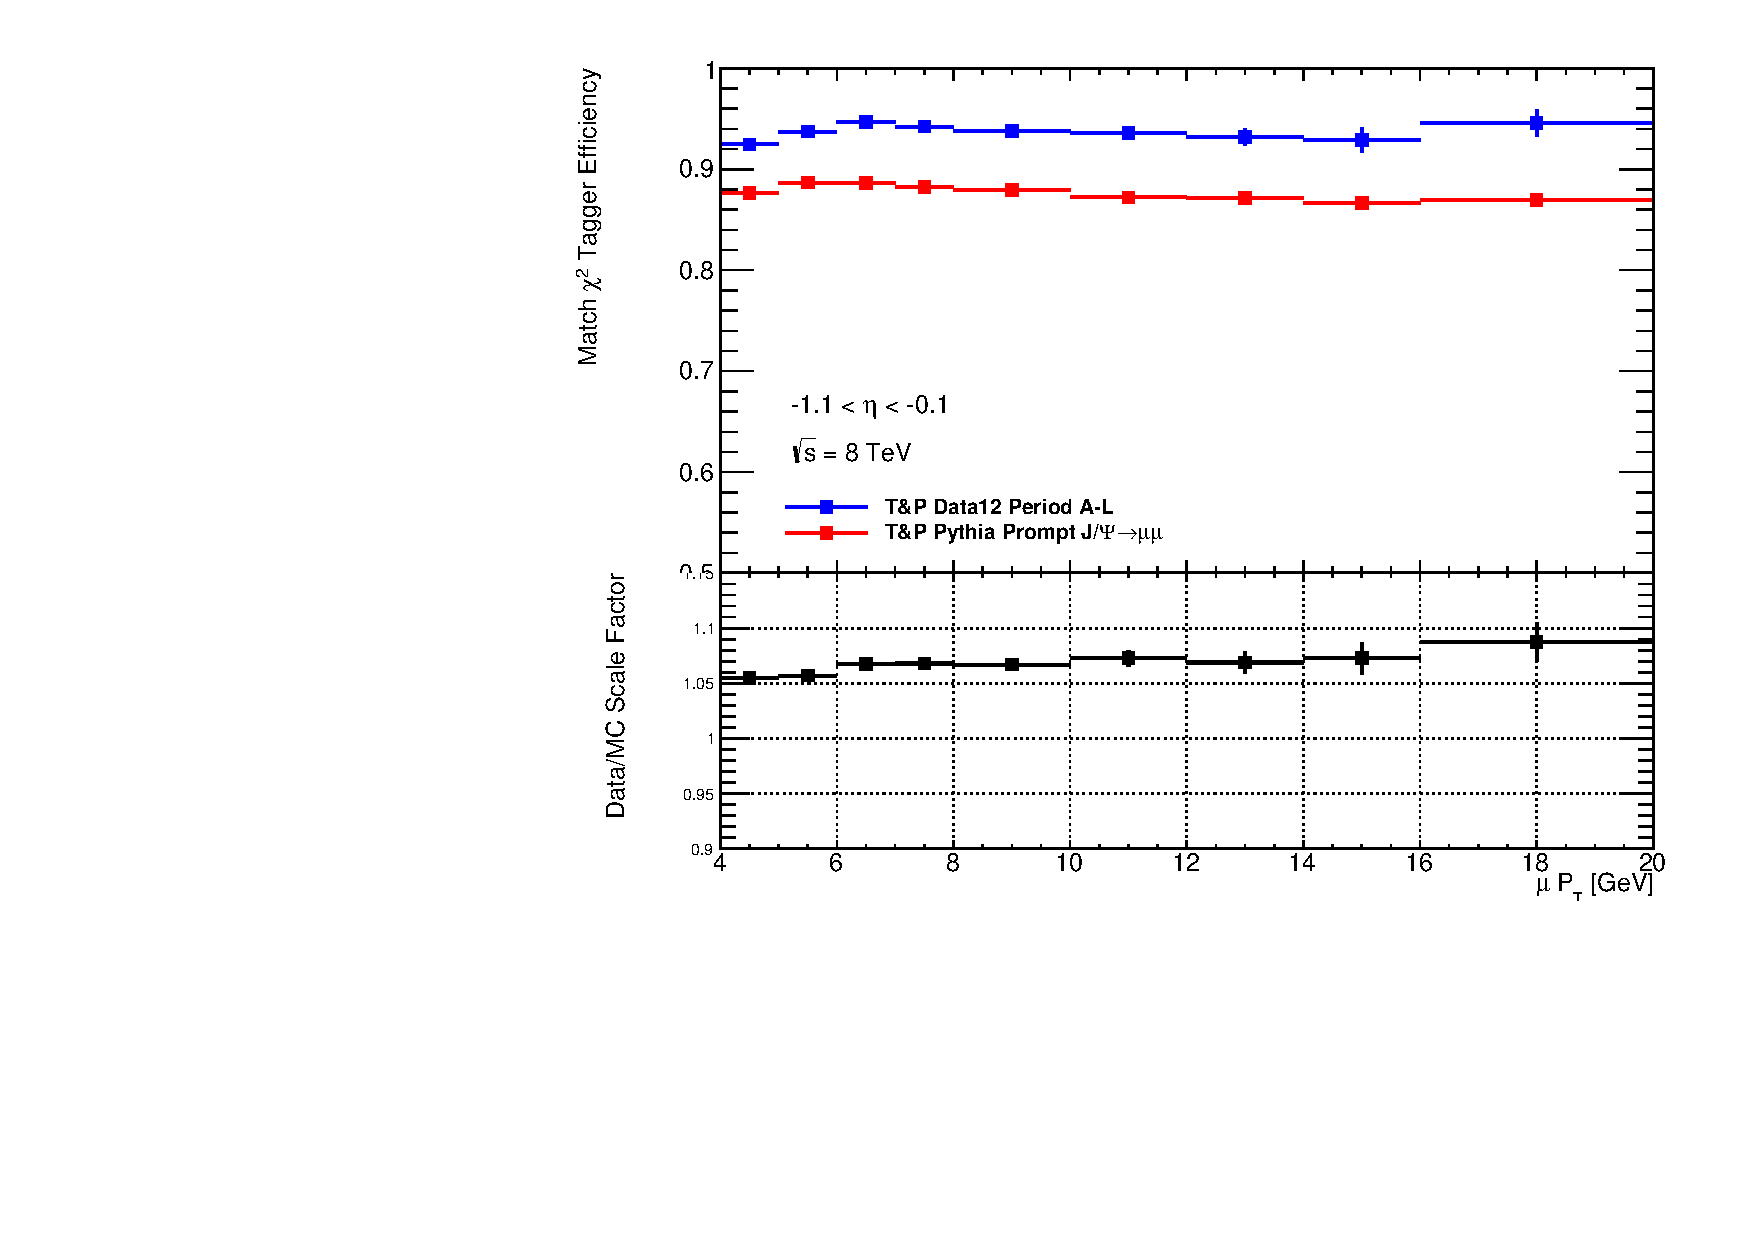
\includegraphics[width=\textwidth]{PartCalibration2012/Plots/SFPlots/Barrel_C_smt.pdf}
        \caption{Barrel C Region.}\label{fig:CalibrationScaleFactorBarrelC}
    \end{subfigure}
    \caption[\xsm\ efficiencies and scale factors in the barrel region of the detector for side A and C.]{\xsm\ efficiencies and scale factors in the barrel region of the detector for side \subref{fig:CalibrationScaleFactorBarrelA} A and \subref{fig:CalibrationScaleFactorBarrelC} C.}\label{fig:CalibrationScaleFactorBarrel}
\end{figure}

% Transition Region
\begin{figure}[htbp]
  \centering
  \begin{subfigure}[b]{0.85\textwidth}
    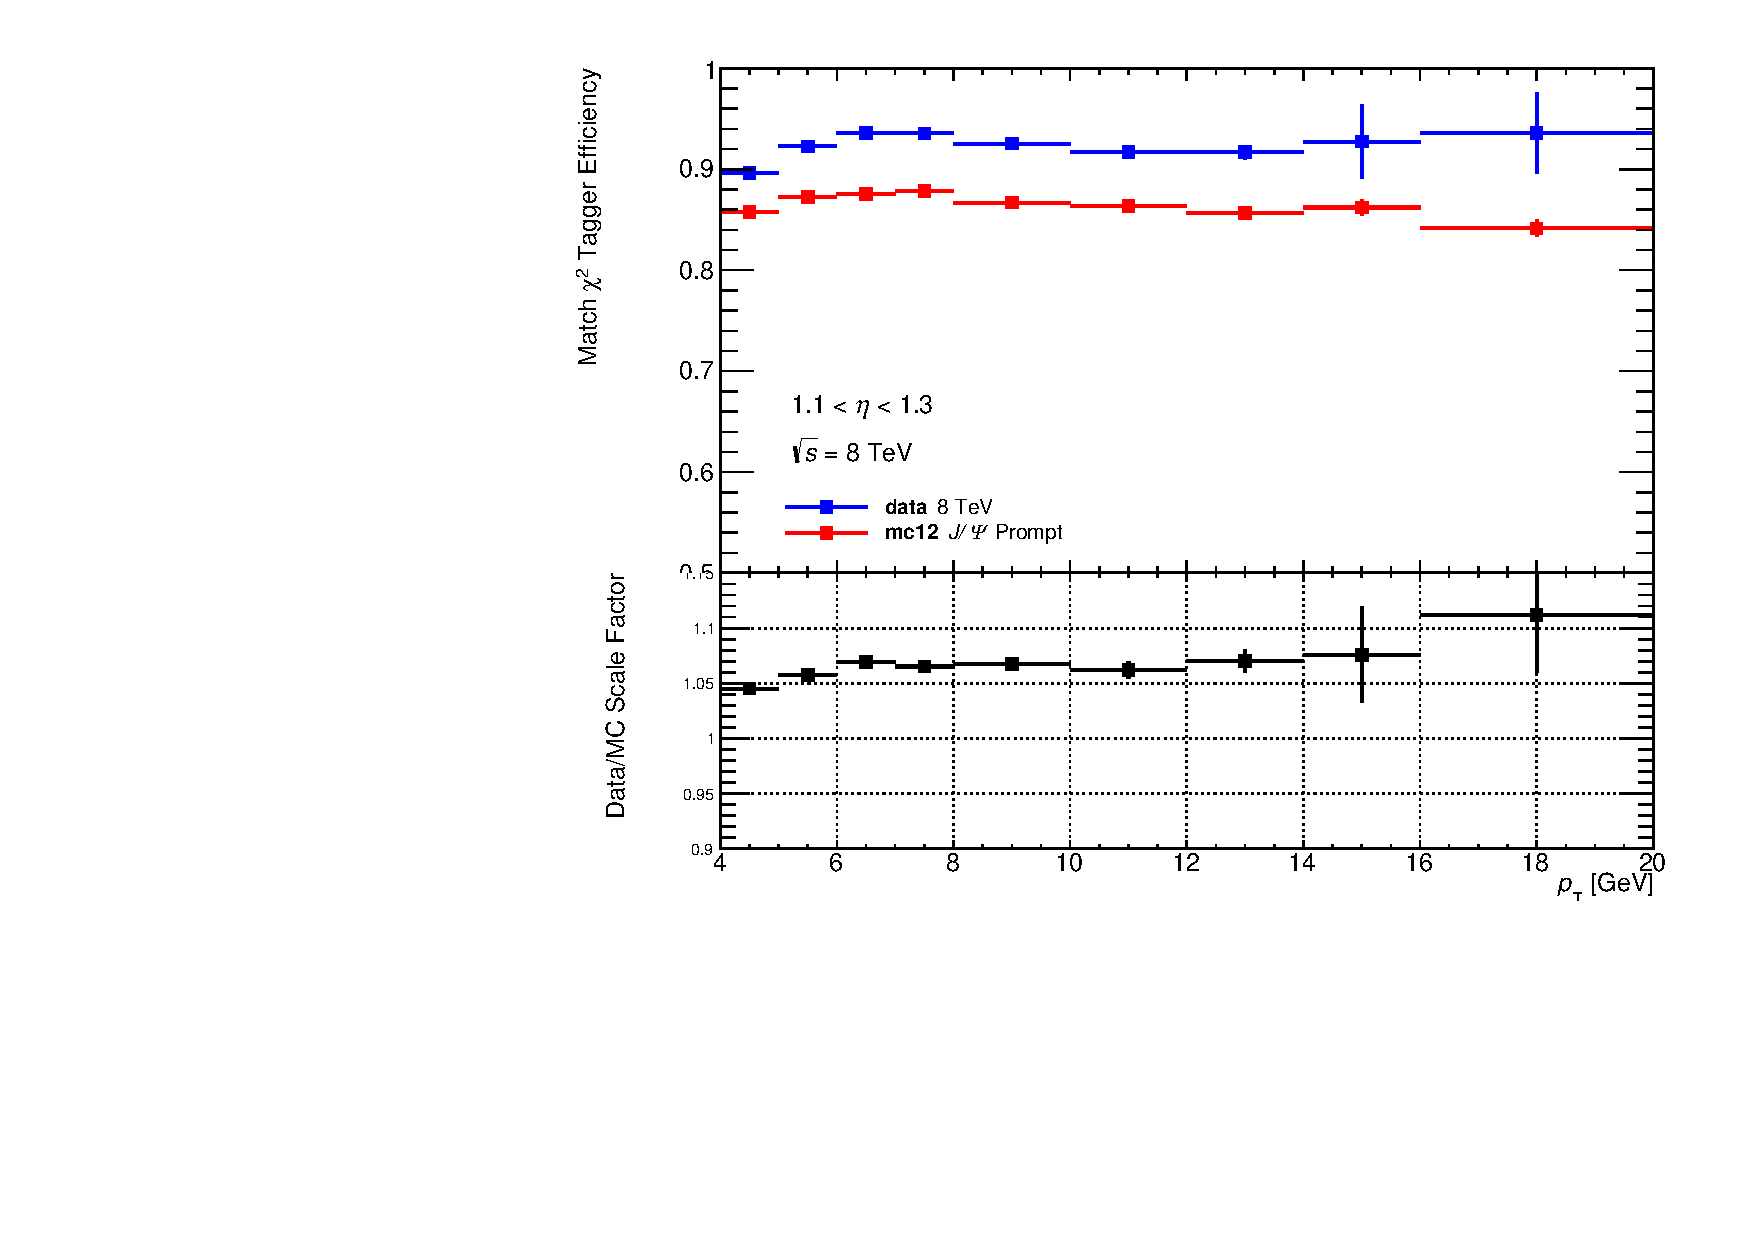
\includegraphics[width=\textwidth]{PartCalibration2012/Plots/SFPlots/Transition_A_smt.pdf}
    \caption{Transition A Region.}\label{fig:CalibrationScaleFactorTransitionA}
  \end{subfigure}
  
  \begin{subfigure}[b]{0.85\textwidth}
    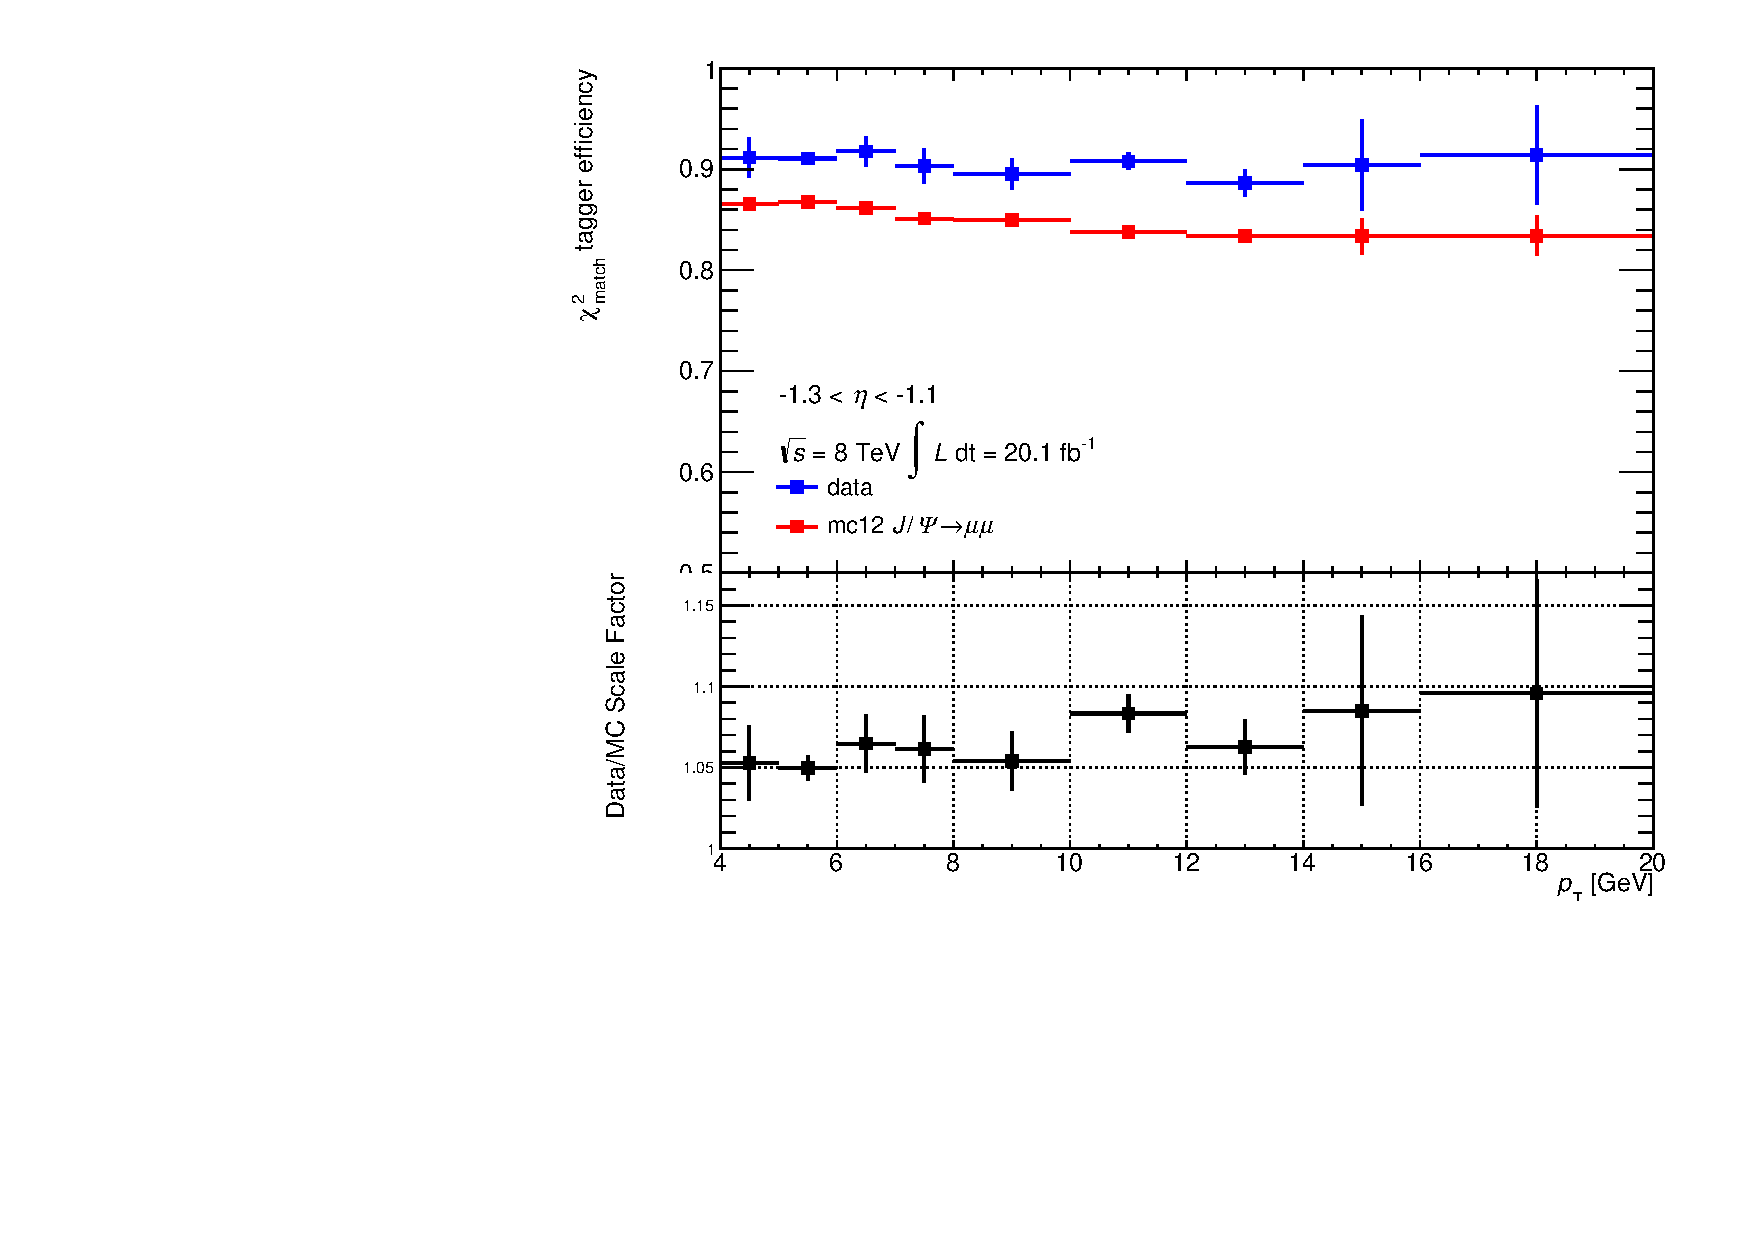
\includegraphics[width=\textwidth]{PartCalibration2012/Plots/SFPlots/Transition_C_smt.pdf}
    \caption{Transition C Region.}\label{fig:CalibrationScaleFactorTransitionC}
  \end{subfigure}
  \caption[\xsm\ efficiencies and scale factors in the transition region of the detector for side A and C.]{\xsm\ efficiencies and scale factors in the transition region of the detector for side \subref{fig:CalibrationScaleFactorTransitionA} A and \subref{fig:CalibrationScaleFactorTransitionC} C.}\label{fig:CalibrationScaleFactorTransition}
\end{figure}

% Endcap Region
\begin{figure}[htbp]
  \centering
  \begin{subfigure}[b]{0.85\textwidth}
    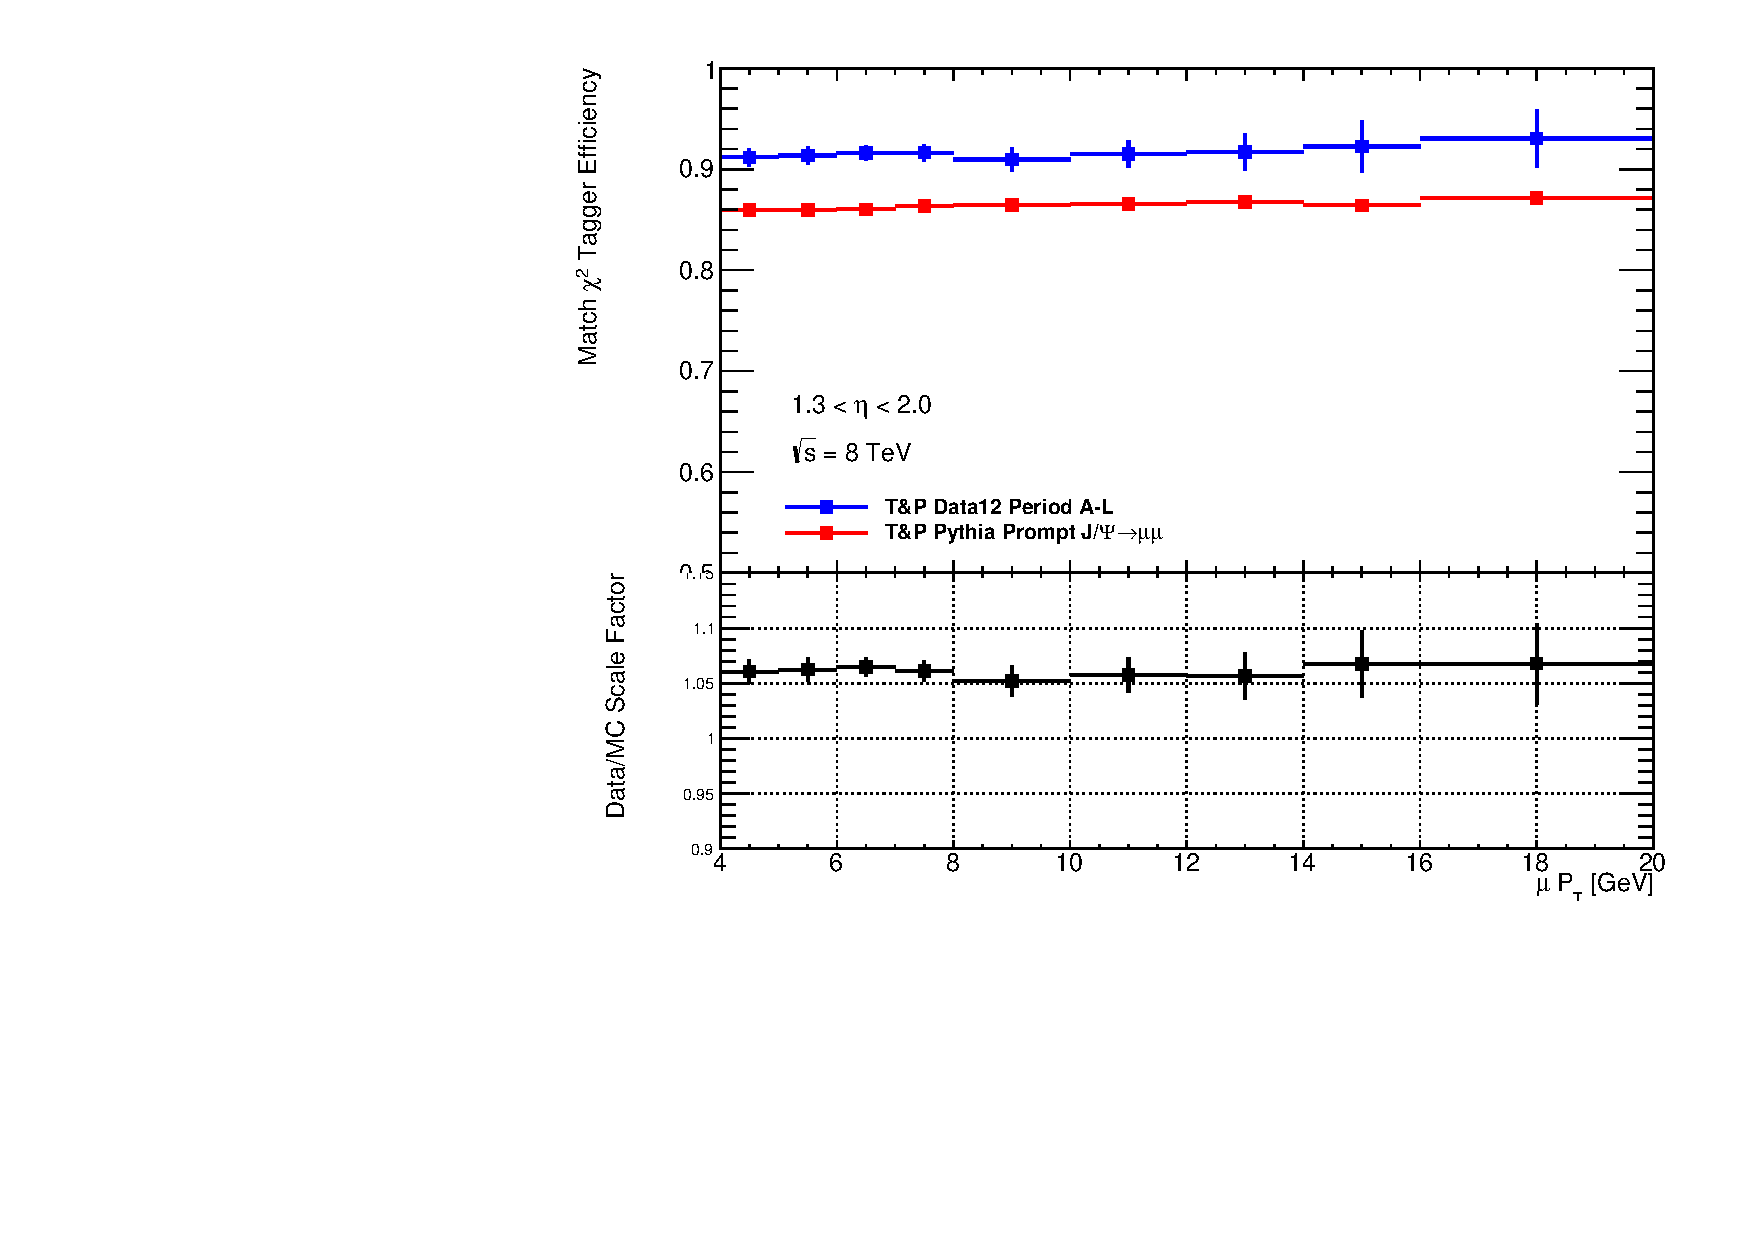
\includegraphics[width=\textwidth]{PartCalibration2012/Plots/SFPlots/Endcap_A_smt.pdf}
    \caption{End-cap A Region.}\label{fig:CalibrationScaleFactorEndcapA}
  \end{subfigure}
  
  \begin{subfigure}[b]{0.85\textwidth}
    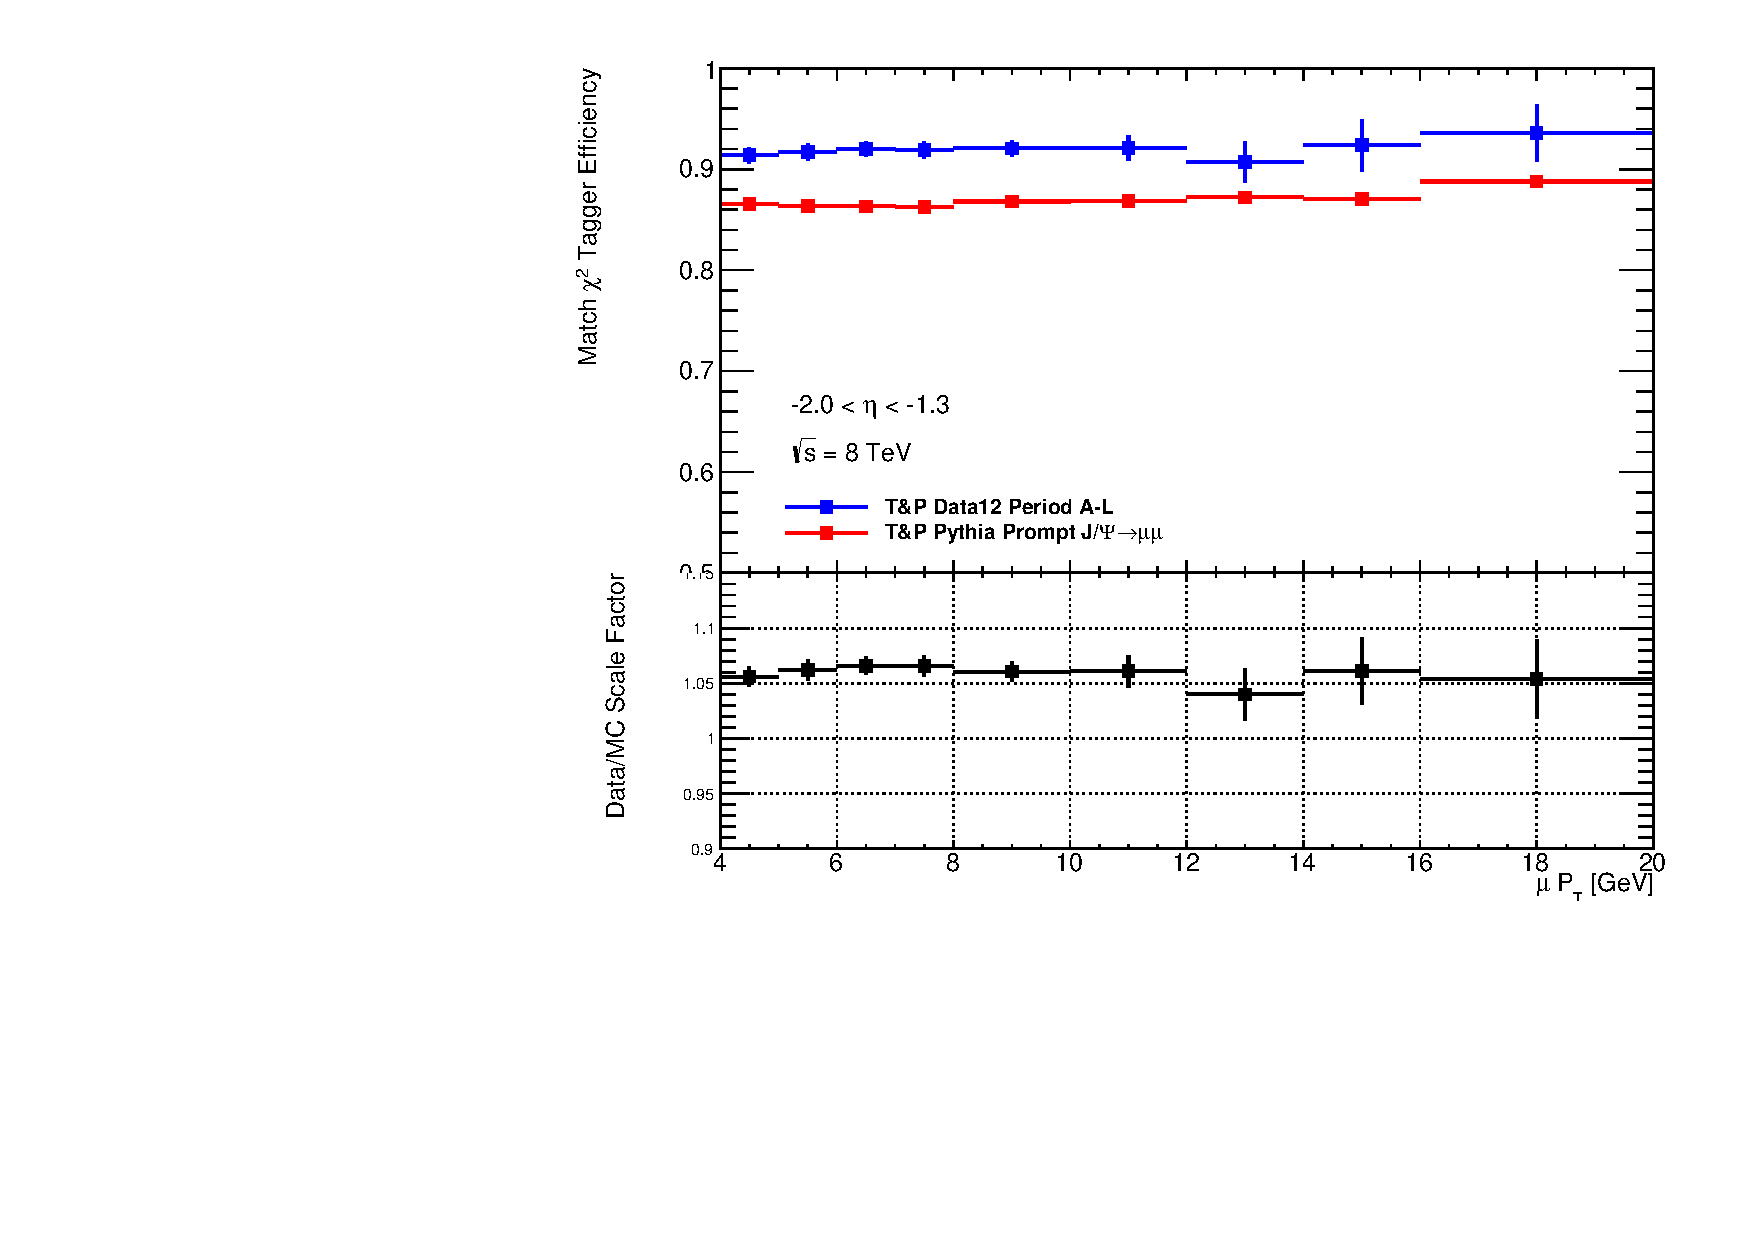
\includegraphics[width=\textwidth]{PartCalibration2012/Plots/SFPlots/Endcap_C_smt.pdf}
    \caption{End-cap C Region.}\label{fig:CalibrationScaleFactorEndcapC}
  \end{subfigure}
  \caption[\xsm\ efficiencies and scale factors in the end-cap region of the detector for side A and C.]{\xsm\ efficiencies and scale factors in the end-cap region of the detector for side \subref{fig:CalibrationScaleFactorEndcapA} A and \subref{fig:CalibrationScaleFactorEndcapC} C.}\label{fig:CalibrationScaleFactorEndcap}
\end{figure}

% Forward Region
\begin{figure}[htbp]
  \centering
  \begin{subfigure}[b]{0.85\textwidth}
    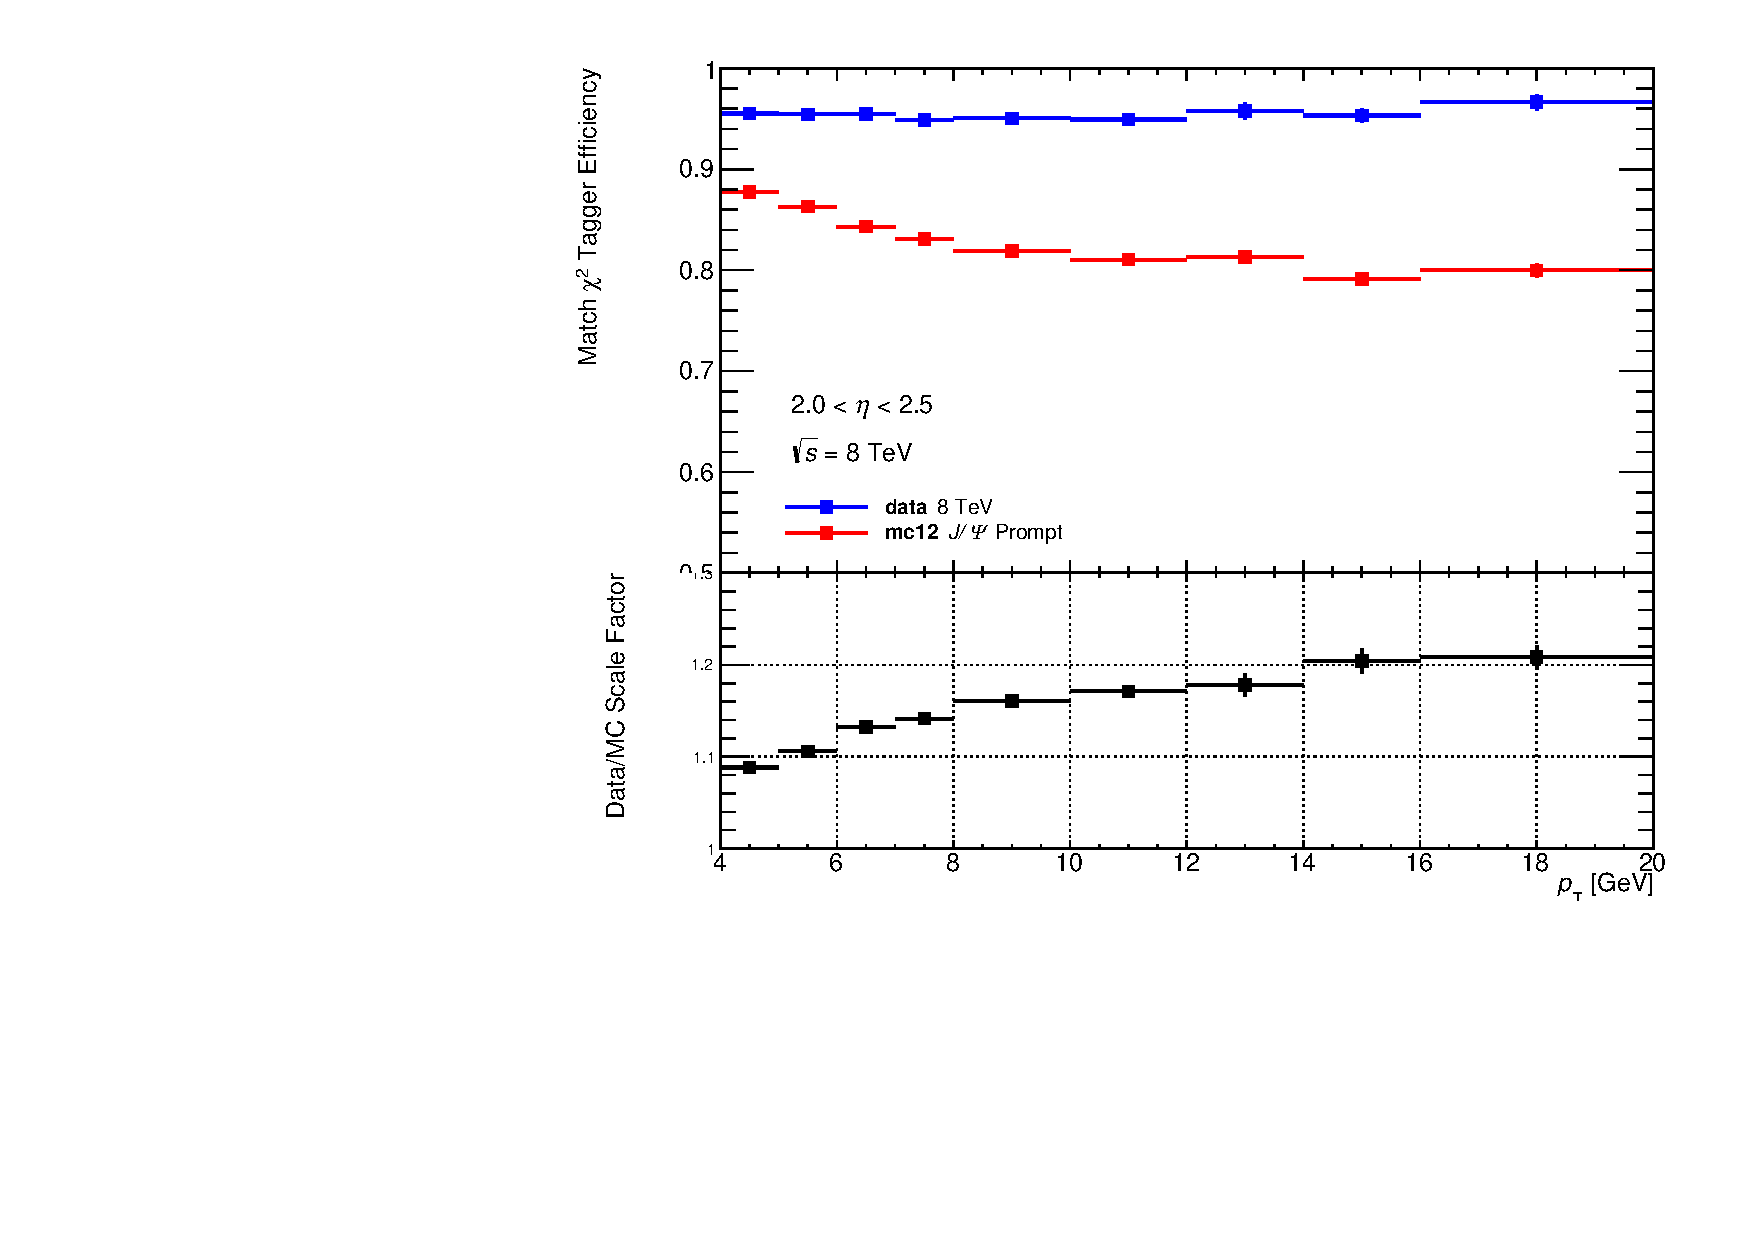
\includegraphics[width=\textwidth]{PartCalibration2012/Plots/SFPlots/Forward_A_smt.pdf}
    \caption{Forward A Region.}\label{fig:CalibrationScaleFactorForwardA}
  \end{subfigure}
  
  \begin{subfigure}[b]{0.85\textwidth}
    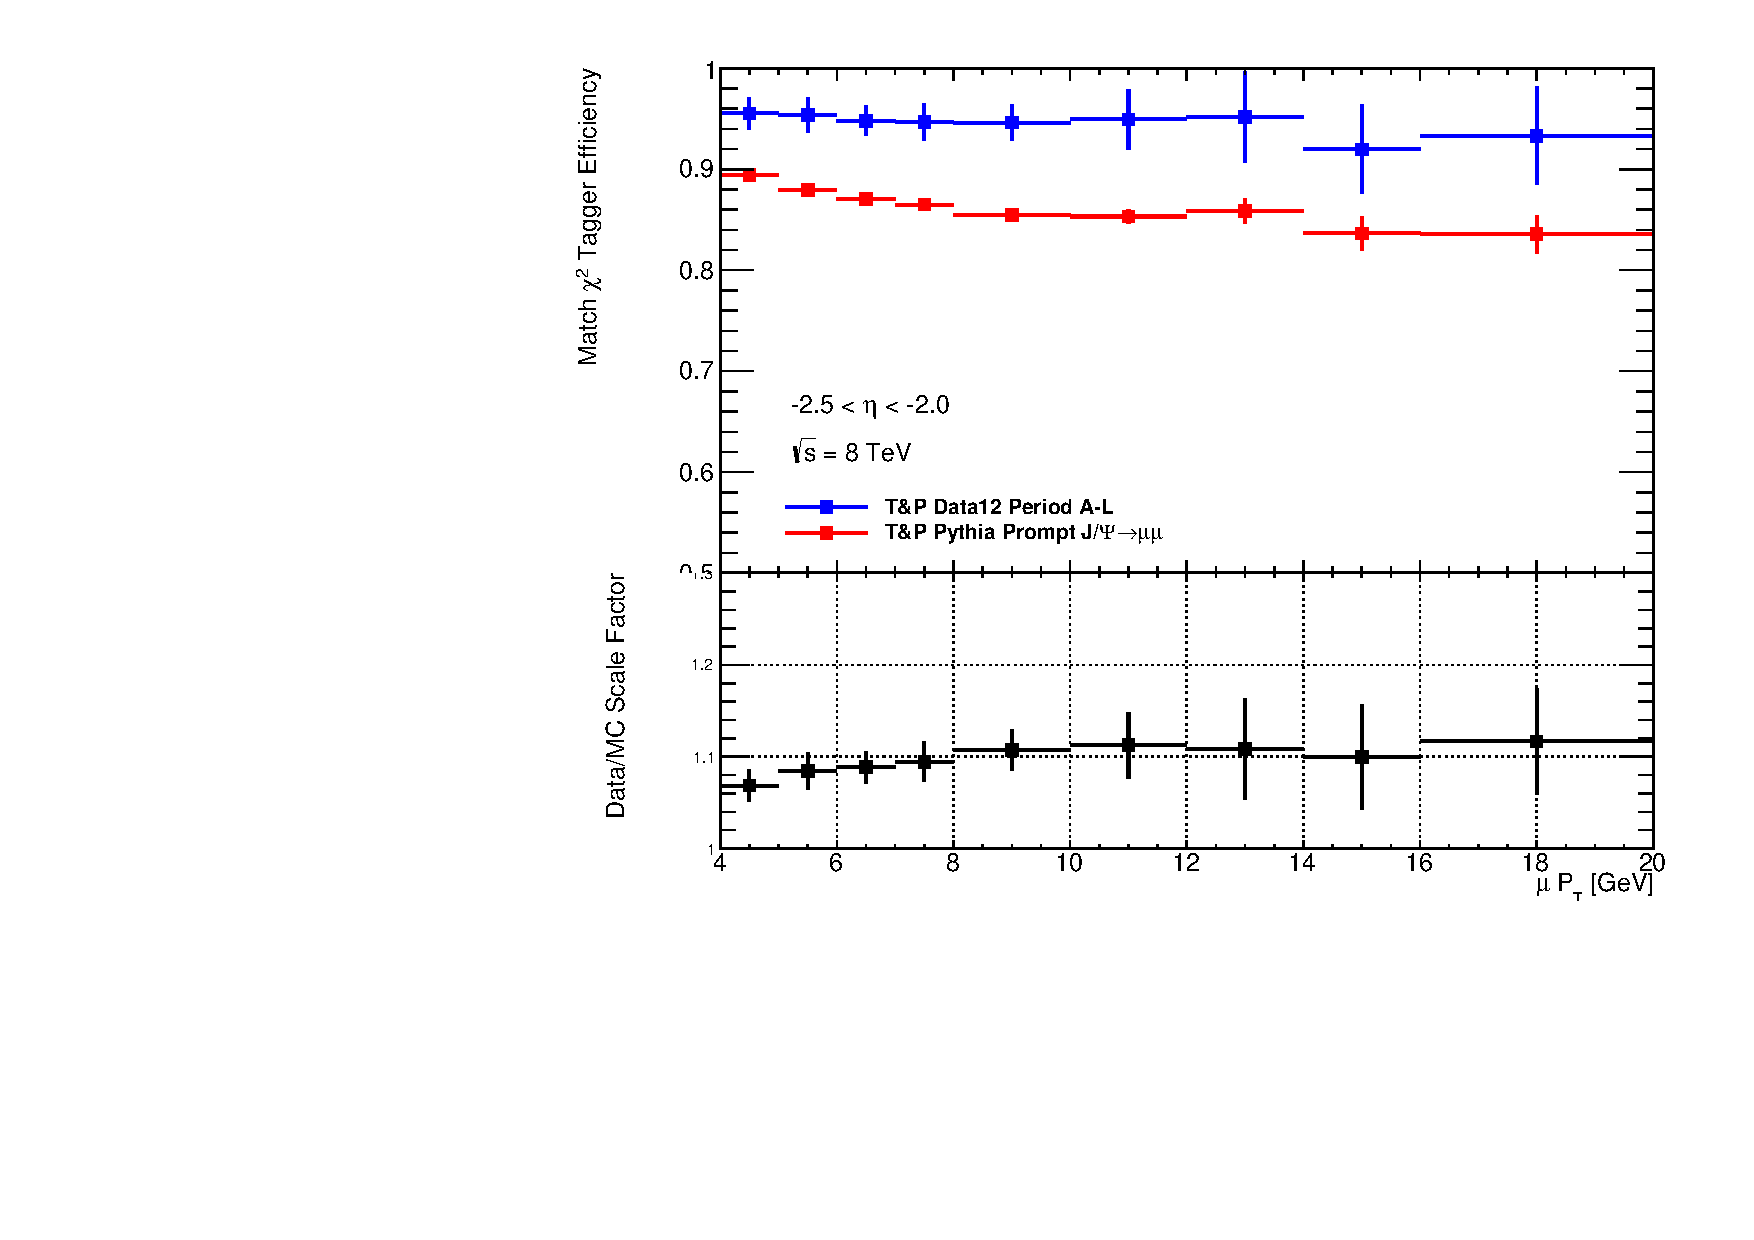
\includegraphics[width=\textwidth]{PartCalibration2012/Plots/SFPlots/Forward_C_smt.pdf}
    \caption{Forward C Region.}\label{fig:CalibrationScaleFactorForwardC}
  \end{subfigure}
  \caption[\xsm\ efficiencies and scale factors in the forward region of the detector for side A and C.]{\xsm\ efficiencies and scale factors in the forward region of the detector for side \subref{fig:CalibrationScaleFactorForwardA} A and \subref{fig:CalibrationScaleFactorForwardC} C.}\label{fig:CalibrationScaleFactorForward}
\end{figure}

% Table of 2012 SF
\begin{table}[htbp]
  \centering
  \tabcolsep=0.11cm
  \ra{1.3}
  \begin{tabular}{@{}%
                    l%
                    *{5}{S[table-format=1.3(3)]}%
                  @{}}
  \toprule
  \pt\ range [\si{\GeV}]   & \multicolumn{5}{c}{Scale Factor in} \\
  \midrule
  \textbf{Side A}          & {Crack}   & {Barrel}  & {Transition} & {End-cap}  & {Forward} \\
  \tabin\numrange{4}{5}   & 1.051(14) & 1.053(1)  & 1.045(5)     & 1.059(2)  & 1.088(2)  \\
  \tabin\numrange{5}{6}   & 1.051(5)  & 1.058(1)  & 1.057(5)     & 1.062(10) & 1.106(3)  \\
  \tabin\numrange{6}{7}   & 1.068(6)  & 1.066(1)  & 1.069(4)     & 1.066(2)  & 1.132(3)  \\
  \tabin\numrange{7}{8}   & 1.061(6)  & 1.063(1)  & 1.065(4)     & 1.062(2)  & 1.142(3)  \\
  \tabin\numrange{8}{10}  & 1.061(16) & 1.063(1)  & 1.068(4)     & 1.063(2)  & 1.161(3)  \\
  \tabin\numrange{10}{12} & 1.057(24) & 1.071(6)  & 1.062(7)     & 1.060(15) & 1.171(6)  \\
  \tabin\numrange{12}{14} & 1.059(16) & 1.062(3)  & 1.070(10)    & 1.057(20) & 1.178(12) \\
  \tabin\numrange{14}{16} & 1.043(68) & 1.069(13) & 1.076(43)    & 1.069(6)  & 1.204(13) \\
  \tabin\numrange{16}{20} & 1.027(77) & 1.077(6)  & 1.112(19)    & 1.067(4)  & 1.208(9)  \\
  \midrule
  \textbf{Side C}          & {Crack}   & {Barrel}  & {Transition} & {End-cap}  & {Forward} \\ 
  \tabin\numrange{4}{5}   & 1.044(14) & 1.055(1)  & 1.053(4)     & 1.056(2)  & 1.064(5)  \\
  \tabin\numrange{5}{6}   & 1.069(5)  & 1.057(1)  & 1.050(15)    & 1.061(8)  & 1.083(3)  \\
  \tabin\numrange{6}{7}   & 1.080(5)  & 1.068(4)  & 1.065(4)     & 1.065(2)  & 1.095(3)  \\
  \tabin\numrange{7}{8}   & 1.064(17) & 1.068(5)  & 1.061(5)     & 1.066(2)  & 1.100(4)  \\
  \tabin\numrange{8}{10}  & 1.070(7)  & 1.067(4)  & 1.054(5)     & 1.061(2)  & 1.101(3)  \\
  \tabin\numrange{10}{12} & 1.089(10) & 1.073(3)  & 1.083(22)    & 1.062(3)  & 1.107(6)  \\
  \tabin\numrange{12}{14} & 1.095(15) & 1.069(9)  & 1.063(28)    & 1.049(5)  & 1.114(8)  \\
  \tabin\numrange{14}{16} & 1.059(32) & 1.076(6)  & 1.085(14)    & 1.061(6)  & 1.107(13) \\
  \tabin\numrange{16}{20} & 1.109(32) & 1.088(3)  & 1.096(21)    & 1.050(4)  & 1.120(9)  \\
  \bottomrule
  \end{tabular}
  \caption[Data/MC Scale Factors for 2012 Data in all five regions of the detector as a function of \pt.]{Data/MC Scale Factors for 2012 Data in all five regions of the detector as a function of \pt. The uncertainties include systematic and statistical components as described in Section~\ref{sec:CalibrationUncertainty}.}\label{tab:Calibration2012SF}
\end{table}

\subsubsection{Isolation dependence}\label{sec:CalibrationEfficienciesIsolation}

The muons from the $\textrm{J}/\psi\textrm{s}$ used in this calibration are produced in isolation, meaning there is very little energetic activity surrounding them in the detector. In contrast, muons from semileptonic decay of $b$-quarks in \ttbar\ events are produced amongst the tracks associated with the $b$-jet.

For the results of the calibration on \jpsi\ to be applicable, the performance of the \xsm\ tagger must not affected by the isolation of the muon. In this calibration, the nine isolation variables defined in Section~\ref{sec:DetectorElReco} are considered.

The isolated nature of muons in \jpsi\ events limits the number of muons available at higher isolation values. This is more significant in simulation compared to the collision data which contains non-isolated muons. There appears to be no dependence on any of the isolation variables examined (Figures~\ref{fig:CalibrationIsoEtcone},~\ref{fig:CalibrationIsoPtcone} and~\ref{fig:CalibrationIsoNucone}).

% etcone
\begin{figure}[htbp]
  \centering
    \begin{subfigure}[b]{0.76\textwidth}
      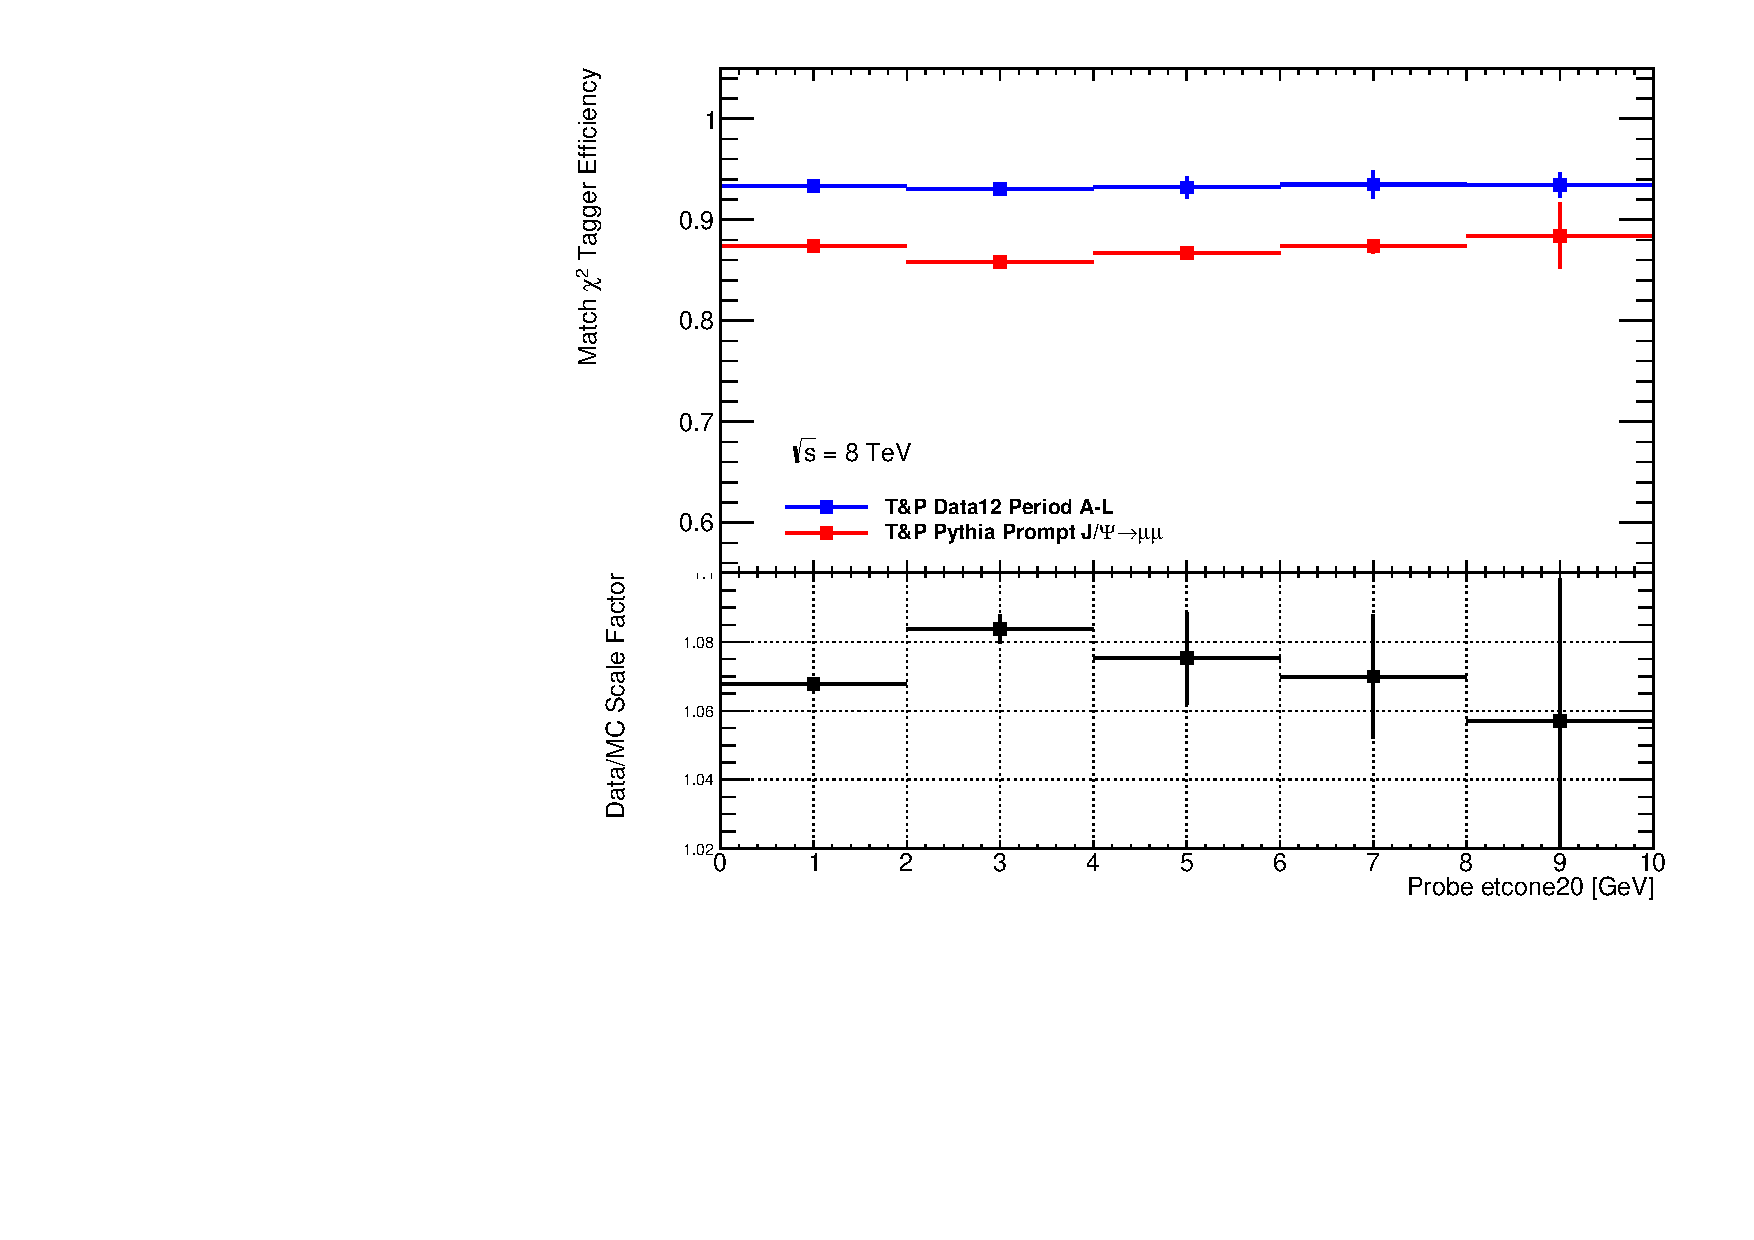
\includegraphics[width=\textwidth]{PartCalibration2012/Plots/SFPlots/etcone20_smt.pdf}
      \caption{$\sum \Et$ in cone $\Delta R=0.2$}\label{fig:CalibrationIsoEtcone20}
    \end{subfigure}
    
    \begin{subfigure}[b]{0.76\textwidth}
      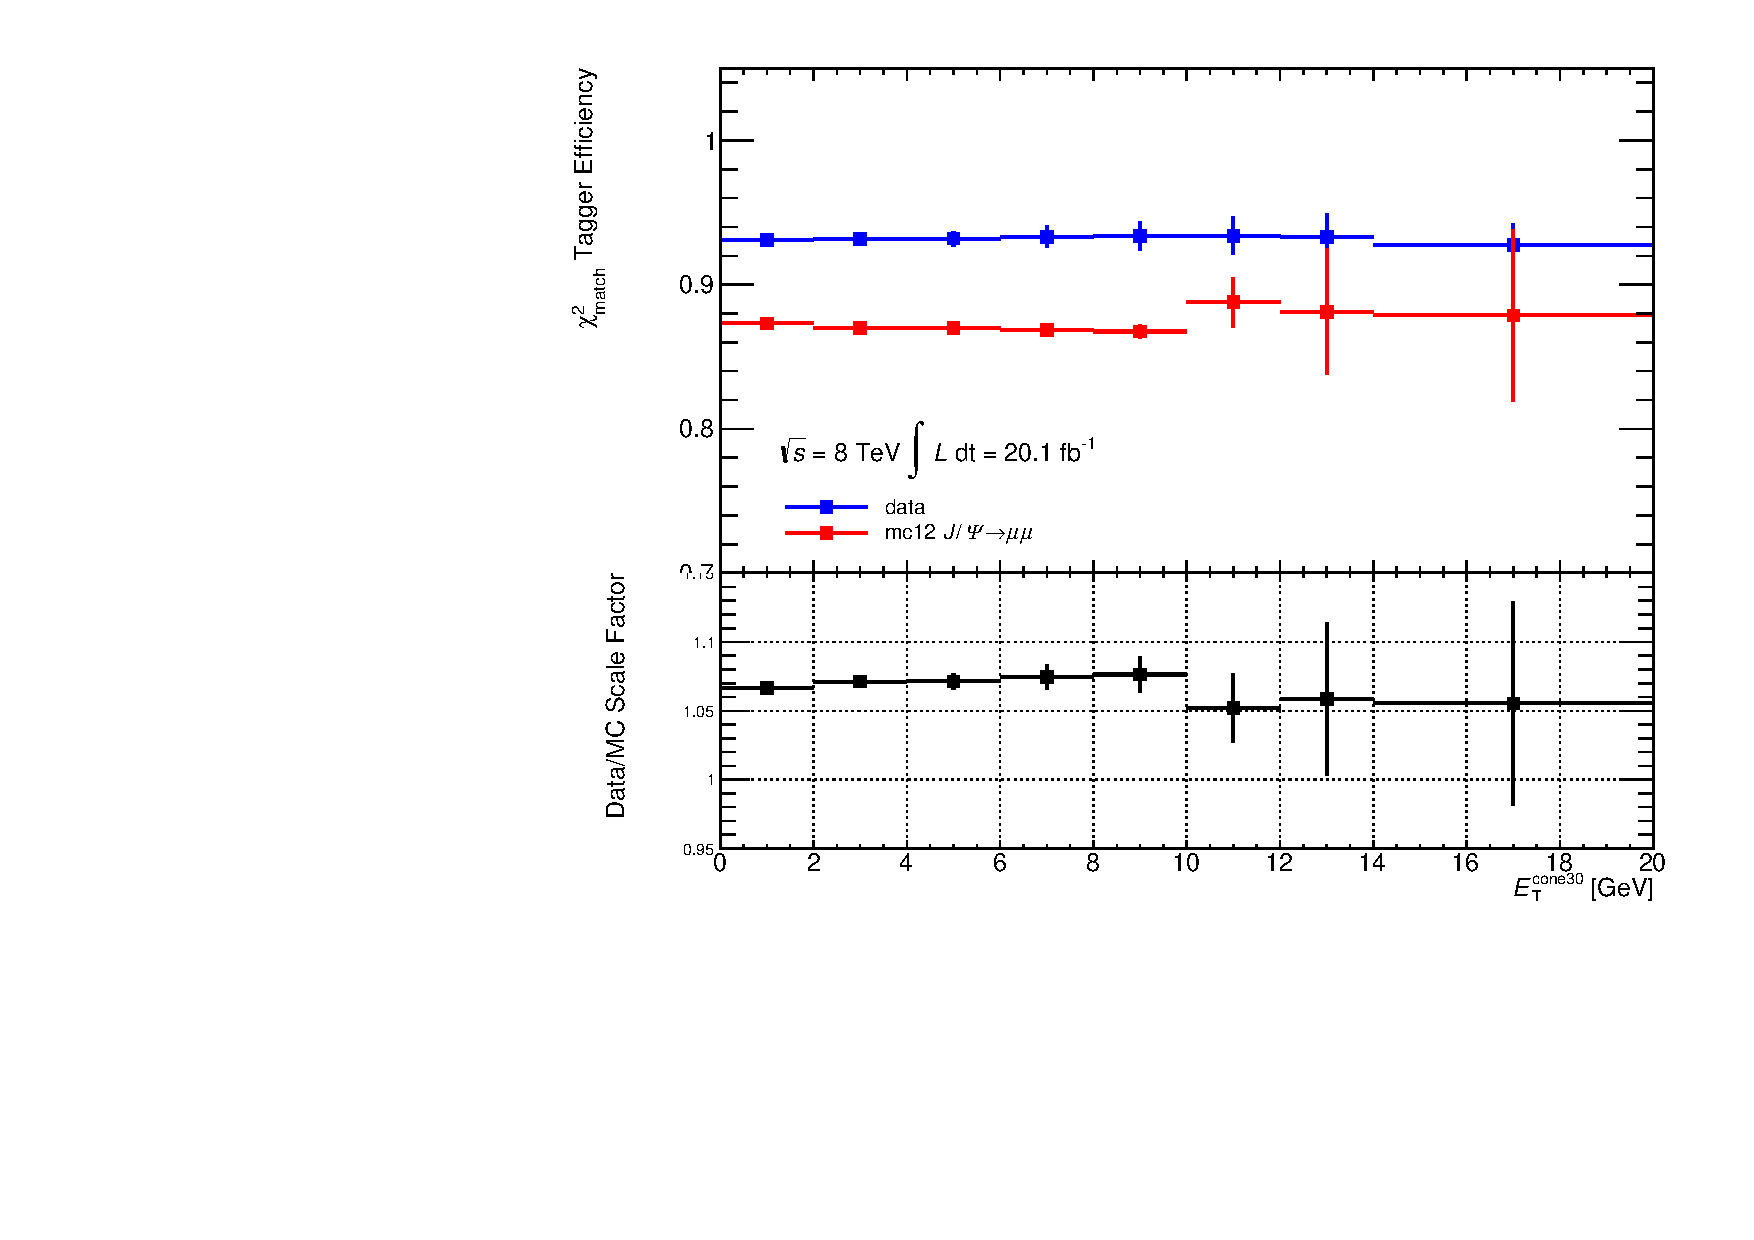
\includegraphics[width=\textwidth]{PartCalibration2012/Plots/SFPlots/etcone30_smt.pdf}
      \caption{$\sum \Et$ in cone $\Delta R=0.3$}\label{fig:CalibrationIsoEtcone30}
    \end{subfigure}

    \begin{subfigure}[b]{0.76\textwidth}
      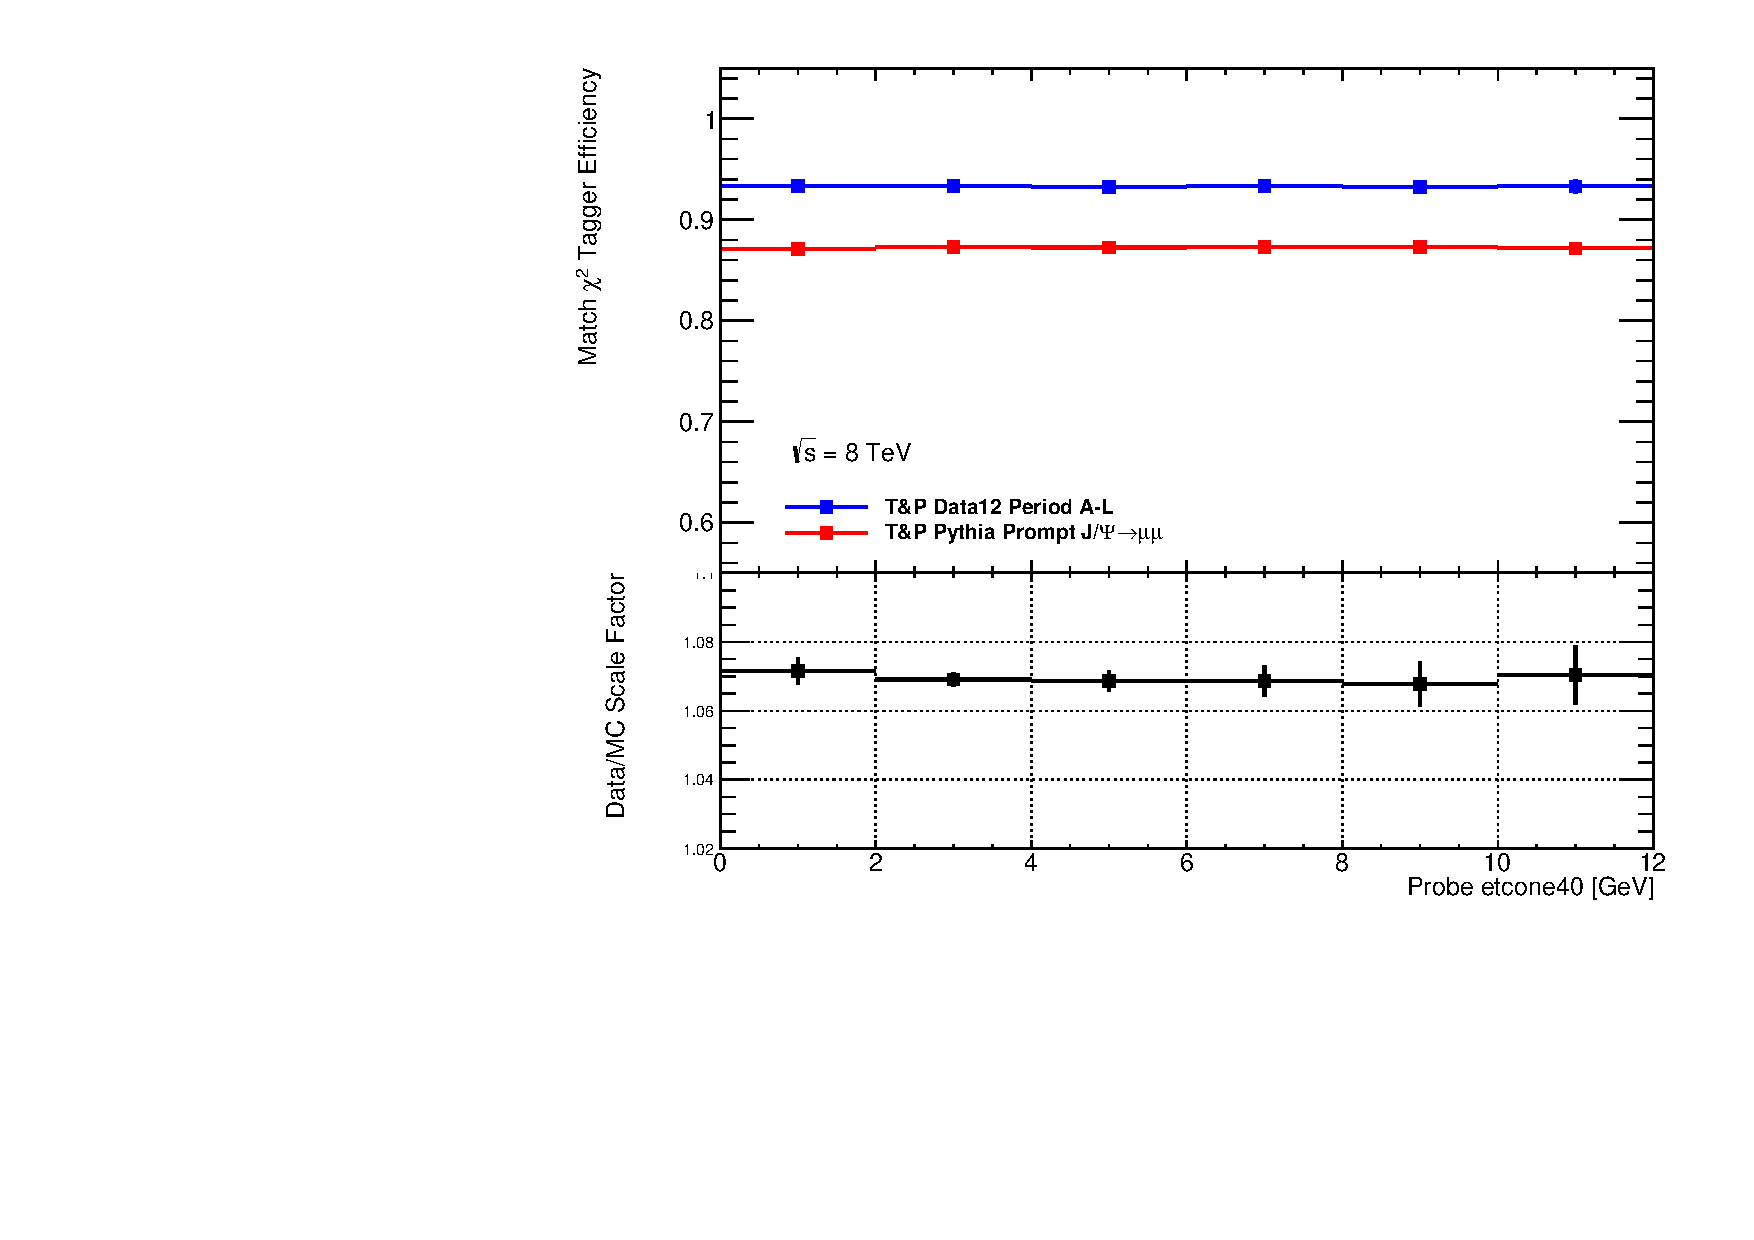
\includegraphics[width=\textwidth]{PartCalibration2012/Plots/SFPlots/etcone40_smt.pdf}
      \caption{$\sum \Et$ in cone $\Delta R=0.4$}\label{fig:CalibrationIsoEtcone40}
    \end{subfigure}
  \caption{\xsd\ efficiencies and scale factor with respect to $\sum \Et$ for a muon probe that passes the SMT requirements.}\label{fig:CalibrationIsoEtcone}
\end{figure}

% ptcone
\begin{figure}[htbp]
  \centering
    \begin{subfigure}[b]{0.76\textwidth}
      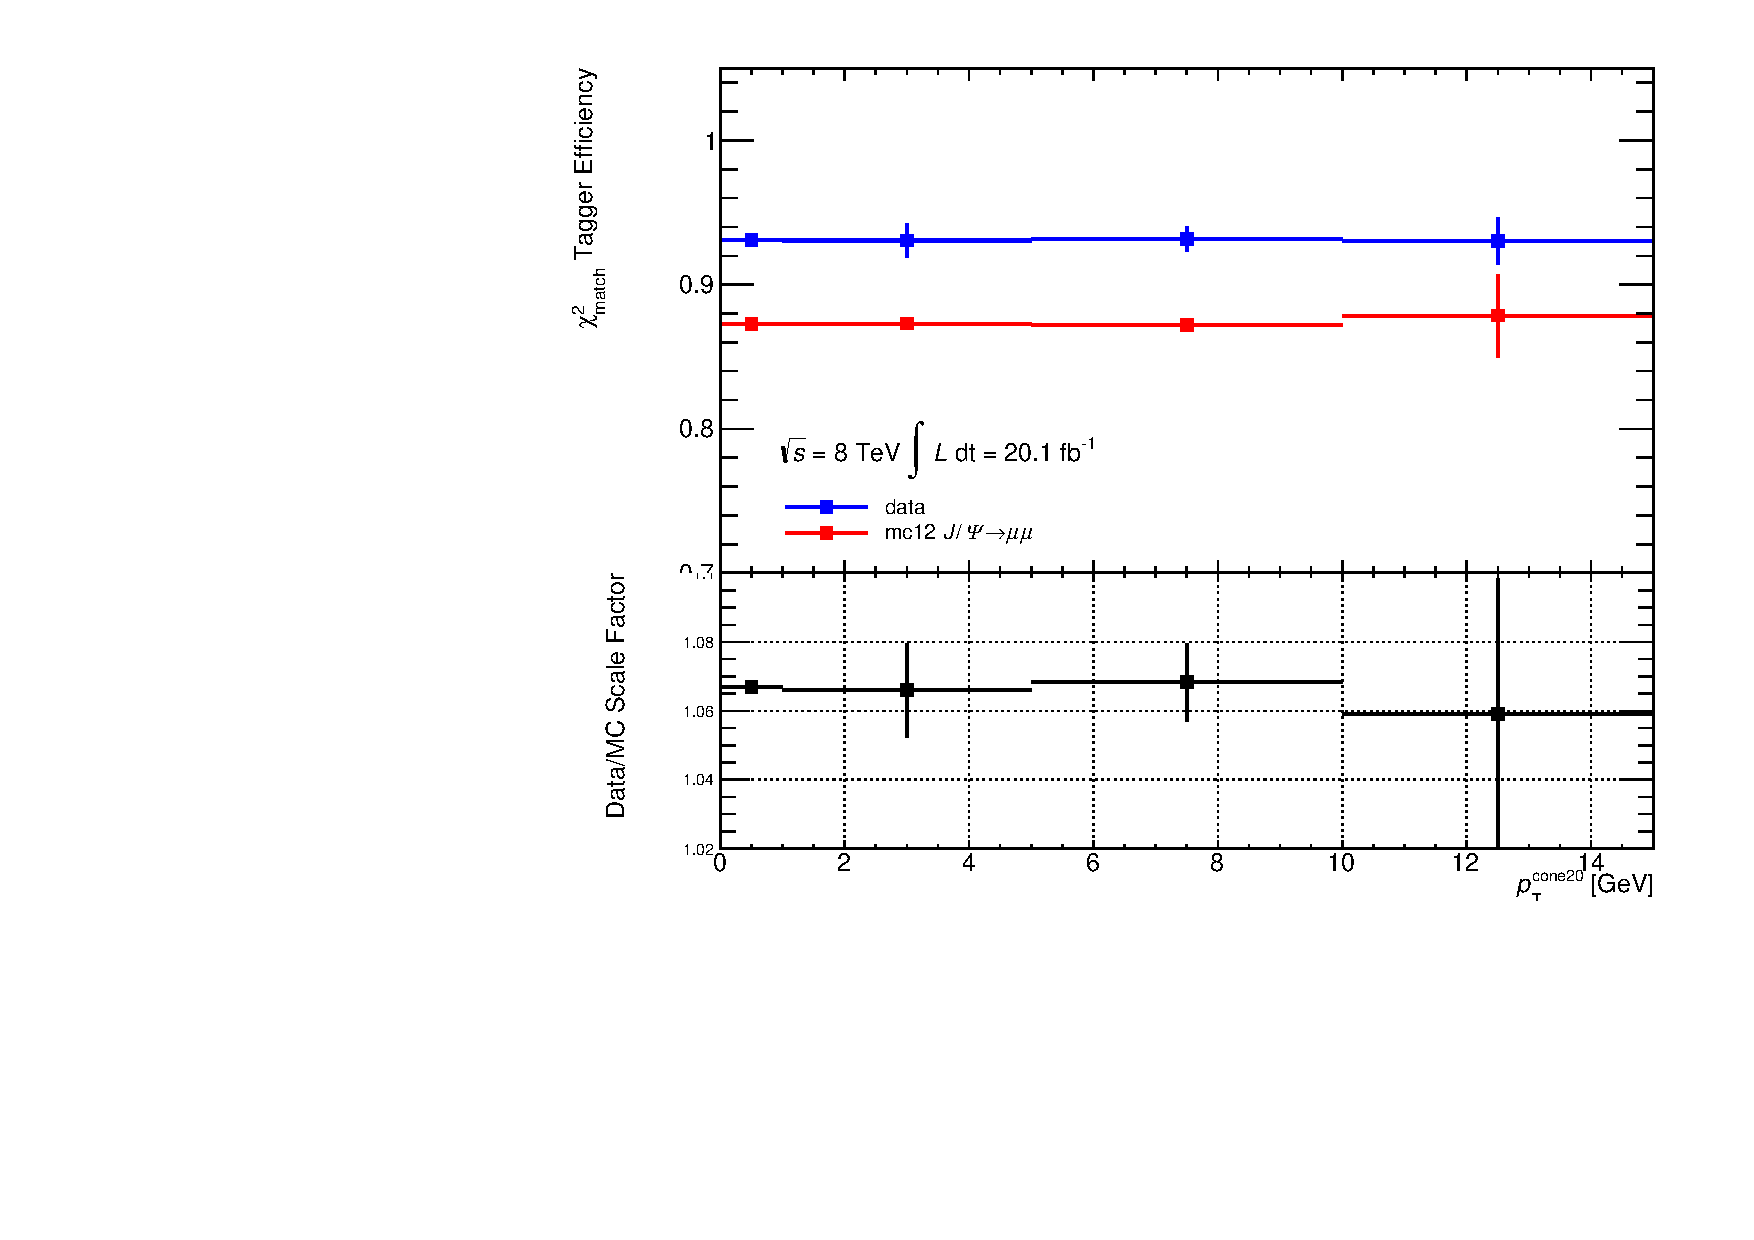
\includegraphics[width=\textwidth]{PartCalibration2012/Plots/SFPlots/ptcone20_smt.pdf}
      \caption{$\sum \pt$ in cone $\Delta R=0.2$}\label{fig:CalibrationIsoPtcone20}
    \end{subfigure}
    
    \begin{subfigure}[b]{0.76\textwidth}
      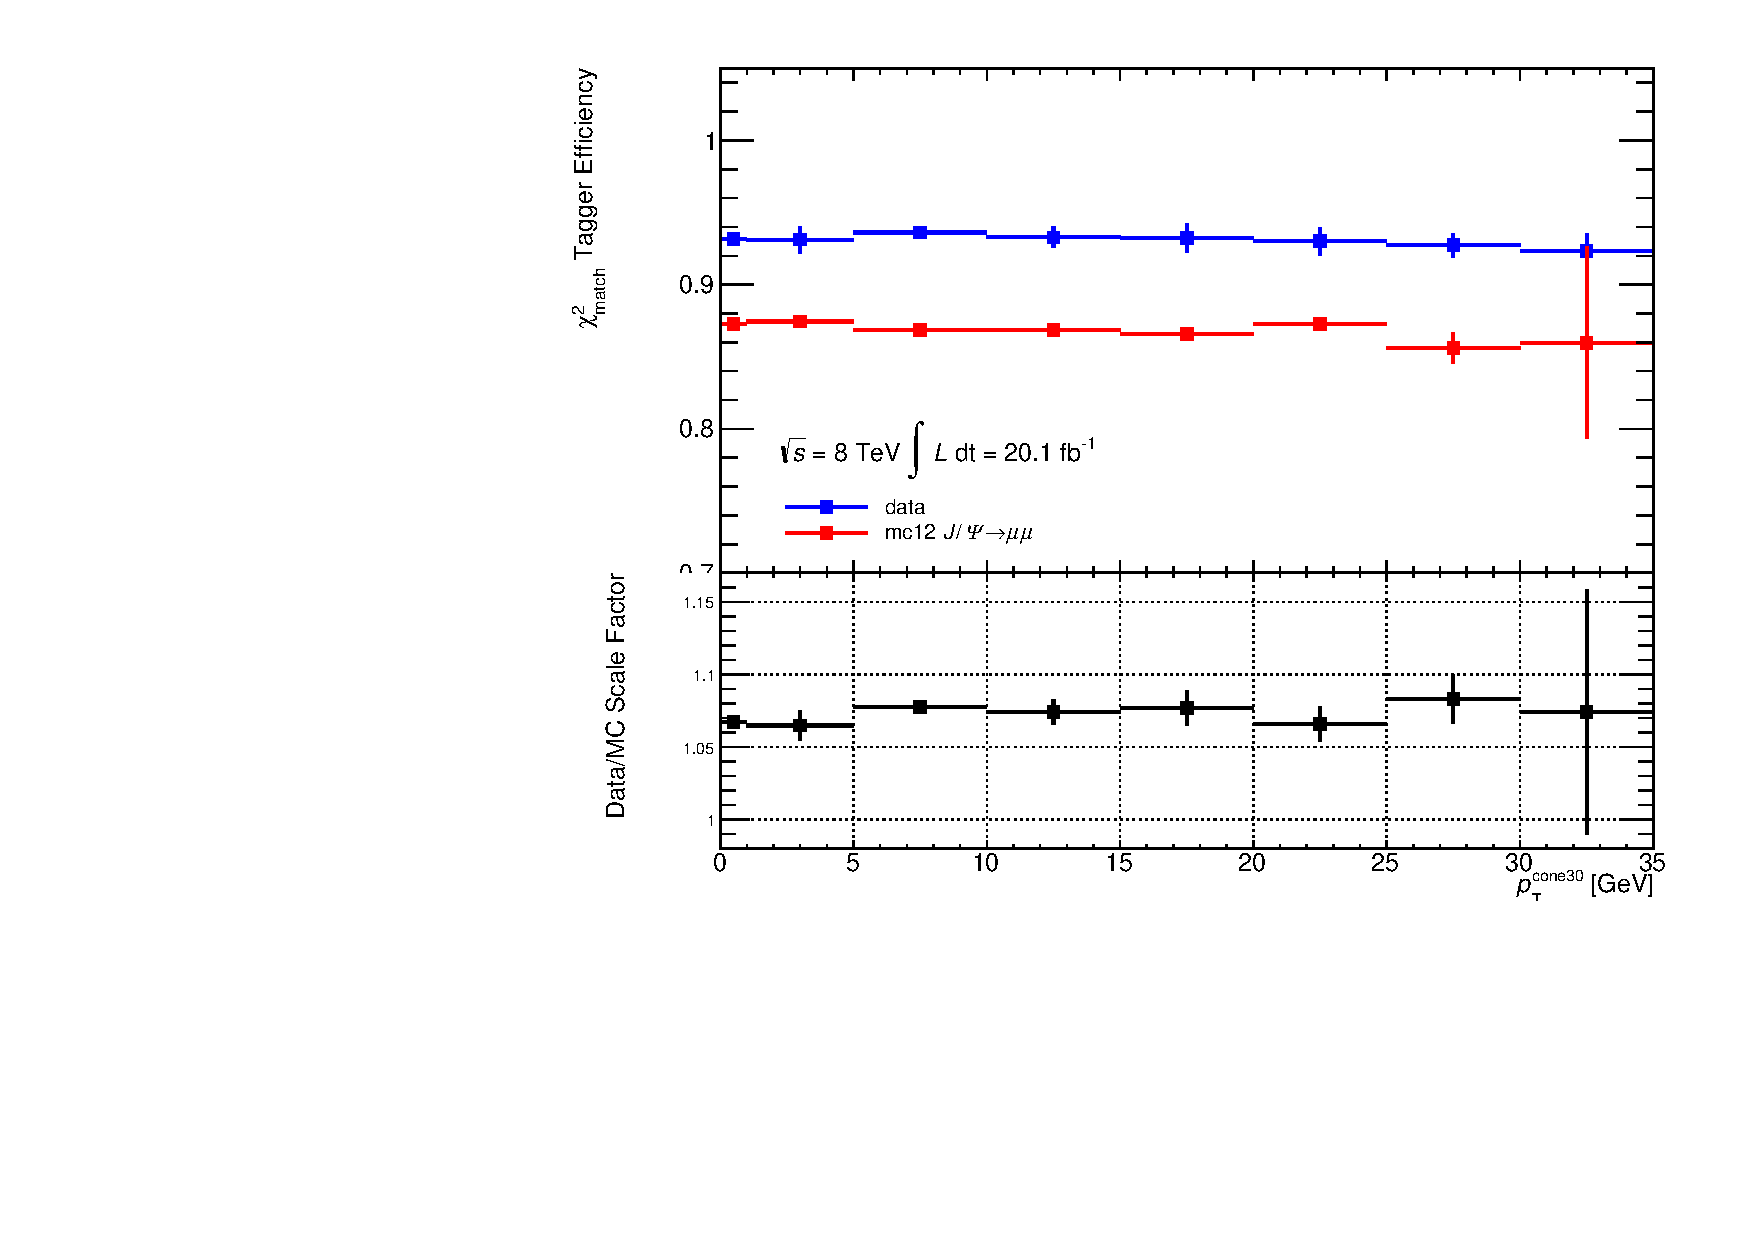
\includegraphics[width=\textwidth]{PartCalibration2012/Plots/SFPlots/ptcone30_smt.pdf}
      \caption{$\sum \pt$ in cone $\Delta R=0.3$}\label{fig:CalibrationIsoPtcone30}
    \end{subfigure}
    
    \begin{subfigure}[b]{0.76\textwidth}
      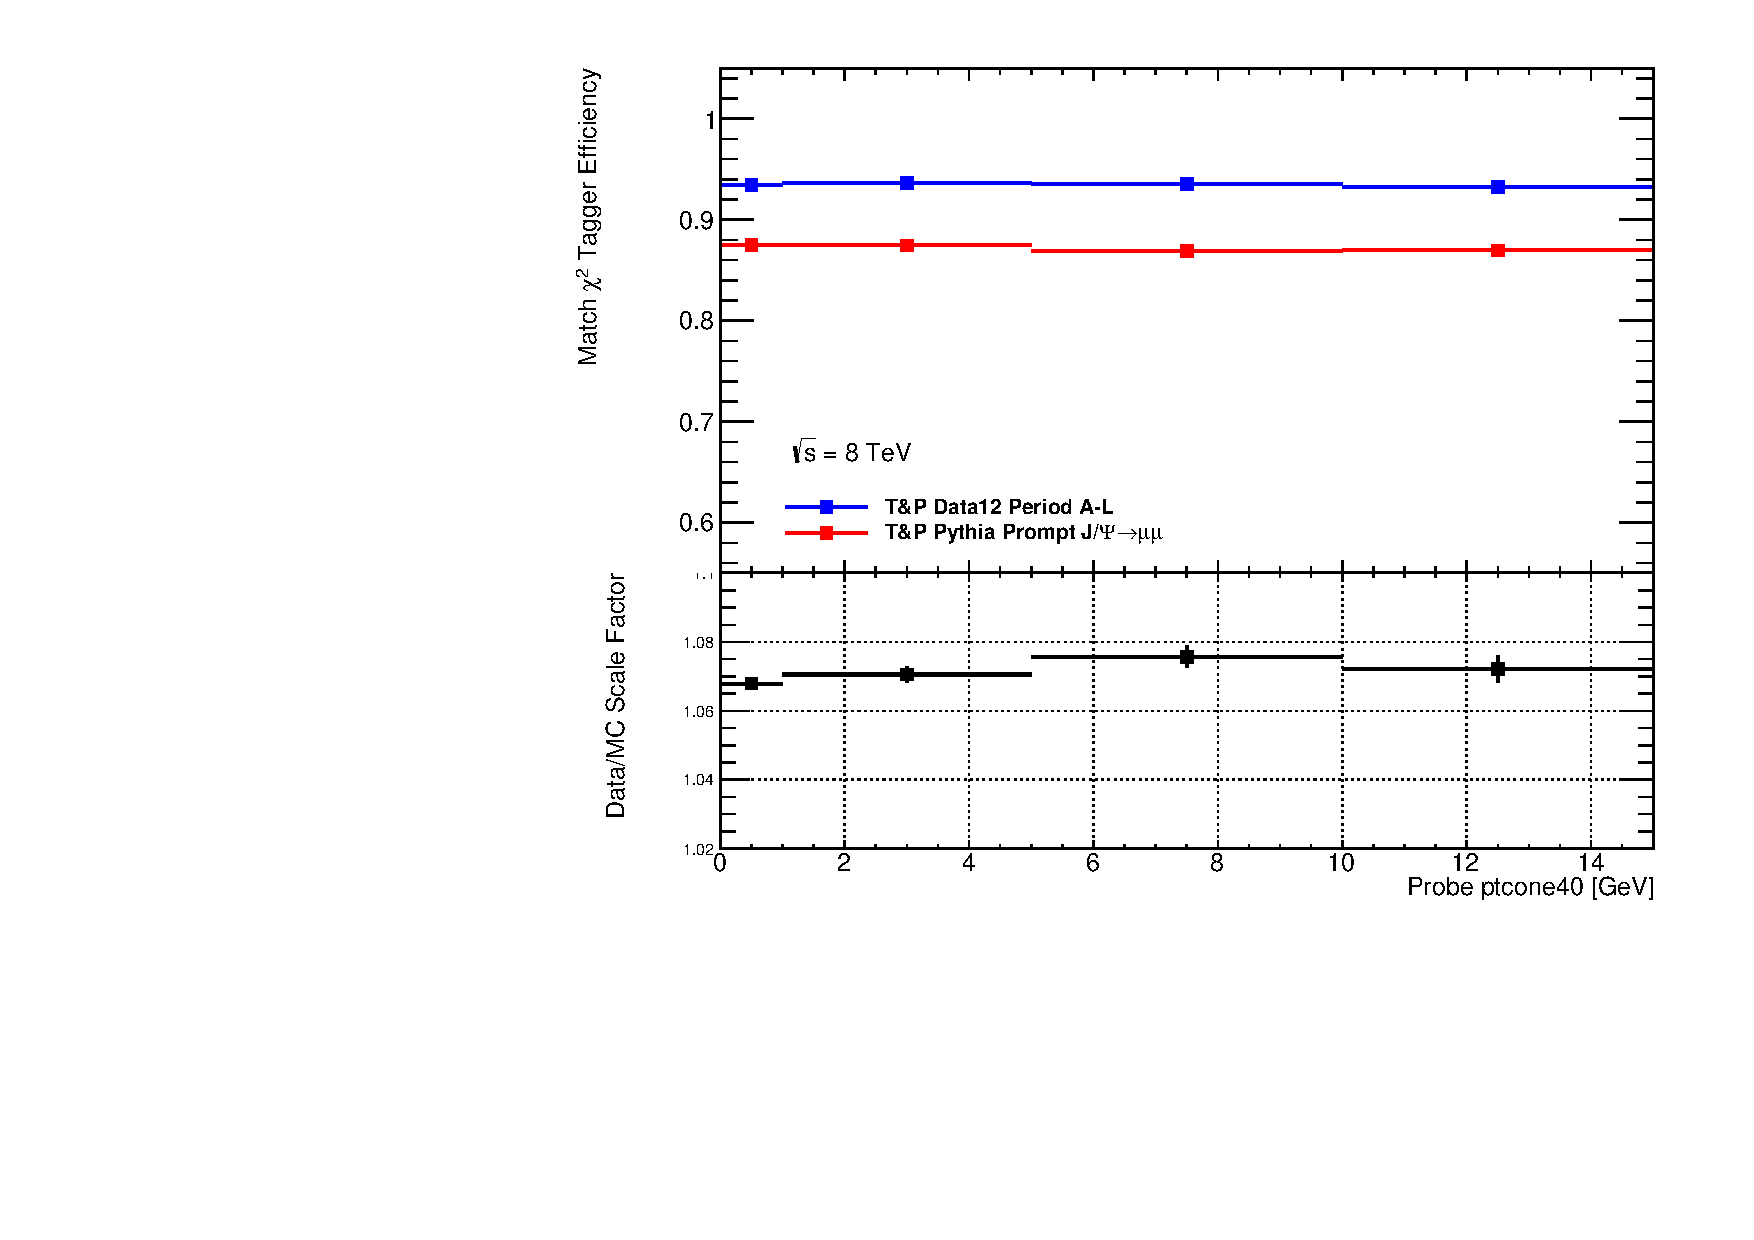
\includegraphics[width=\textwidth]{PartCalibration2012/Plots/SFPlots/ptcone40_smt.pdf}
      \caption{$\sum \pt$ in cone $\Delta R=0.4$}\label{fig:CalibrationIsoPtcone40}
    \end{subfigure}
  \caption{\xsd\ efficiencies and scale factor with respect to $\sum \pt$ for a muon probe that passes the SMT requirements.}\label{fig:CalibrationIsoPtcone}
\end{figure}

% nucone
\begin{figure}[htbp]
  \centering
    \begin{subfigure}[b]{0.76\textwidth}
      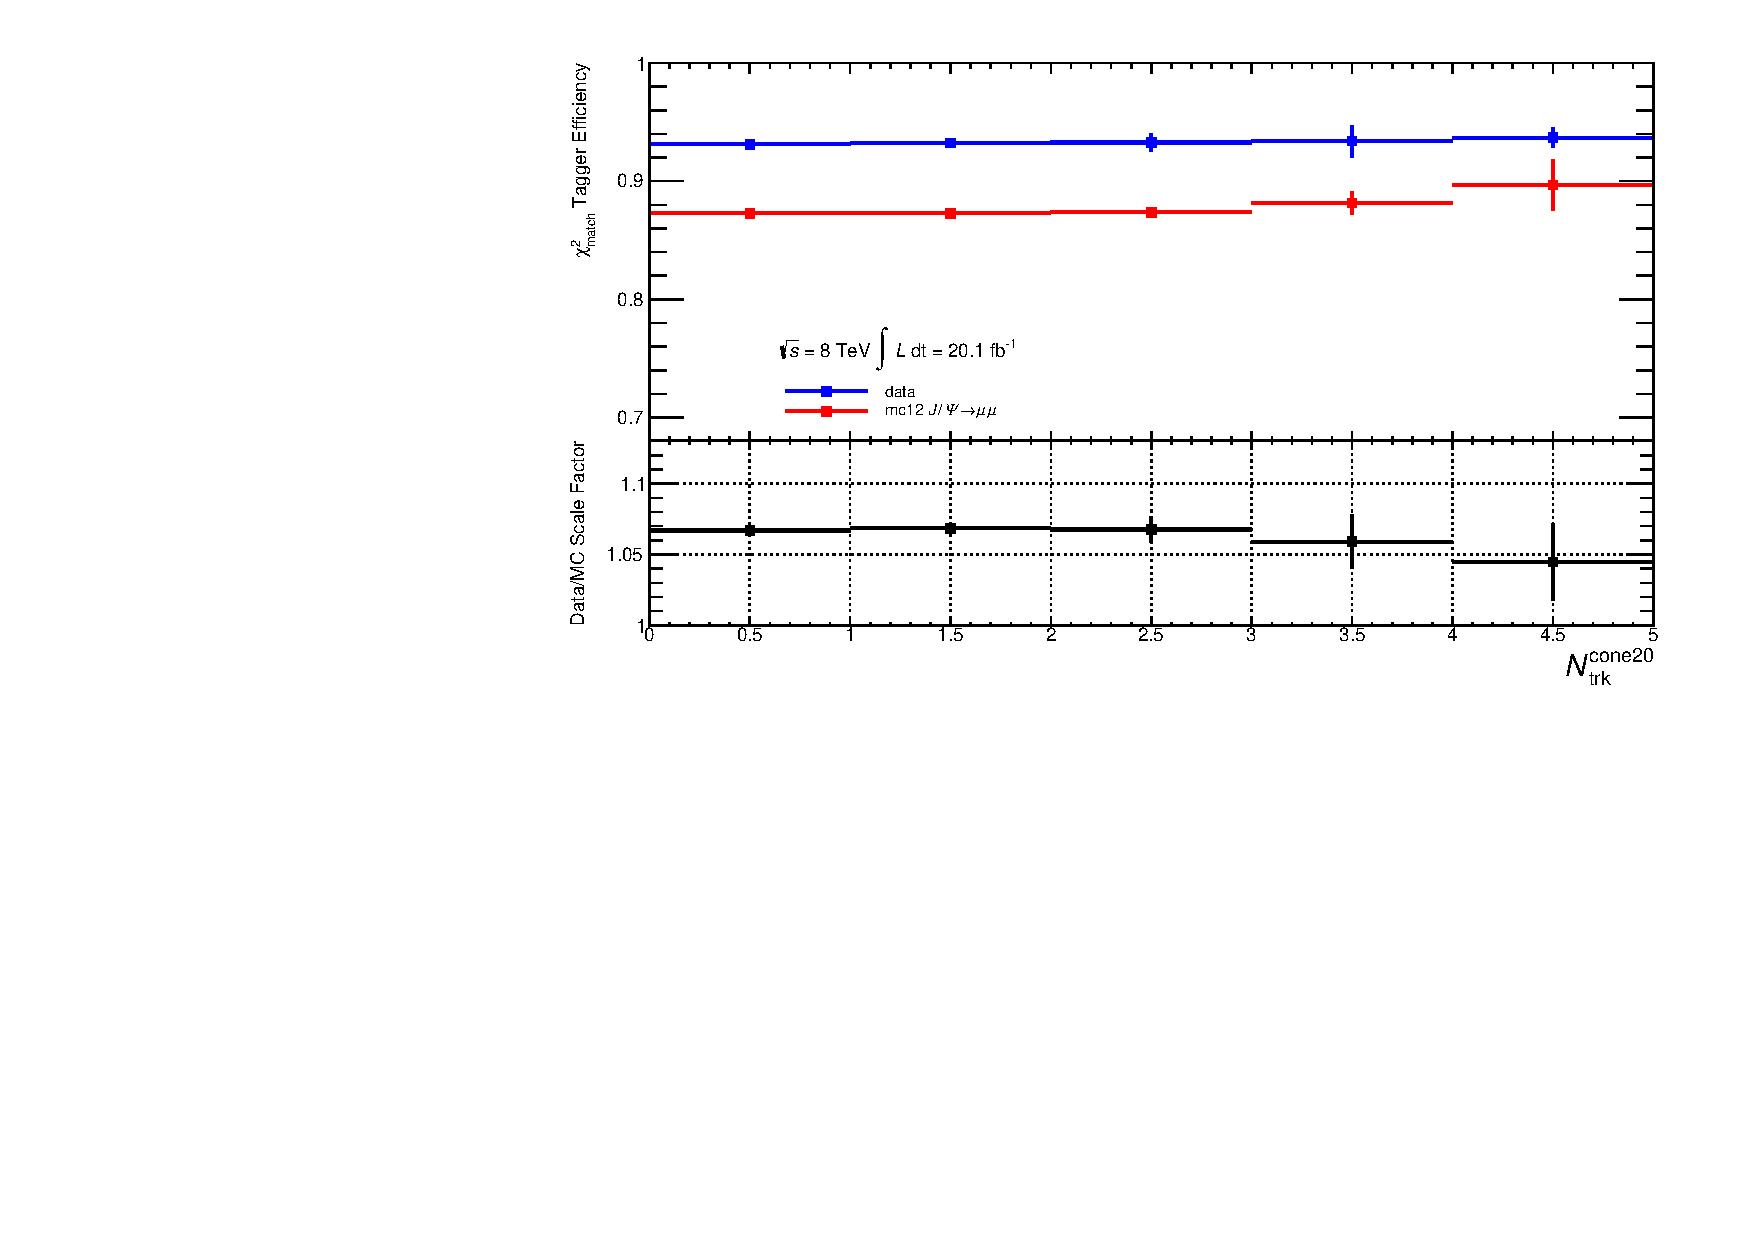
\includegraphics[width=\textwidth]{PartCalibration2012/Plots/SFPlots/nucone20_smt.pdf}  
      \caption{$N_{\textrm{trk}}$ in cone $\Delta R=0.2$}\label{fig:CalibrationIsoNucone20}
    \end{subfigure}
    
    \begin{subfigure}[b]{0.76\textwidth}
      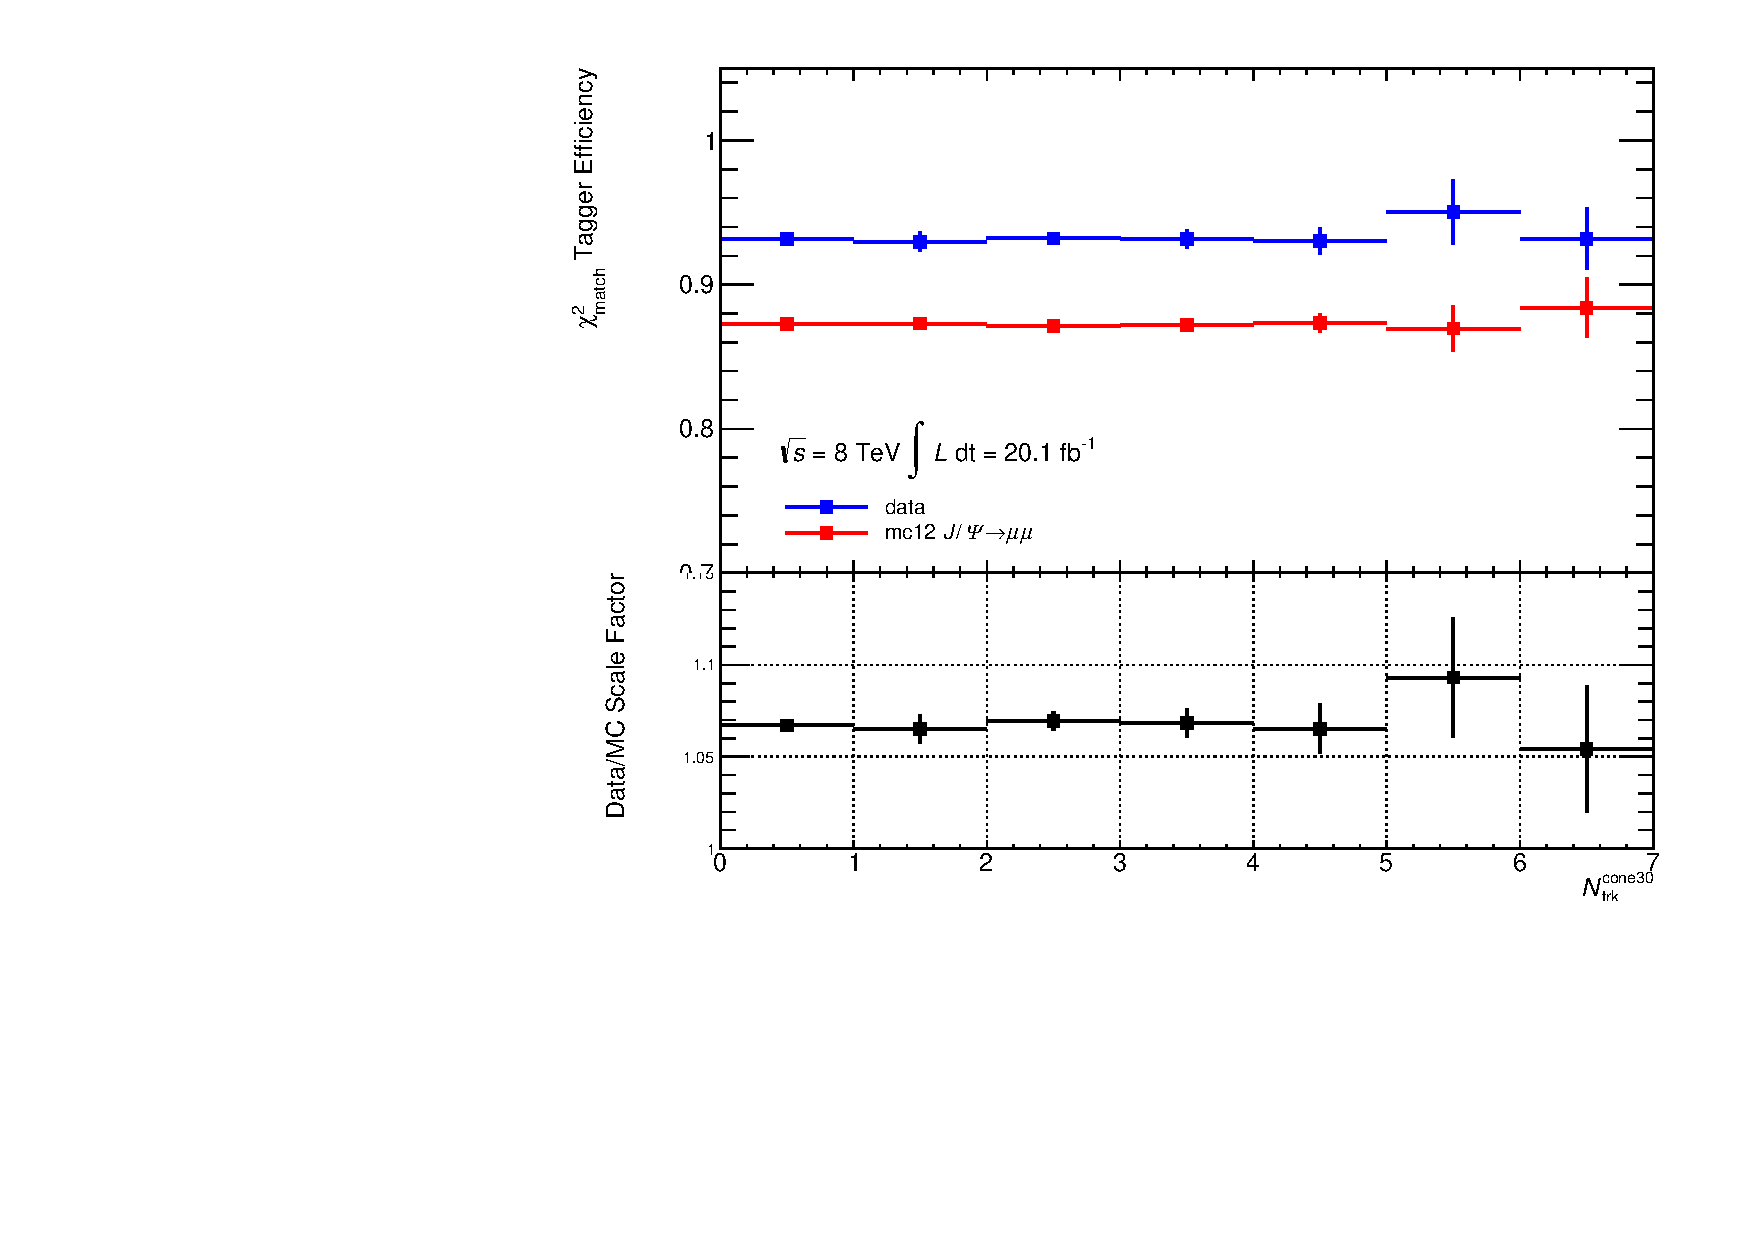
\includegraphics[width=\textwidth]{PartCalibration2012/Plots/SFPlots/nucone30_smt.pdf}
      \caption{$N_{\textrm{trk}}$ in cone $\Delta R=0.3$}\label{fig:CalibrationIsoNucone30}
    \end{subfigure}
    
    \begin{subfigure}[b]{0.76\textwidth}
      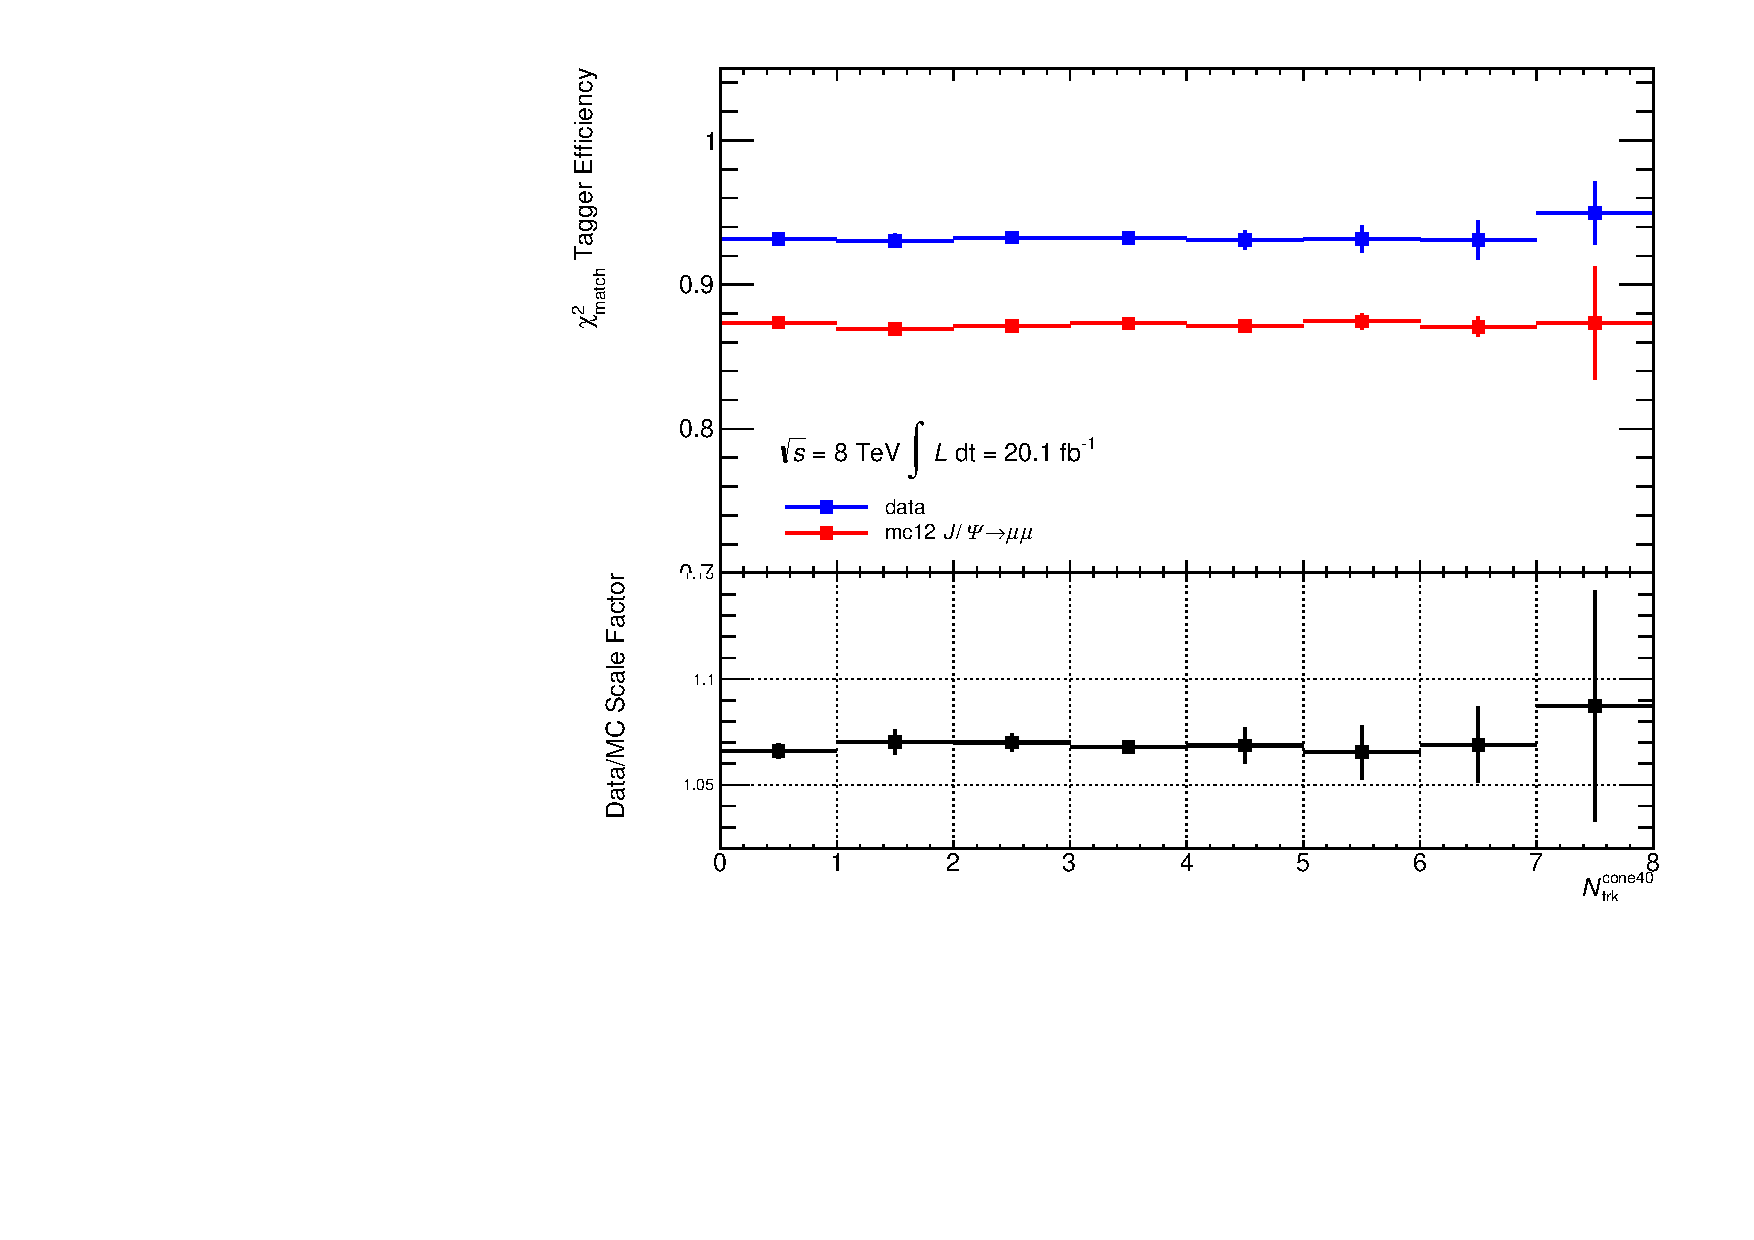
\includegraphics[width=\textwidth]{PartCalibration2012/Plots/SFPlots/nucone40_smt.pdf}
      \caption{$N_{\textrm{trk}}$ in cone $\Delta R=0.4$}\label{fig:CalibrationIsoNucone40}
    \end{subfigure}
  \caption{\xsd\ efficiencies and scale factor with to $N_{\textrm{tracks}}$ for a muon probe that passes the SMT requirements.}\label{fig:CalibrationIsoNucone}
\end{figure}

\subsubsection*{Dependence on $d_{0}$}

The dependence on the impact parameter $d_{0}$ was examined and no direct dependence is observed. The scale factor shows no structure with respect to $d_{0}$ when binned in \pt\ (Figure~\ref{fig:CalibrationD0Results}). Since the scale factors are binned in $\eta$ and \pt, the correlation between $d_{0}$ and \pt\ is taken into account.

\begin{figure}[htbp]
  \centering
  \sisetup{range-units=single}
  \begin{subfigure}[b]{0.74\textwidth}
    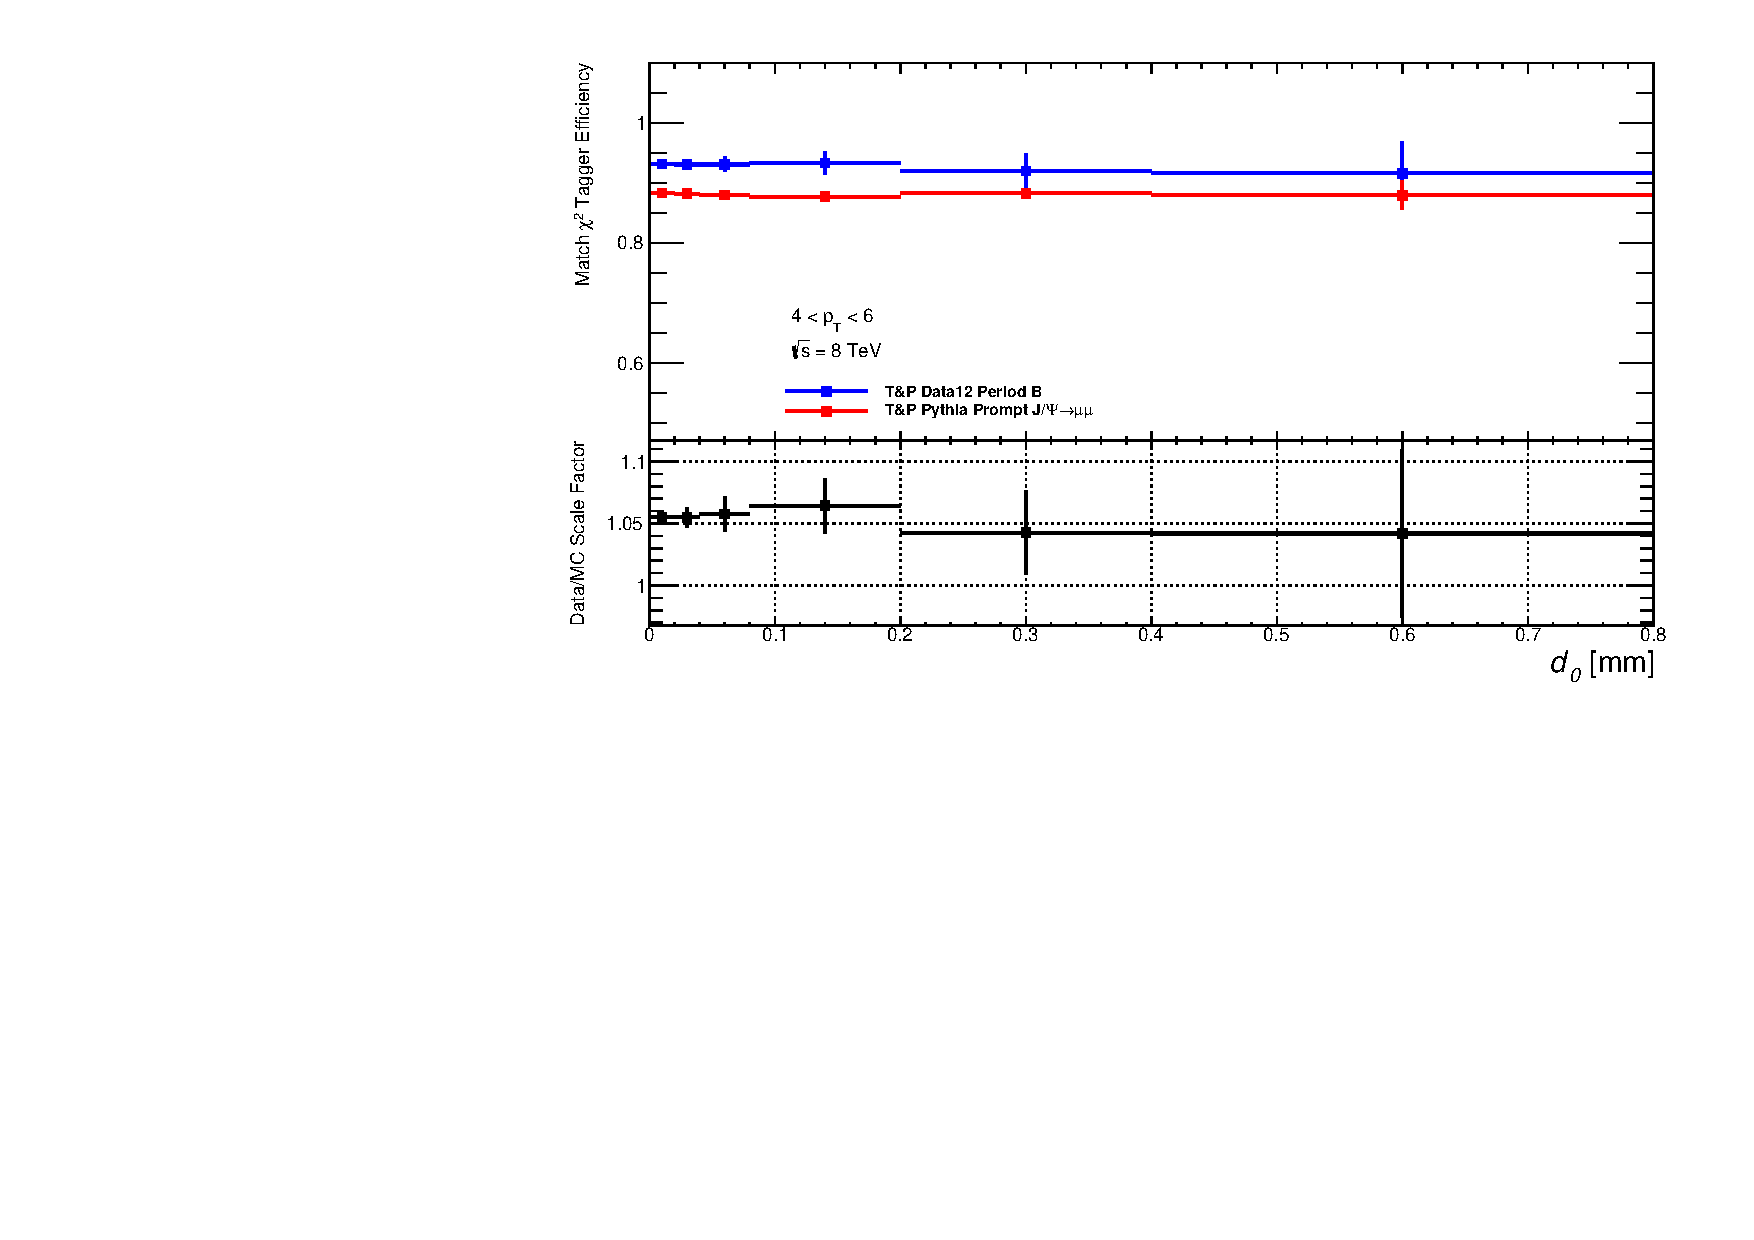
\includegraphics[width=\textwidth]{PartCalibration2012/Plots/SFPlots/ptCourse_4_6__smt.pdf}
    \caption{$\SI{4}{\GeV}<\pt<\SI{6}{\GeV}$}\label{fig:CalibrationD04to6}
  \end{subfigure}
  
  \begin{subfigure}[b]{0.74\textwidth}
    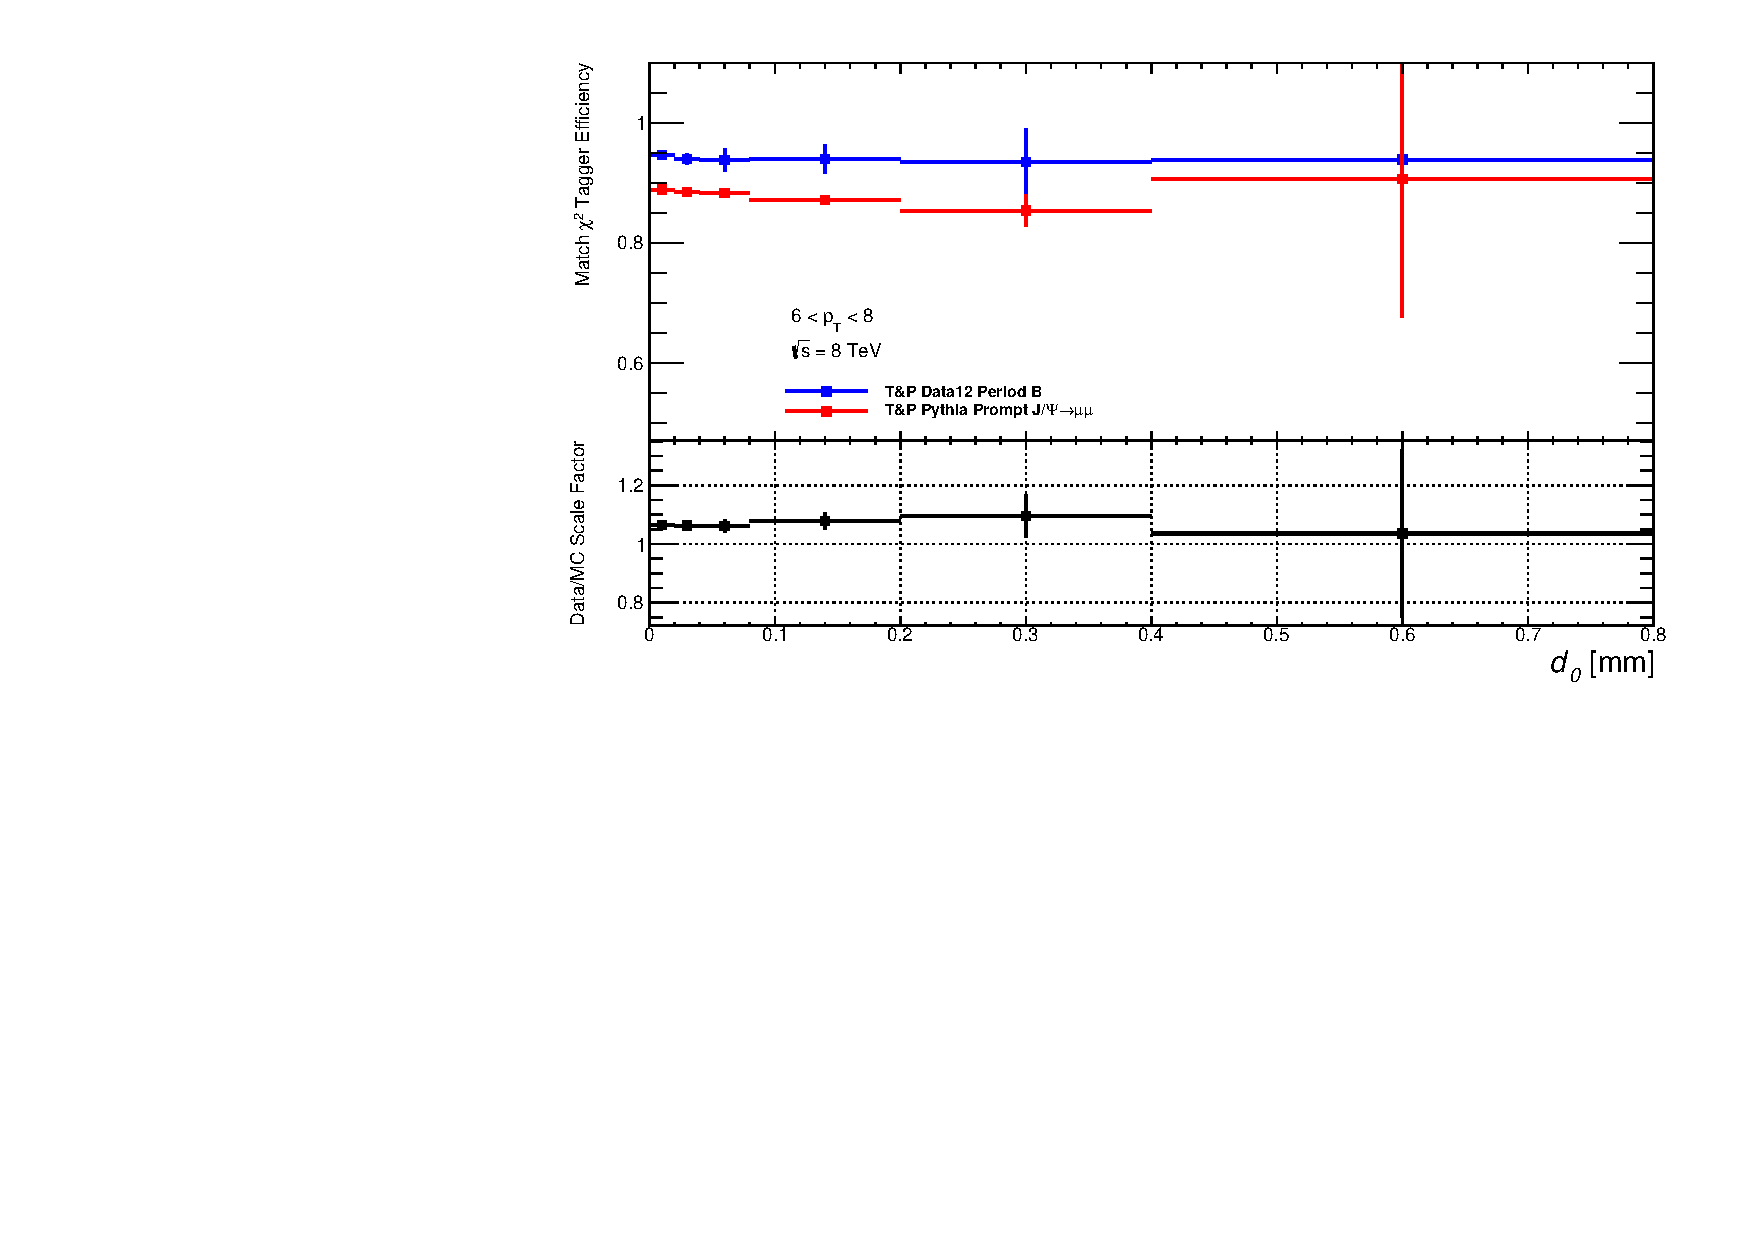
\includegraphics[width=\textwidth]{PartCalibration2012/Plots/SFPlots/ptCourse_6_8__smt.pdf}
    \caption{$\SI{6}{\GeV}<\pt<\SI{8}{\GeV}$}\label{fig:CalibrationD06to8}
  \end{subfigure}

  \begin{subfigure}[b]{0.74\textwidth}
    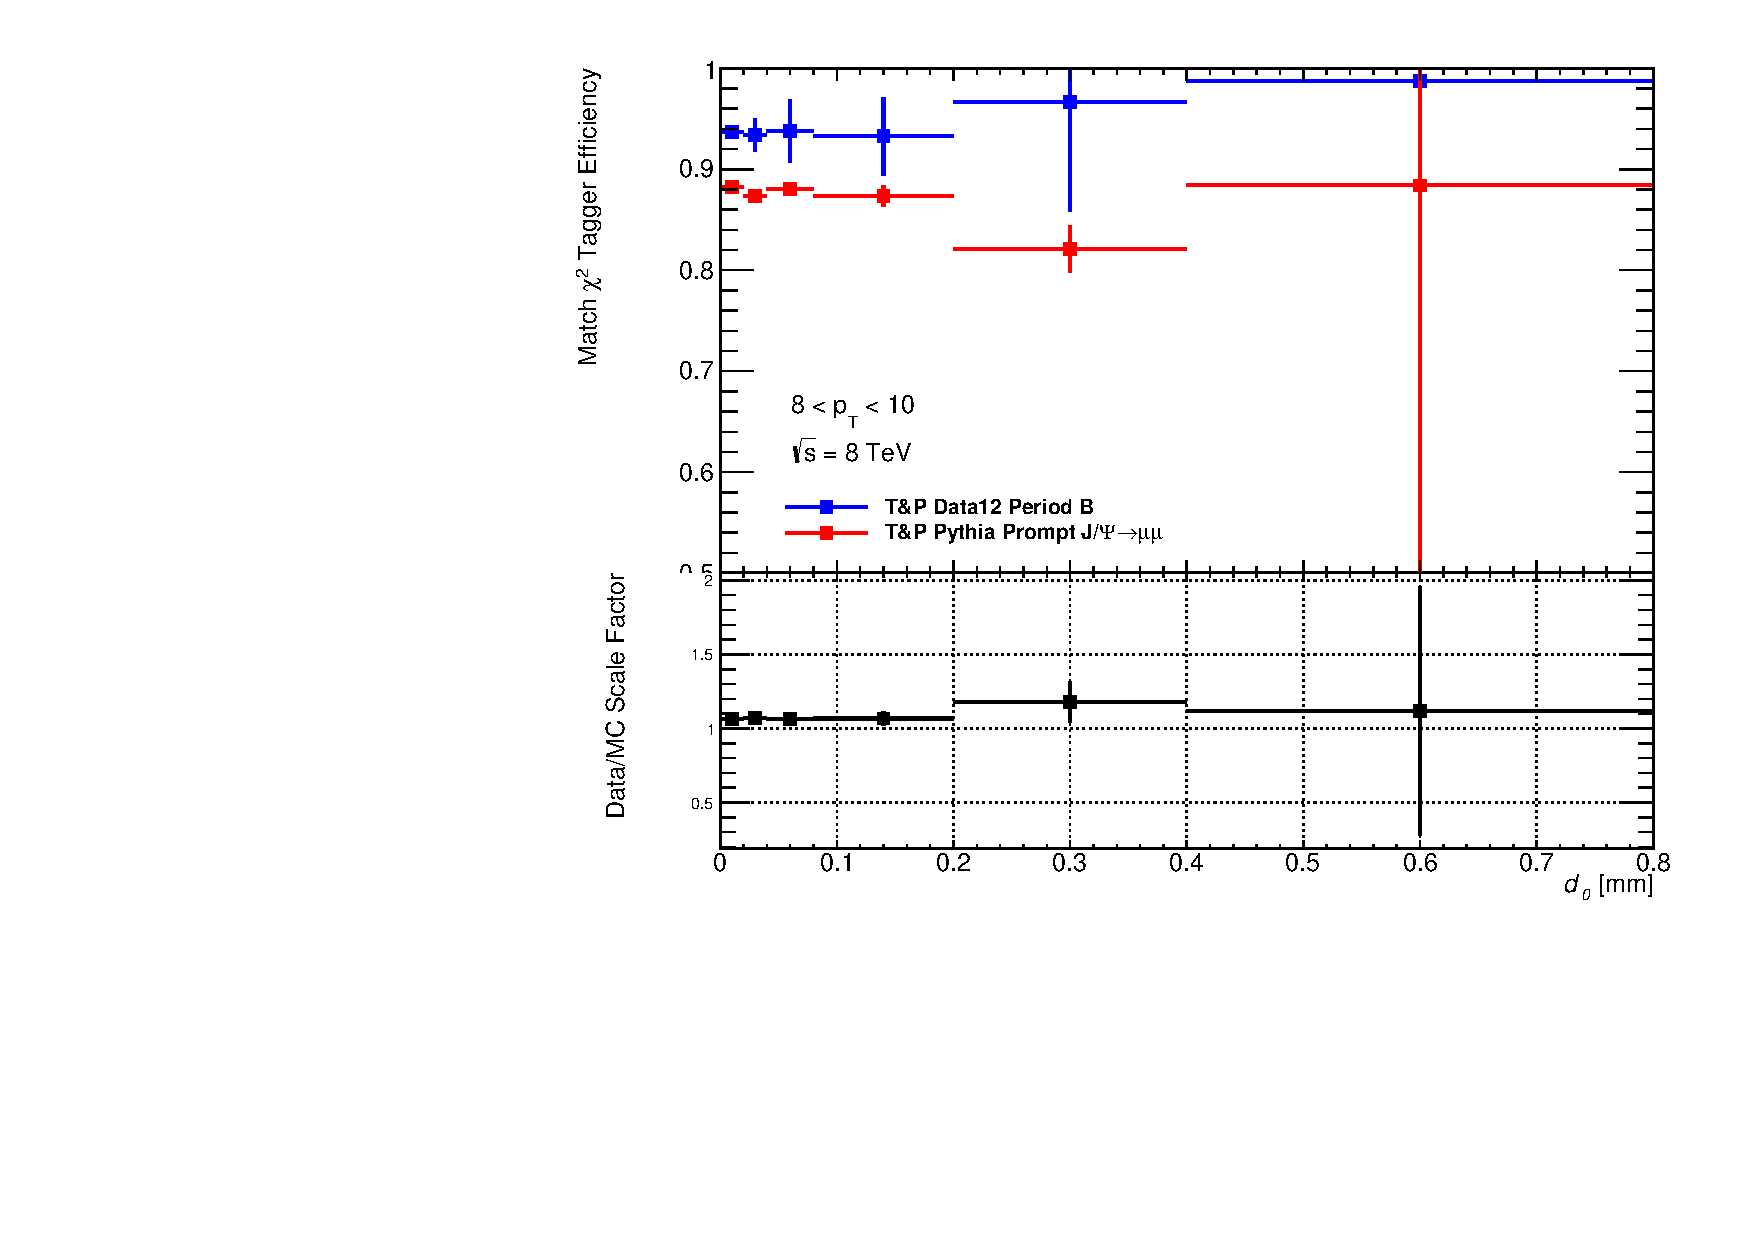
\includegraphics[width=\textwidth]{PartCalibration2012/Plots/SFPlots/ptCourse_8_10__smt.pdf}
    \caption{$\SI{8}{\GeV}<\pt<\SI{10}{\GeV}$}\label{fig:CalibrationD08to10}
  \end{subfigure}
  \caption[Distribution of the \xsm\ efficiencies and scale factor with respect to impact parameter $d_{0}$ for muon probes with \pt\ in the ranges \SIrange{4}{6}{\GeV}, \SIrange{6}{8}{\GeV} and \SIrange{8}{10}{\GeV}.]{Distribution of the \xsm\ efficiencies and scale factor with respect to impact parameter $d_{0}$ for muon probes with \pt\ in the ranges \subref{fig:CalibrationD04to6} \SIrange{4}{6}{\GeV}, \subref{fig:CalibrationD06to8} \SIrange{6}{8}{\GeV} and \subref{fig:CalibrationD08to10} \SIrange{8}{10}{\GeV}. The measurement was carried out only on Period B of 2012 ATLAS collision data.}\label{fig:CalibrationD0Results}
\end{figure}

\section{Scale factor discrepancy}

A discrepancy between the 2011 and 2012 scale factors is observed. The SFs in the 2011 analysis do not deviate substantially from unity, while the 2012 SFs deviate as much as \SI{15}{\percent}. The efficiency measured in the 2012 collision data appears to be consistent with the 2011 result, however in simulation the efficiency is measured to be lower. The difference in SF appears to come from a mismodelling of the \xsd\ variable. 

A number of factors can contribute to such a mismodelling including inaccurate description of the alignment of detector components, and the description of the material used in the detector. Both of these can result in mismodelling of the kinematic variables that make up the \xsd\ variable.

In order to find the source of the discrepancy the components of the \xsd\ variable were examined. The \emph{pull} of a kinematic variable is defined here as
%
\begin{equation}
  X_{\textrm{pull}} = \frac{X^{\textrm{ID}} - X^\textrm{MS}}{\sqrt{\sigma^{2}_{X^{\textrm{ID}}} + \sigma^{2}_{X^{\textrm{MS}}}}}
  \label{eq:CalibrationPull}
\end{equation}
%
where $X$ is any of the five kinematic components of \xsm, and $\sigma$ is the uncertainty on that variable. The pulls are shown in terms of the azimuthal angle, the polar angle, the longitudinal and transverse impact parameters and the charge over momentum ($q/p$) of the muon probe in in Figure~\ref{fig:CalibrationPull}. The transverse momentum is related to the $q/p$ by $\pt=|1/(q/p)|\sin(\theta)$ and the pseudorapidity is defined in terms of the angle $\theta$ in Section~\ref{ch:Detector}. All distributions appear to suffer from some mismodelling in MC, with the $\theta$ distributions being the worst. By construction the two variables are strongly correlated~\cite{Calibration:TrackingSlides}, so its not unexpected to observe a discrepancy simultaneously in both of these arguments. Such a discrepancy could be caused by a mismodelling of the alignment of the detector components.

% Pull Plots
\begin{figure}[htbp]
  \centering
    \begin{subfigure}[b]{0.49\textwidth}
      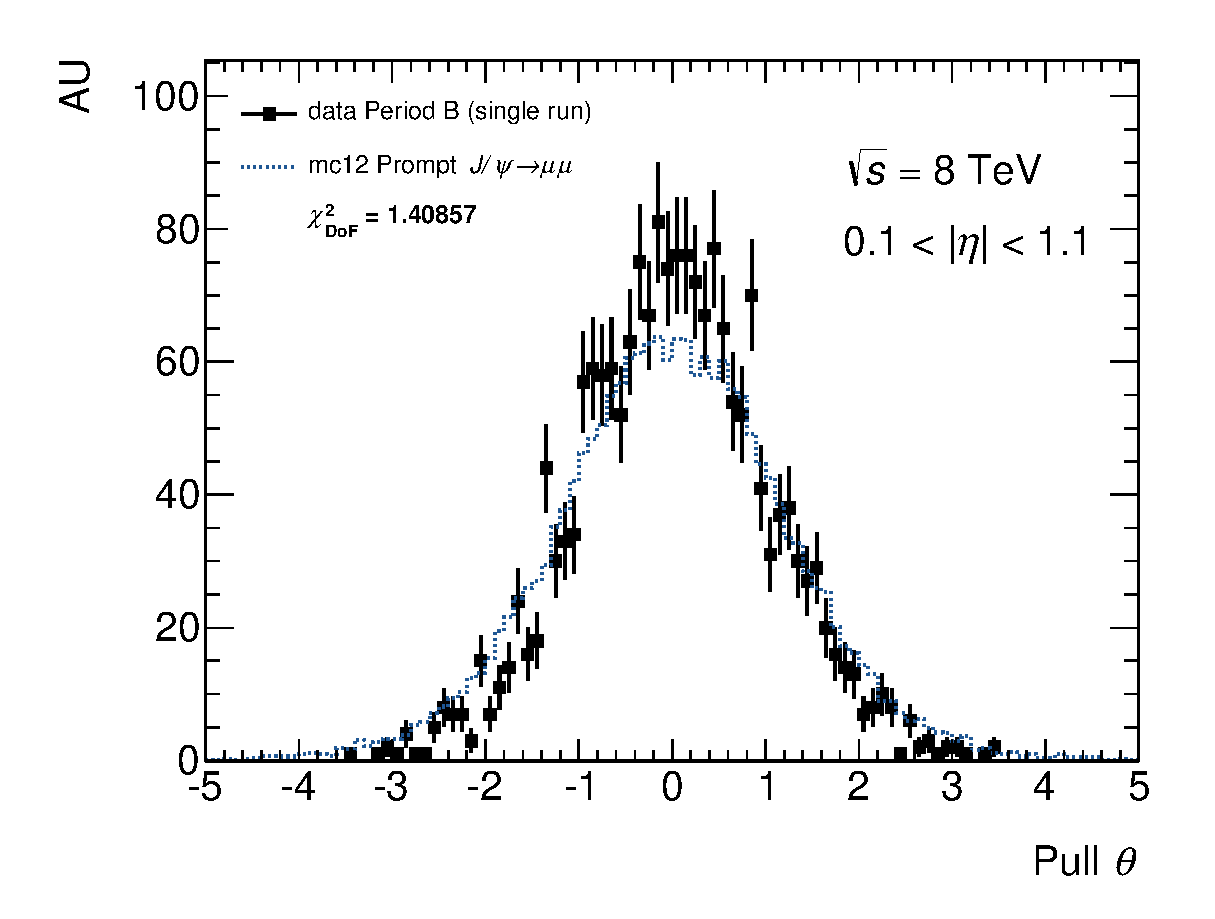
\includegraphics[width=\textwidth]{PartCalibration2012/Plots/DiscrepancyStudy/Pull/h_pull_theta_Nominal.eps}
      \caption{}\label{fig:CalibrationPullEta}
    \end{subfigure}
    \hfill
    \begin{subfigure}[b]{0.49\textwidth}
      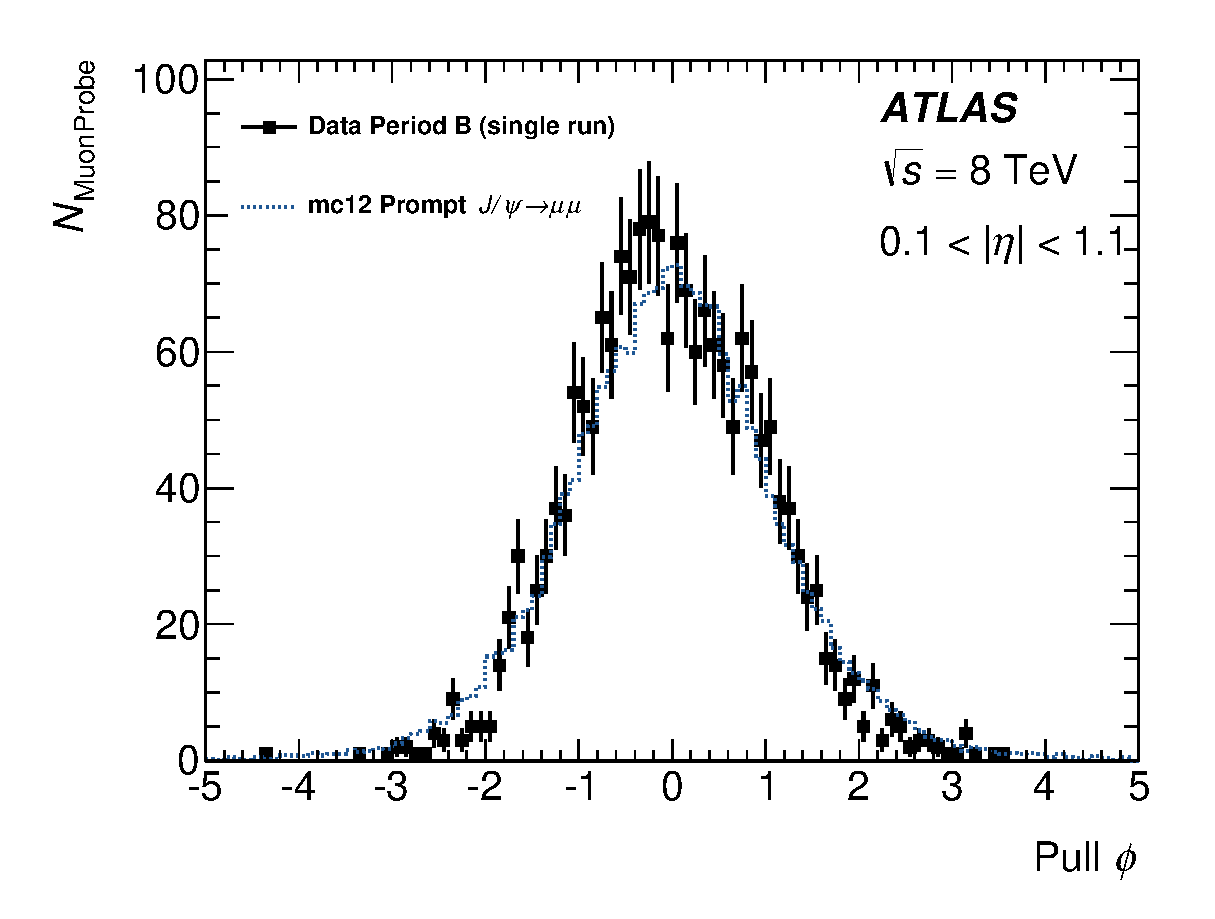
\includegraphics[width=\textwidth]{PartCalibration2012/Plots/DiscrepancyStudy/Pull/h_pull_phi_Nominal.eps}
      \caption{}\label{fig:CalibrationPullPhi}
    \end{subfigure}

    \begin{subfigure}[b]{0.49\textwidth}
      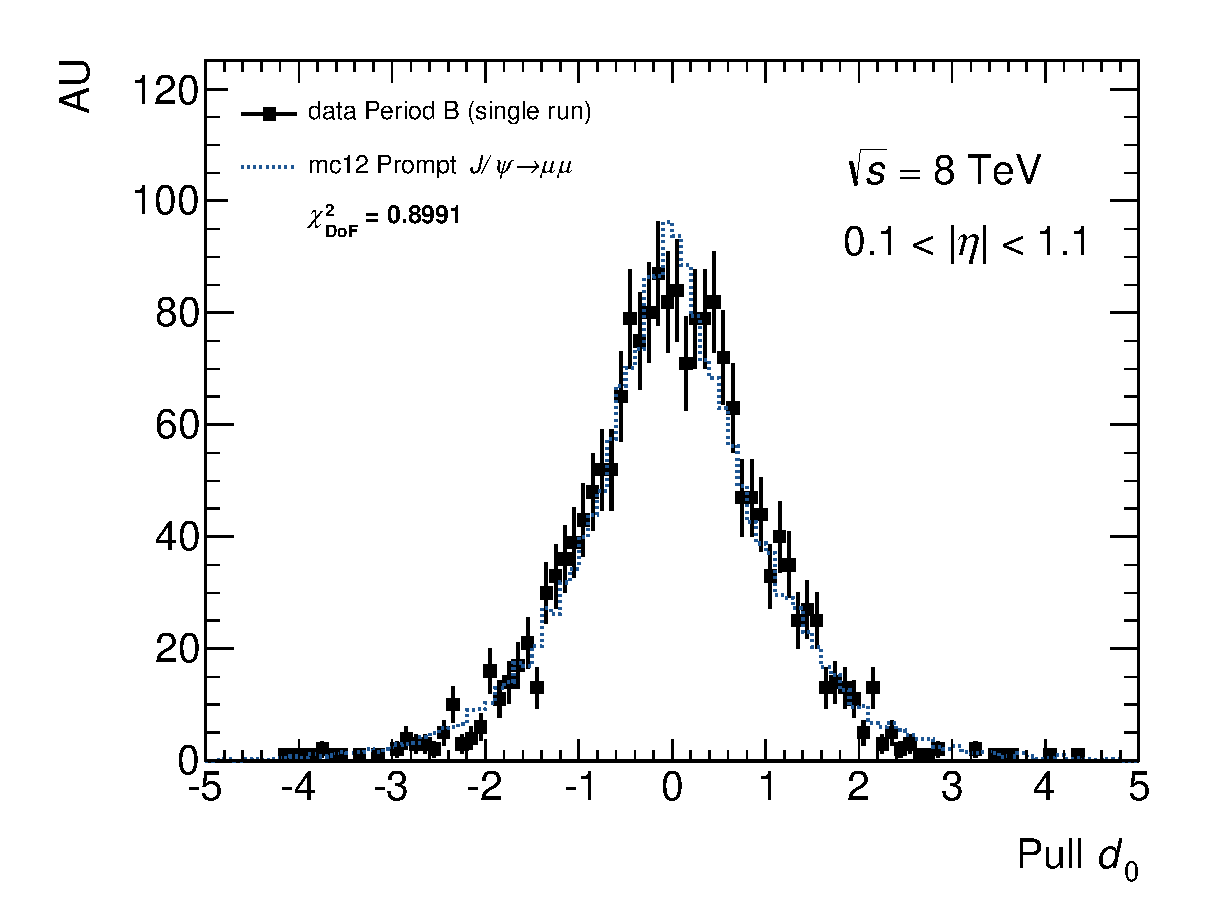
\includegraphics[width=\textwidth]{PartCalibration2012/Plots/DiscrepancyStudy/Pull/h_pull_d0_Nominal.eps}
      \caption{}\label{fig:CalibrationPullD0}
    \end{subfigure}
    \hfill
    \begin{subfigure}[b]{0.49\textwidth}
      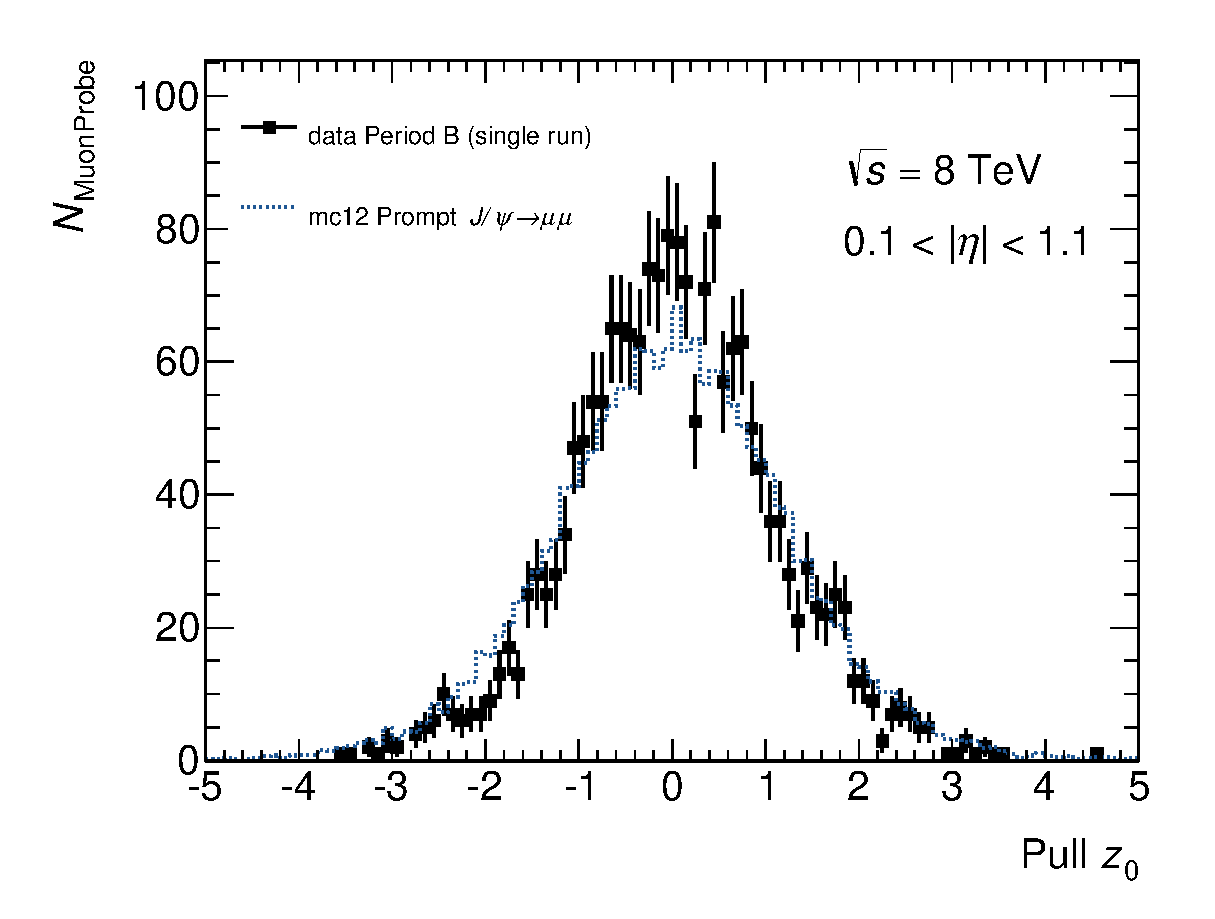
\includegraphics[width=\textwidth]{PartCalibration2012/Plots/DiscrepancyStudy/Pull/h_pull_z0_Nominal.eps}
      \caption{}\label{fig:CalibrationPullZ0}
    \end{subfigure}

    \begin{subfigure}[b]{0.49\textwidth}
      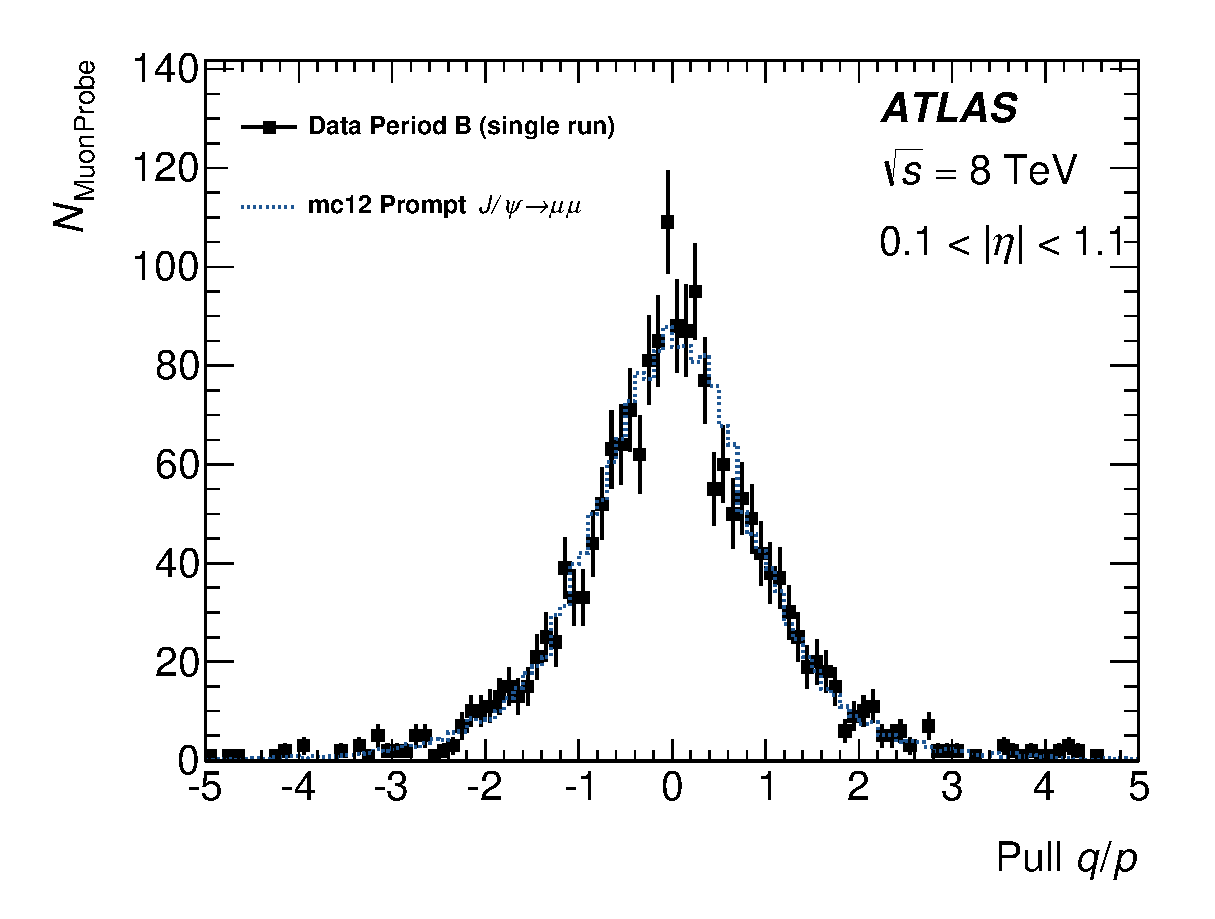
\includegraphics[width=\textwidth]{PartCalibration2012/Plots/DiscrepancyStudy/Pull/h_pull_qoverp_Nominal.eps}
      \caption{}\label{fig:CalibrationPullPt}
    \end{subfigure}
    \caption[Distribution of the pull of components of \xsd\ as measured in the ID for muon probes in the barrel region for collision data (squares) and prompt \jpsi\ simulation (dotted).]{Distribution of the pull (see~\ref{eq:CalibrationPull}) of components of \xsd\ as measured in the ID for muon probes in the barrel region for collision data (squares) and prompt \jpsi\ simulation (dotted). Shown are~\subref{fig:CalibrationPullEta} $\theta$,~\subref{fig:CalibrationPullPhi} $\phi$,~\subref{fig:CalibrationPullD0} $d_{0}$,~\subref{fig:CalibrationPullZ0} $z_{0}$ and~\subref{fig:CalibrationPullPt} $q$/$p$. Also shown is the goodness-of-fit \xsd\ between the collision data and the simulation. These distributions are based on smaller samples and are normalized to unit area.}\label{fig:CalibrationPull}
\end{figure}

A study to test the effects of different alignment profiles was carried out. Several samples with different alignment profiles were compared to a small sample of \SI{8}{\TeV} collision data from a single run. These include the nominal prompt \jpsi\ sample used in this calibration, the \jpsi\ sample used for the 2011 calibration, a \ZMu\ sample where the detector is perfectly aligned, a 2011 \ZMu\ sample with an updated detector geometry description, and a \ZMu\ sample with the nominal smeared alignment. The smeared alignment is produced by distorting the ideal alignment sample within the current measured alignment uncertainties. This procedure is not designed to perfectly represent the details in the misalignment of the ATLAS detector, but rather simulates a detector which is as well aligned as the real detector. These two profiles are compared in small samples of \ZMu\ events.

A sample of well reconstructed muons is selected by matching STACO CB muons to truth muons\footnote{These are the muons present in the truth information.} from $Z$ or \jpsi. The \xsd\ distribution of these muons is then compared for muons with \pt\ between \num{4} and \SI{25}{\GeV}.

As expected, the alignment profile does have an effect on the \xsd\ distribution, particularly in the lower end (Figure~\ref{fig:CalibrationAlignment}). However, this effect is not sufficiently large to account, on its own, for the discrepancy between simulation and data in all bins. A pseudo-efficiency of the \xsm\ selection is obtained by taking the area under the curve below \num{3.2} and dividing it to the total area. The results are summarized in Table~\ref{tab:CalibrationProfileEffs}. The overall difference between the 2011 and 2012 \jpsi\ samples is approximately \SI{5}{\percent}, not sufficient to cover the discrepancy between data and MC\@.

\begin{table}[htbp]
  \centering
  \begin{tabular}{@{}lS[table-format=2.2(1)]@{}}
    \toprule
    Sample                      & {Pseudo-efficiency [\si{\percent}]} \\
    \midrule
    \textbf{Data } $\boldsymbol{\cmsE}$ & 94.35(2) \\
    $\boldsymbol{\JMu}$ \\
    \tabin\ Nominal 2011         & 95.22(2) \\
    \tabin\ Nominal 2012         & 90.59(2) \\
    $\boldsymbol{\ZMu}$ \\
    \tabin\ Nominal 2012         & 92.44(3) \\
    \tabin\ Ideal alignment 2012 & 91.37(3) \\
    \tabin\ New geometry 2011    & 91.43(3) \\
    \bottomrule
  \end{tabular}
  \caption{Summary of \xsm\ tagger efficiencies as measured in all tested samples.}\label{tab:CalibrationProfileEffs}
\end{table}

\begin{figure}[htbp]
  \centering
    \includegraphics[width=0.85\textwidth]{PartCalibration2012/Plots/FixingMomImba/h\string_muon\string_matchchi2\string_ndof.eps}
    \caption{Distribution of \xsd\ of STACO CB muons from collision data (circle), a nominal 2012 \ZMu\ sample (solid), a 2012 \ZMu\ sample with ideal detector alignment (dashed), a 2011 \ZMu\ sample with updated detector description (dashed-double dot), \JMu\ with nominal alignment at \cmsE\ (solid) and \JMu\ with smeared alignment at \cmsS\ as used in the 2011 analysis (dotted). Distributions are normalized to unit area.}\label{fig:CalibrationAlignment}
\end{figure}

\subsection{Future developments}

As can be seen from Figure~\ref{fig:CalibrationPullPt}, the momentum appears to be well modelled in both data and simulation. As a result, an alternative variable known as the momentum imbalance is currently being studied. The momentum imbalance is defined as
%
\begin{equation}
  \textrm{Mom. Imb.} = \frac{p^{\textrm{ID}} - p^{\textrm{ME}}}{p^{\textrm{ID}}}
\end{equation}
%
where $p^{\textrm{ID}}$ is the momentum of the muon track as measured in the ID and $p^{\textrm{ME}}$ is measured in the MS extrapolated (ME) back to the primary vertex. This extrapolation takes into account the loss of momentum that occurs when the muon traverses through the detector material.

The momentum imbalance distribution for the aforementioned samples is shown in Figure~\ref{fig:CalibrationMomImba}. Measurements of the efficiency using momentum imbalance have been carried out, and the collision data results appear to be well-modelled in simulation. The selection using momentum imbalance requires $\textrm{Mom. Imb.}<\num{0.1}$ as background sources tend to peak above this threshold. From full studies currently being carried out, the momentum imbalance at this operating point exhibits similar performance to the \xsm\ version of the tagger.

The pseudo-efficiency for this selection as measured in the aforementioned samples are shown in Table~\ref{tab:CalibrationMomImbaProfileEffs}. These appear to be less affected by the transition from 2011 reconstruction and 2012 reconstruction techniques. In addition, changes in the detector alignment and geometry description affect the pseudo-efficiency substantially less than the \xsd\ selection. 

\begin{table}[htbp]
  \centering
    \begin{tabular}{@{}lS[table-format=2.2(1)]@{}}
      \toprule
      Sample                   & {Pseudo-efficiency [\si{\percent}]} \\
      \midrule
      $\boldsymbol{\JMu}$ \\
      \tabin\ Nominal 2011           & 92.81(2) \\
      \tabin\ Nominal 2012           & 93.57(2) \\
      $\boldsymbol{\ZMu}$ \\
      \tabin\ New geometry 2011      & 94.20(3) \\
      \tabin\ Nominal 2012           & 94.19(3) \\
      \tabin\ Ideal alignment 2012   & 94.46(2) \\
      \bottomrule
    \end{tabular}
    \caption{Summary of momentum imbalance efficiencies as measured in all tested samples.}\label{tab:CalibrationMomImbaProfileEffs}
\end{table}

\begin{figure}[htbp]
  \centering
    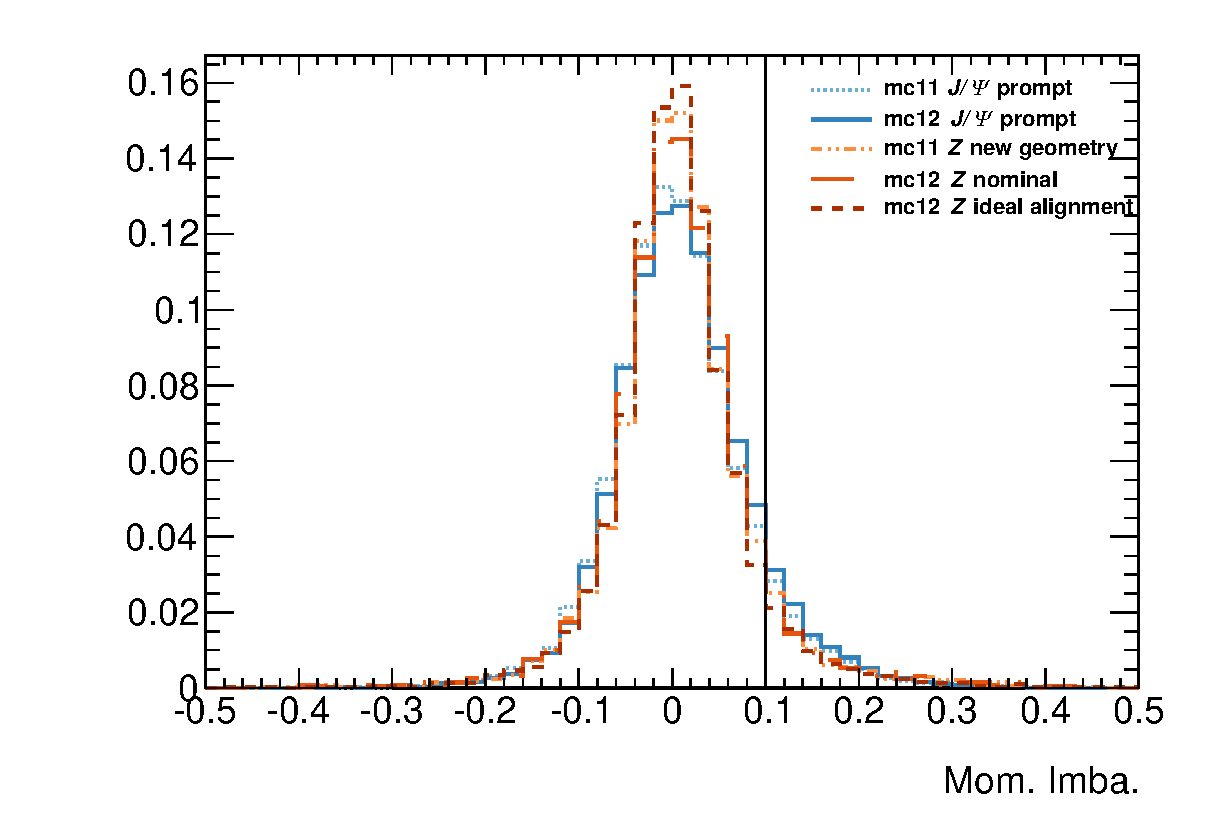
\includegraphics[width=0.85\textwidth]{PartCalibration2012/Plots/FixingMomImba/h_muon_momImba.eps}
    \caption{Distribution of momentum imbalance of STACO CB muons from a nominal 2012 \ZMu\ sample (solid), a 2012 \ZMu\ sample with ideal detector alignment (dashed), a 2011 \ZMu\ sample with updated detector description (dashed-double dot), \JMu\ with nominal alignment at \cmsE\ (solid) and \JMu\ with smeared at \cmsS\ as used in the 2011 analysis (dotted). Distributions are normalized to unit area.}\label{fig:CalibrationMomImba}
\end{figure}

Following a comparison of the reconstruction efficiencies with those obtained by members of the MCP group, the pairing selection has been loosened to allow for multiple probes per tag. It is possible for the correct probe to be further away from the tag in $z_0$ than other spurious tracks. By forcing the selection of the closest ID track in $z_0$, the sample of probes is contaminated with non-muons resulting in a lower than expected reconstruction efficiency. This increases the data available for invariant mass fitting and more importantly, has increased the reconstruction efficiency across the $\eta$-\pt\ phase space.

Overall, the mismodelling of \xsm\ in simulation cannot be fully explained in all tested bins by the description of the alignment alone. Additional testing could be performed on samples with different material description. If the \xsm\ distribution is substantially affected, this along with the alignment description could explain the difference between collision data and simulation.
